% Created 2023-08-12 Sat 22:48
% Intended LaTeX compiler: pdflatex
\documentclass[12pt,vi,leftblank,twoside]{mitthesis}
\usepackage[utf8]{inputenc}
\usepackage[T1]{fontenc}
\usepackage{graphicx}
\usepackage{longtable}
\usepackage{wrapfig}
\usepackage{rotating}
\usepackage[normalem]{ulem}
\usepackage{amsmath}
\usepackage{amssymb}
\usepackage{capt-of}
\usepackage{hyperref}
\usepackage{minted}
\usepackage{lgrind}
\usepackage{cmap}
\usepackage[T1]{fontenc}
\pagestyle{plain}
\usepackage[linesnumbered]{algorithm2e}
\usepackage{amsthm}
\usepackage{amsmath}
\usepackage{enumitem}
\usepackage{graphicx}
\usepackage{mathtools}
\usepackage{minted}
\usepackage[table,x11names]{xcolor}
\def\all{all}
\ifx\files\all \typeout{Including all files.} \else
\date{}
\title{Main SM Thesis Cover Abstract Acknowledgements Ch1 Introduction Problem Statement Approach Technical VDC Technical Scheduling Technical - Executive Technical Distributed Conclusion POSTNU to VDC Comparison Appendix - RMPL to STNUs}
\hypersetup{
 pdfauthor={Cameron W Pittman},
 pdftitle={Main SM Thesis Cover Abstract Acknowledgements Ch1 Introduction Problem Statement Approach Technical VDC Technical Scheduling Technical - Executive Technical Distributed Conclusion POSTNU to VDC Comparison Appendix - RMPL to STNUs},
 pdfkeywords={},
 pdfsubject={},
 pdfcreator={Emacs 28.2 (Org mode 9.6)}, 
 pdflang={English}}
\makeatletter
\newcommand{\citeprocitem}[2]{\hyper@linkstart{cite}{citeproc_bib_item_#1}#2\hyper@linkend}
\makeatother

\usepackage[notquote]{hanging}
\begin{document}

%% The documentclass options along with the pagestyle can be used to generate
%% a technical report, a draft copy, or a regular thesis. You may need to
%% re-specify the pagestyle after you \include cover.tex. For more
%% information, see the first few lines of mitthesis.cls.
%%
%\documentclass[12pt,vi,twoside]{mitthesis}
%%
%%  If you want your thesis copyright to you instead of MIT, use the
%%  ``vi'' option, as above.
%%
%\documentclass[12pt,twoside,leftblank]{mitthesis}
%%
%% If you want blank pages before new chapters to be labelled ``This
%% Page Intentionally Left Blank'', use the ``leftblank'' option, as
%% above.

%% These have been added at the request of the MIT Libraries, because
%% some PDF conversions mess up the ligatures.  -LB, 1/22/2014
%% This bit allows you to either specify only the files which you wish to
%% process, or `all' to process all files which you \include.
%% Krishna Sethuraman (1990).

%\typein [\files]{Enter file names to process, (chap1,chap2 ...), or `all' to process all files:}
%\typeout{Including only \files.} \includeonly{\files} \fi

\hypersetup{
  pdfauthor={Cameron W. Pittman},
  pdftitle={Distributed Multi-Agent Decision Making Under Uncertain Communication},
  pdfkeywords={},
  pdfsubject={},
  pdfcreator={Emacs 28.2 (Org mode 9.6)},
  pdflang={English}}

\usemintedstyle[lisp]{vs}

\graphicspath{{images/}}

\newcommand{\edge}[3]{#1 \xrightarrow{#3} #2}
\newcommand{\conedge}[3]{#1 \xRightarrow{#3} #2}
\newcommand{\gammabar}{\bar{\gamma}}
\newcommand{\fdelayedge}[4]{#1 \xRightarrow{#3} \stackrel{\gamma = #4}{#2}}
\newcommand{\vdelayedge}[4]{#1 \xRightarrow{#3} \stackrel{\bar{\gamma} \in #4}{#2}}
%\newcommand{\obs}{\texttt{obs}}
\newcommand{\obs}{\mathtt{obs}}
\newcommand{\assign}{\xi}

\newcommand{\finalversion}[1]{}

\newtheorem{theorem}{Theorem}[]
\newtheorem{corollary}{Corollary}[theorem]
\newtheorem{lemma}[theorem]{Lemma}

\newtheorem{transformation}{Transformation}

\theoremstyle{definition}
\newtheorem{defn}{Definition}

\theoremstyle{definition}
\newtheorem{example}{Example}

% org mode likes to add too much vertical spacing to lists
\setlist{noitemsep}

% NOTE:
% These templates make an effort to conform to the MIT Thesis specifications,
% however the specifications can change. We recommend that you verify the
% layout of your title page with your thesis advisor and/or the MIT
% Libraries before printing your final copy.

% FYI, the title and thesis need to be defined in the \hypersetup section in the main org file
\title{Distributed Multi-Agent Decision Making Under Uncertain Communication}
\author{Cameron W. Pittman}

% If you wish to list your previous degrees on the cover page, use the
% previous degrees command:
% You can use the \\ command to list multiple previous degrees
\prevdegrees{M.A., Belmont University (2011) \\
    B.A., Vanderbilt University (2009)}

\department{Department of Aeronautics and Astronautics}

% If the thesis is for two degrees simultaneously, list them both
% separated by \and like this:
% \degree{Doctor of Philosophy \and Master of Science}
\degree{Master of Science in Aeronautics and Astronautics}

% As of the 2007-08 academic year, valid degree months are September,
% February, or June.  The default is June.
\degreemonth{September}
\degreeyear{2023}
\thesisdate{August 15, 2023}

%% By default, the thesis will be copyrighted to MIT.  If you need to copyright
%% the thesis to yourself, just specify the `vi' documentclass option.  If for
%% some reason you want to exactly specify the copyright notice text, you can
%% use the \copyrightnoticetext command.
%\copyrightnoticetext{\copyright IBM, 1990.  Do not open till Xmas.}

% If there is more than one supervisor, use the \supervisor command
% once for each.
\supervisor{Brian C. Williams}{Professor of Aeronautics and Astronautics, MIT}

% This is the department committee chairman, not the thesis committee
% chairman.  You should replace this with your Department's Committee
% Chairman.
\chairman{Jonathan P. How}{R.C Maclaurin Professor of Aeronautics and Astronautics, MIT \\
    Chair, Graduate Program Committee}

% Make the titlepage based on the above information.  If you need
% something special and can't use the standard form, you can specify
% the exact text of the titlepage yourself.  Put it in a titlepage
% environment and leave blank lines where you want vertical space.
% The spaces will be adjusted to fill the entire page.  The dotted
% lines for the signatures are made with the \signature command.
\maketitle


% The abstractpage environment sets up everything on the page except
% the text itself.  The title and other header material are put at the
% top of the page, and the supervisors are listed at the bottom.  A
% new page is begun both before and after.  Of course, an abstract may
% be more than one page itself.  If you need more control over the
% format of the page, you can use the abstract environment, which puts
% the word "Abstract" at the beginning and single spaces its text.

%% You can either \input (*not* \include) your abstract file, or you can put
%% the text of the abstract directly between the \begin{abstractpage} and
%% \end{abstractpage} commands.

% First copy: start a new page, and save the page number.
\cleardoublepage
% Uncomment the next line if you do NOT want a page number on your
% abstract and acknowledgments pages.
% \pagestyle{empty}
\setcounter{savepage}{\thepage}
\begin{abstractpage}

As space exploration accelerates and the number of robots and humans working in extreme environments
grows with it, we must enact autonomous multi-agent coordination in order to safely operate in
environments that are inherently hostile to communication. To the best of our knowledge, there are
no autonomous executives capable of coordinating with other agents while independently reasoning
over communication delay to decide when to act. A key gap that must be addressed is a single-agent
executive capable of deciding when to act given communication delay, which can the form the basis
for a multi-agent execution context. Existing research has provided insights into temporal
reasoning, namely modeling observation delay and scheduling actions with temporal constraints, but
there is both a need for deciding when to schedule events when there is uncertain observation delay,
and a need to robustly coordinate between agents. Scheduling actions in the face of uncertainty is a
challenge due to the compounding uncertainties of uncontrollable exogenous events, unknown
observation delay, and uncertain communication between agents. This thesis puts forth a series of
contributions that culminates in a robust single-agent executive demonstrated to run on real
hardware with the ability to coordinate in a multi-agent context despite observation delay. Doing so
required insights in checking variable-delay controllability, defining an execution strategy against
temporal constraints with variable observation delay, and online coordination for multiple agents.
We show that single agent online scheduler exhibits the expected performance characteristics, and
demonstrate multi-agent execution with uncertain communication in the context of a simulated
astronaut and robotic asset collaborating with communication delay.

\end{abstractpage}

\cleardoublepage

\section*{Acknowledgements}

My journey to this SM thesis began eight years ago when I was a software engineer living in San
Francisco. Two years prior, I had just wrapped four years of teaching high school science and didn't
know how to code. I taught myself Python using MIT OpenCourseware on a whim because it was something
I had always wanted to learn. Coding took over my life the first time I wrote a function. My first
projects were physics demos and websites, but soon I learned I loved helping systems make decisions.
And there is absolutely no system cooler than human spaceflight. So I sat there at my desk in SF and
wondered, ``I want to be a part of the next space race! What if I studied autonomy for human
spaceflight? Where would I even go to learn autonomy?'' (I didn't even know the field was called
``autonomy'' at the time.) Of course, MIT came up when I started searching. It took five more years of
studying computer science, finding people to learn from, and integrating in the human spaceflight
community, but eventually I found my way into AeroAstro and the MERS lab. It's been the journey of a
lifetime and there's no way I would be here without the love and support from so many people.

First, I have to thank my amazing wife, Mo, who is the hardest working, most driven person I've ever
met. She's been my biggest cheerleader and sounding board for my ideas (even when she has no idea
what I'm talking about). Our newborn daughter, Catalina, is my inspiration. I think about her living
in a world where there are thousands of people living and working in space. At the time of writing
this, she's a month old and already making me work harder than I ever have. I never would have made
it this far without a supportive family. My parents, Mark and Suzanne, and my brother, Max, have
always been there for me.

My advisor, Brian Williams, has consistently surprised me with how much support he's freely given.
Brian has been one of the most helpful people I've ever met, starting with the first time I
introduced myself and blurted out, ``hi, I'm taking your class and I think it's amazing and I want to
use everything at work and can I please join your lab?'' From academic mentoring, to brainstorming
executive architectures, to explaining basic concepts in temporal reasoning, to envisioning the next
generation of online education, he's been open, honest, and eager to share ideas. Brian, you have
had a profound impact on my life and career, and for that I'm forever grateful.

Next, I have to thank all my labmates. I can't really quantify the level of impact any single person
has had, so I'll be doing these chronological order of when we met.

The first people I met were my 16.413 TAs, Simon Fang and Sungkweon Hong. I would go to office hours
even when I didn't have questions just because I wanted to hang out and talk autonomy with people.
Simon, thank you for being a supportive TA (and introducing me to \emph{Aunty Donna}). Sungkweon, \ldots{}

\pagestyle{plain}

\tableofcontents
\newpage
\listoffigures
\newpage
\renewcommand\listoflistingscaption{List of source codes}
\listoflistings
\newpage
\listoftables

\begin{document}

\chapter{Introduction}
\label{sec:orgb127de0}

The United States, Europe, private companies, and new space agencies around the world are
collectively urging humanity further into the cosmos with a sense of urgency that has not been seen
since Apollo. We are witness to the great forces of political will, economics, and technological
prowess launching our foothold beyond low Earth orbit and into planetary colonization. From every
perspective, the scale of space exploration is staggering. It will take relentless effort from
untold numbers of people, and our robotic partners, to usher us into the era where interplanetary
travel and living off-world are commonplace. In every envisioned scenario for deep space
exploration, there is a need to coordinate between agents, whether human or robotic, who must find a
way to safely work together in the face of the communication challenges inherent to extreme
environments.

There is good reason to design a system for coordination around the notion of uncertain
communication. We take for granted that communication is easy in our civilized corners of the
Earth's surface. Cellular signals and WiFi are security blankets, tricking us into thinking it must
be easy for \emph{everyone} to communicate \emph{everywhere}. The fact of the matter is that the communication
is far from a given when you leave civilization. Consider low Earth orbit. The largest artificial
satellite, the International Space Station (ISS), has been in orbit since 1998. Despite that, it
still loses communication with the ground regularly. Satellites with much less robust infrastructure
lose contact with the ground even more often. When astronauts set foot on the South Pole of the Moon
soon as part of the Artemis program,\footnote{\url{https://www.nasa.gov/specials/artemis/}} they will find
uncertain satellite coverage and the need to contend against local topology that is hostile to radio
signals \citeprocitem{1}{[1]}. Any robots working near a habitat, or any astronauts collecting samples
nearby, may rely on complicated systems of relays that can provide, at best, unpredictable
communications with nearby \emph{in situ} agents, let alone Mission Control on Earth. Communications may
be delayed due to passing through multiple relays and the speed of light. Or communications may drop
out altogether when agents accidentally walk behind a big boulder between them and the closest
relay.

The Artemis astronauts will continue a longstanding tradition in the U.S. space program of
performing Extravehicular Activities (EVAs) \citeprocitem{2}{[2]}. Like the Apollo astronauts of the
1960s and 1970s, Artemis astronauts will embark on EVAs wherein crews don spacesuits, egress
landers, and conduct scientific expeditions on the lunar surface. There, they will survey surface
features, collect samples, and in general perform field geology
\citeprocitem{3}{[3]}–\citeprocitem{5}{[5]}. A small number of astronauts are Ph.D. geologists by
trade, and NASA is training others in the principles of field geology up to a notional masters level
of understanding \citeprocitem{6}{[6]}. NASA will support the lunar activities of these astronauts
through a vast infrastructure of personnel on the ground, including teams of domain-relevant
scientists. Together with flight controllers and engineers from various disciplines, a science team
on the ground will provide real-time feedback to ensure that Artemis astronauts maximize the
scientific return of their EVAs.

Throughout an EVA, the crew (astronauts with spacesuits on), need to know what to do. Currently,
Mission Control Center (MCC or simply ``ground''), a vast infrastructure with hundreds of personnel,
monitors all aspects of EVAs and provides timely guidance to the crew. A key role MCC plays is
keeping the crew on schedule by informing them as to what actions need to be taken and when to take
them \citeprocitem{7}{[7]}. Current operations use a mix of manual processes and automated tools\footnote{E.g. \url{https://github.com/nasa/maestro}} for tracking a crew's progress on an EVA timeline. Crews then
rely on verbal communications with MCC, as well as written notes kept on their suits (e.g. Figures
\ref{fig:bean} and \ref{fig:whitson}), to perform the right actions at the right times. It is not a stretch to
imagine that future spacewalkers will don new spacesuits that feature digital assistants designed to
walk them through procedures. Astronauts may interact with digital assistants through heads up
displays, over voice, or on wrist mounted screens. If communications with MCC are challenged, then
behind a digital assistant will need to be a system capable of providing the same timely advice that
MCC provides today. To do so, it will need to reason over all the actions in an EVA timeline, while
taking into account the current state of what has been done and what needs to be done, in order to
help the crew decide when actions should be performed. We call such a system a \emph{scheduler}.

\begin{figure}[htbp]
\centering
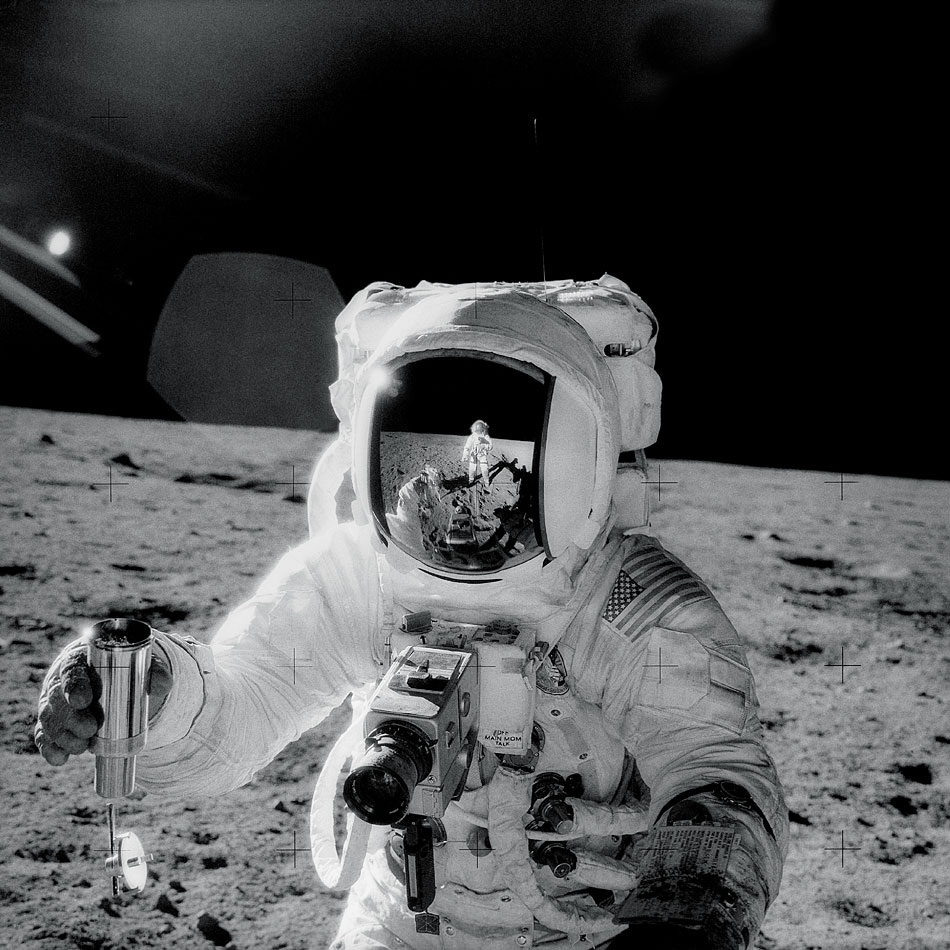
\includegraphics[width=0.8\textwidth]{images/bean_conrad_full.jpg}
\caption{\label{fig:bean}Astronaut Alan Bean on a lunar EVA during Apollo 12. The photographer, astronaut Pete Conrad, can be seen in Bean's helmet. Note Bean's left wrist, which sports a printed EVA timeline with notes about the tasks the crew needed to perform. \emph{Credit: Charles ``Pete'' Conrad, Apollo 12, NASA}.}
\end{figure}

\begin{figure}[htbp]
\centering
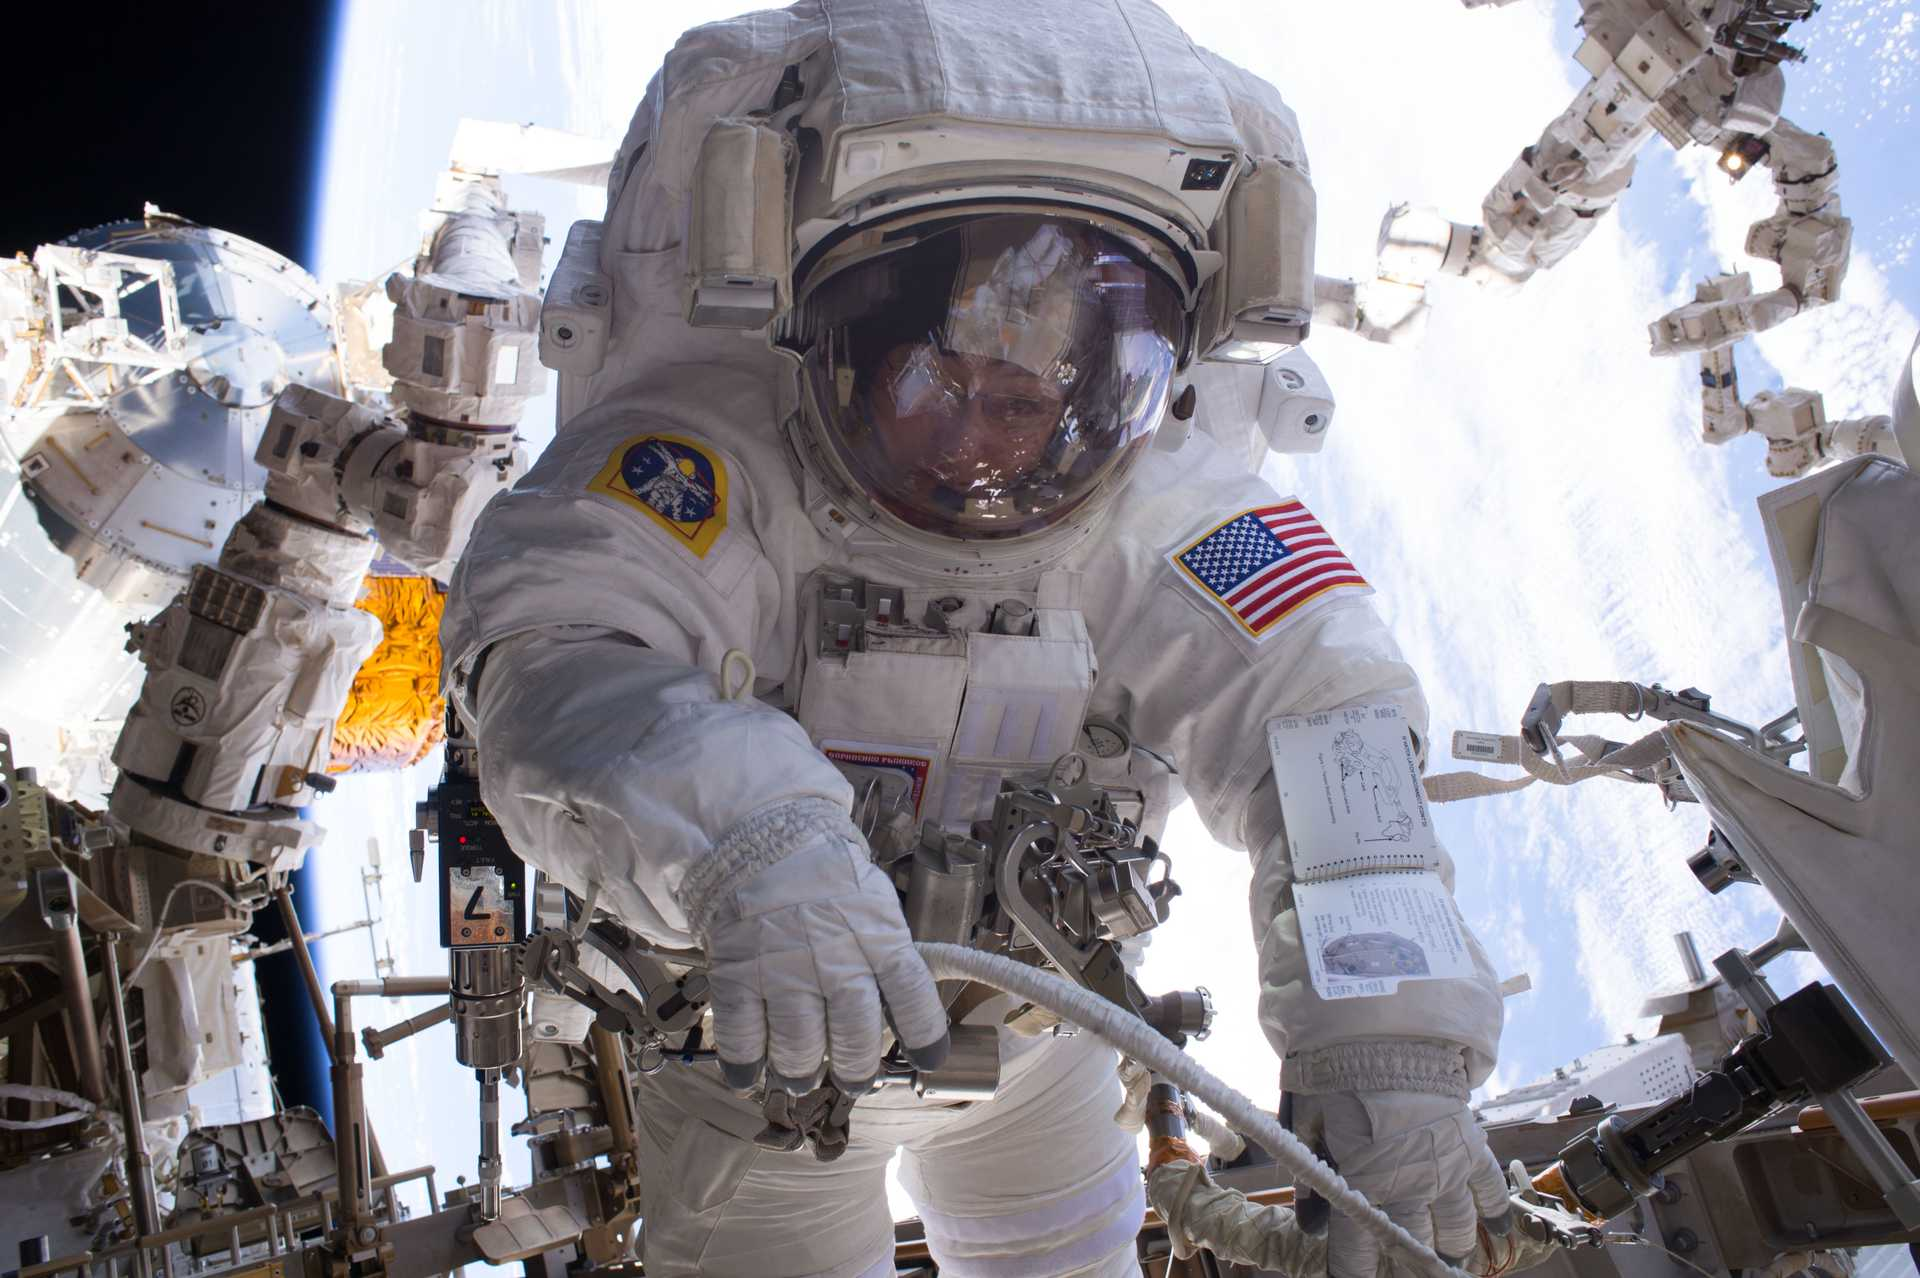
\includegraphics[width=0.8\textwidth]{images/whitson_full.jpg}
\caption{\label{fig:whitson}Astronaut Peggy Whitson on an ISS EVA in 2017. Note her left wrist, which sports a printed EVA timeline with notes about the tasks the crew needed to perform. \emph{Credit: NASA (\href{https://www.nasa.gov/image-feature/astronaut-peggy-whitson-during-a-spacewalk}{source})}.}
\end{figure}

\begin{figure}[htbp]
\centering
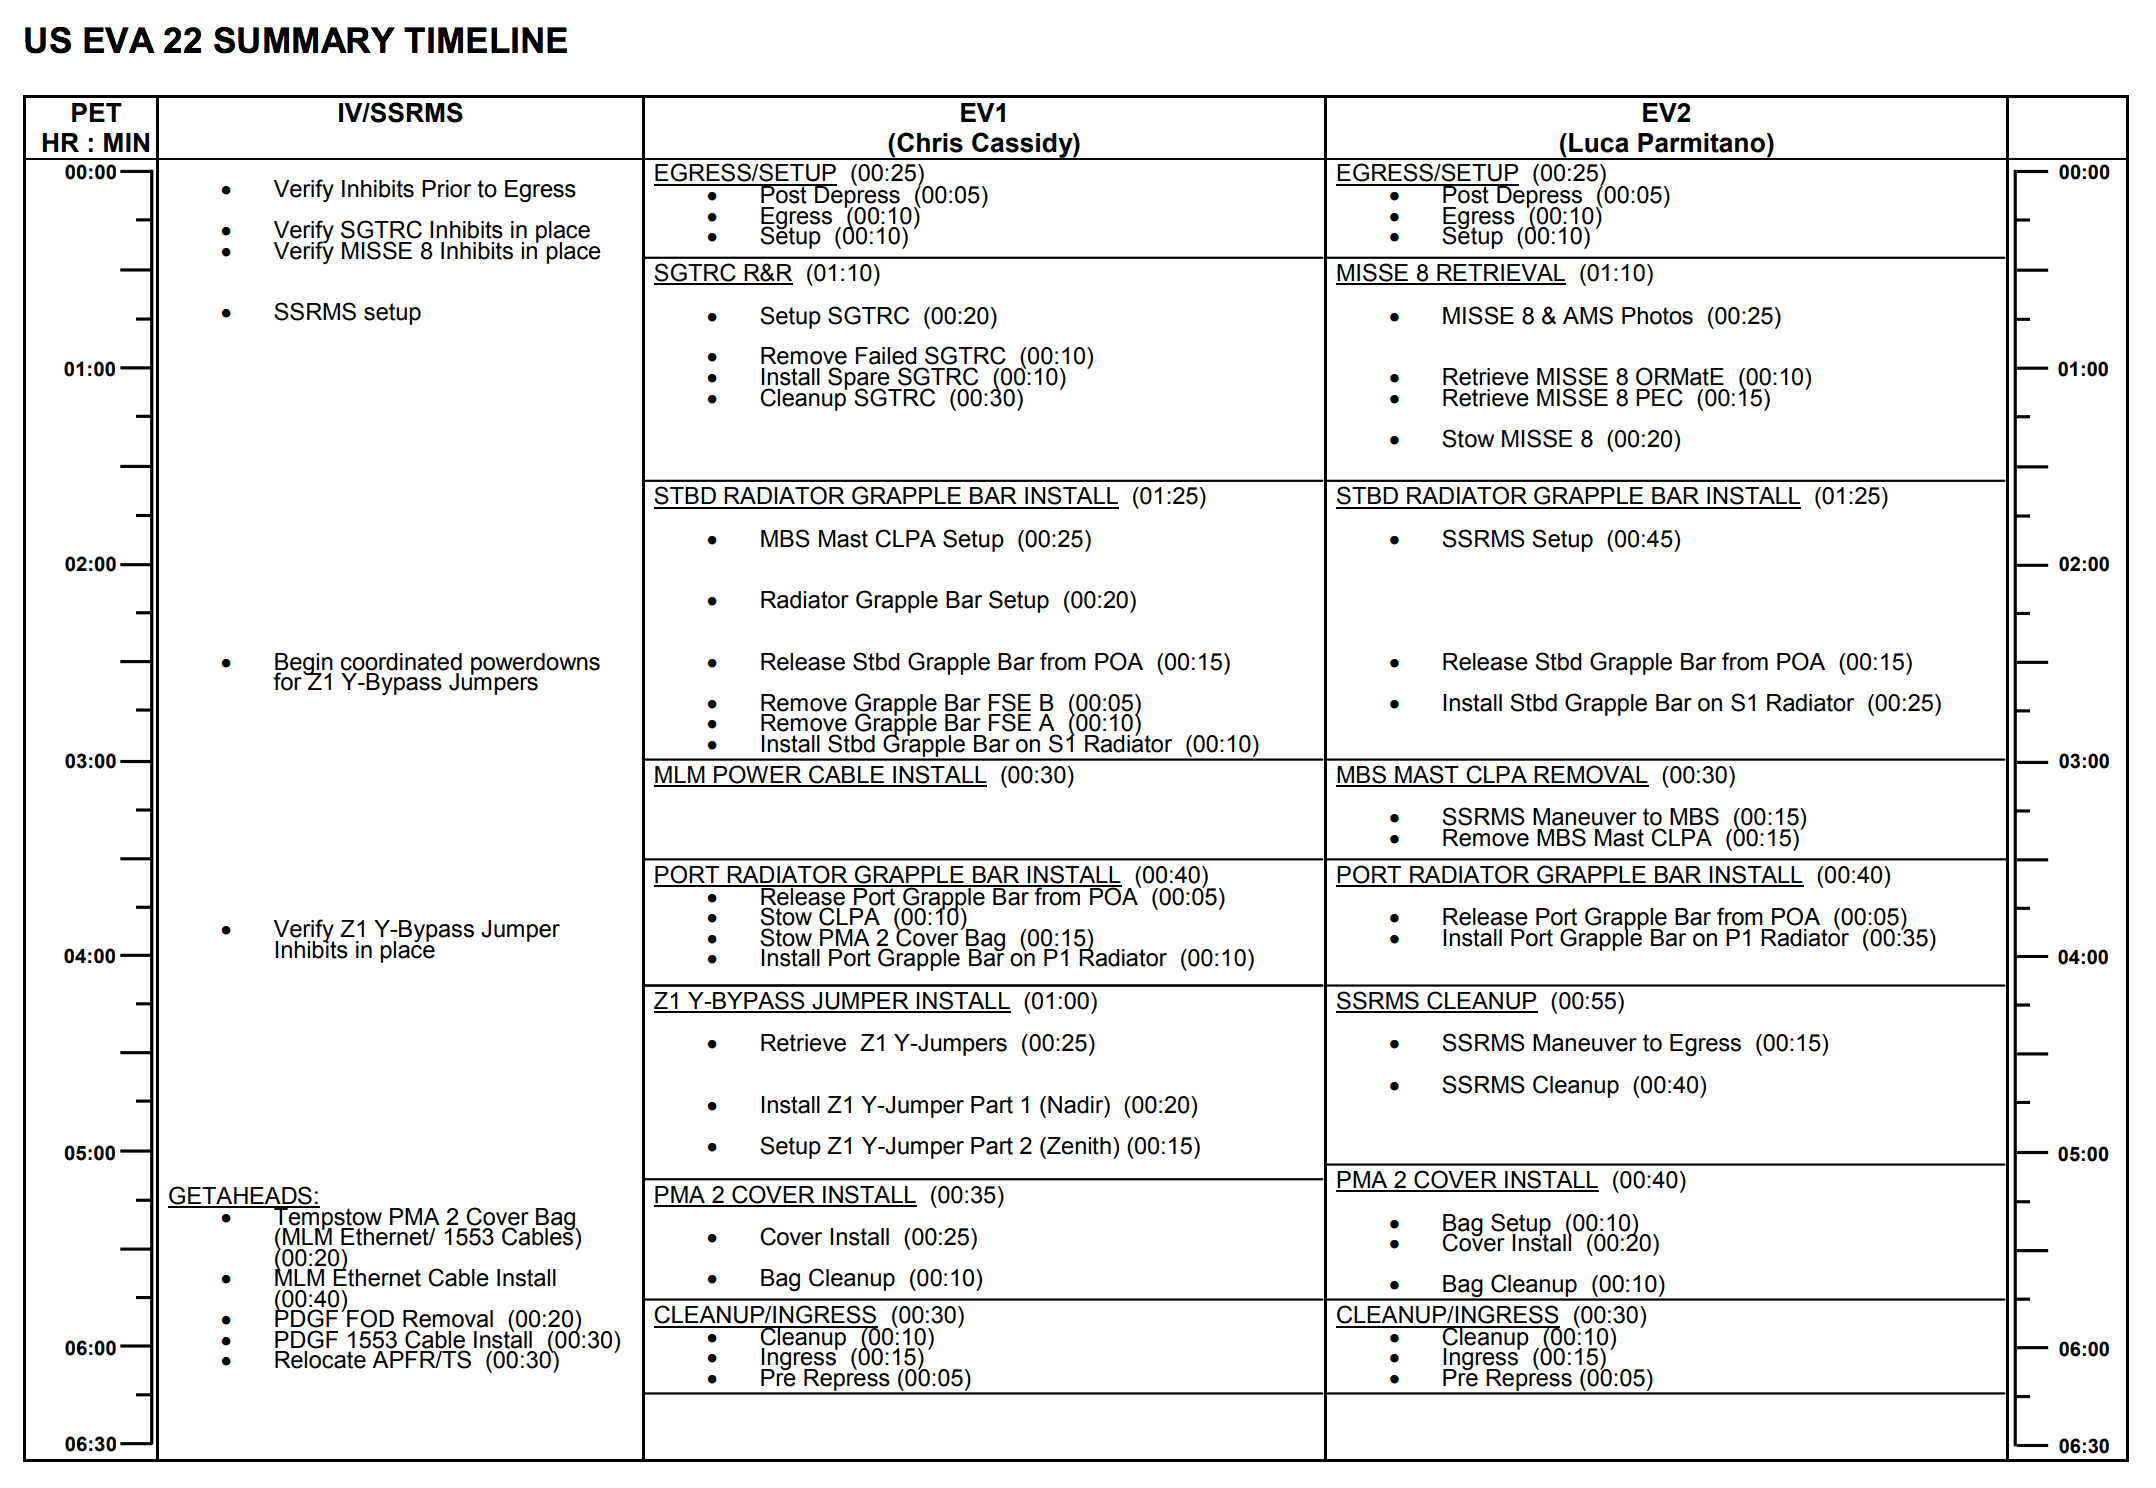
\includegraphics[width=\textwidth]{images/eva-timeline.png}
\caption{\label{fig:eva-timeline}The summary page from US EVA 22 on ISS. Each column represents a different agent with time increasing from top to bottom. ``PET'' is the Phased Elapsed Time, or time since the EVA began. Each activity has a time in HH:MM seconds associated with it. SSRMS is the Canadarm. EV1 and EV2 are the two spacewalkers. \emph{Credit: NASA (\href{https://www.nasa.gov/sites/default/files/files/US\%5fEVA\%5f22\%5fTimeline.pdf}{source})}}
\end{figure}

Of course, astronauts never work alone. In addition to communicating with MCC, crews perform EVAs on
a buddy system, meaning two crew members egress and ingress at the same time. At any given moment,
they may be collocated, distant, working independently, or in tight cooperation. Robotic assets also
play a role. On ISS, crews work with manipulators like the Canadarm \citeprocitem{8}{[8]}. Rovers and
robotic systems will almost certainly be present on the Moon. They may \emph{collaborate} in many ways.
Fundamentally, collaboration is a process of deciding when to perform actions based on when other
agents acted. For instance, taking a picture is a form of collaboration. In Figure \ref{fig:bean}, Pete
Conrad clearly decided when to snap a photo by observing when Alan Bean held up the sample
container. Maybe Conrad saw Bean getting ready and knew when to act. Or, more likely, Bean told
Conrad over the radio that he was ready for a picture, so Conrad should get the camera ready. We
envision that future digital assistants must facilitate similar collaboration. To do so, each agent
will have their own assistant, each running a scheduler that can reason over timing constraints
between their actions and the actions of their peers.

The gap in the current state of the art is that, to the best of our knowledge, there is no such
scheduler that is capable of reasoning over the sources of uncertain communication and observation
delay. Existing schedulers assume instantaneous communications, which is unreasonable on the lunar
surface, or indeed, any extreme environment. Furthermore, state of the art schedulers do not provide
collaborative capabilities that allow multiple agents to work together, especially in the presence
of uncertain communication. This thesis leverages and contributes to temporal reasoning research to
implement such a scheduler for multi-agent (MA) collaboration with uncertain communication, which we
refer to as a \emph{delay scheduler}.




For the remainder of the introduction, we present a short summary of each chapter.

\section{Problem Statement}
\label{sec:org44f37fa}

A delay scheduler can be used in the case of both one agent (e.g. a single astronaut or a robot)
working individually, as well as when multiple agents are collaborating. We start by defining the
problem statement for the single-agent case, before identifying the features that are necessary for
the MA case.

We use tools from temporal reasoning, namely temporal networks \citeprocitem{9}{[9]}, to model EVA
timelines as constraints (relationships) between a finite set of events. Some events are under an
agent's control, while others are not. Some events may have associated uncertain observation delay.

At some time \(t\) during an EVA, we have a set of events that were \emph{observed} before \(t\). When an
event has been recorded at \(t\), we say that it has been \emph{assigned}. If there is no associated
observation delay with an event, then the time of an observation is the same as assignment. If there
is associated observation delay, then it is possible that assignment times are earlier than their
respective observations.

We want a \emph{Real-Time Execution Decision} (RTED), which consists of unexecuted events and when they
should be performed. Each RTED consists of a set of unexecuted events to be scheduled at a future time.

Our problem statement for the delay scheduler is as follows. For some time \(t\) during scheduling,
the delay scheduler should take a temporal network, observation delay, observations thus far, and
assignments so far as input. It should output an RTED.

We expand the previous problem statement to the multi-agent case by adding the notion of agents.
Each agent has their own delay scheduler. As such, each delay scheduler receives a temporal network.
A subset of all events in their temporal network will be received from their peers in the form of
communications. From the perspective of an agent, their peers simply need to be aware of what events
have been assigned. Events that an agent receives from peers are no different than observations.

To be clear, each agent needs their own temporal network. In the EVA domain, we see the same
separation in Figure \ref{fig:eva-timeline} where each agent in the EVA has its own set of actions to
perform. While some actions are aligned between agents, there is no assumption that all agents are
working against the same events with the same constraints.

Thus, the multi-agent addition to the problem statement follows. Given event assignments and a set
of peers, all assignments made at \(t\) should be immediately communicated to all peers.

\section{Approach}
\label{sec:orgcf06beb}

The architecture of the delay scheduler is designed around the notion of taking everything we know
about set of temporal constraints and when events have been assigned and distilling it down to a
single RTED. There are three key processes in the delay scheduler.

\begin{enumerate}
\item an offline process that initializes the scheduler with a given model, including the temporal network
and observation uncertainty,
\item an online process that updates the scheduler with event assignments,
\item an online process that broadcasts event assignments with peers, and
\item an online process that queries for RTEDs.
\end{enumerate}

\begin{figure}[htbp]
\centering
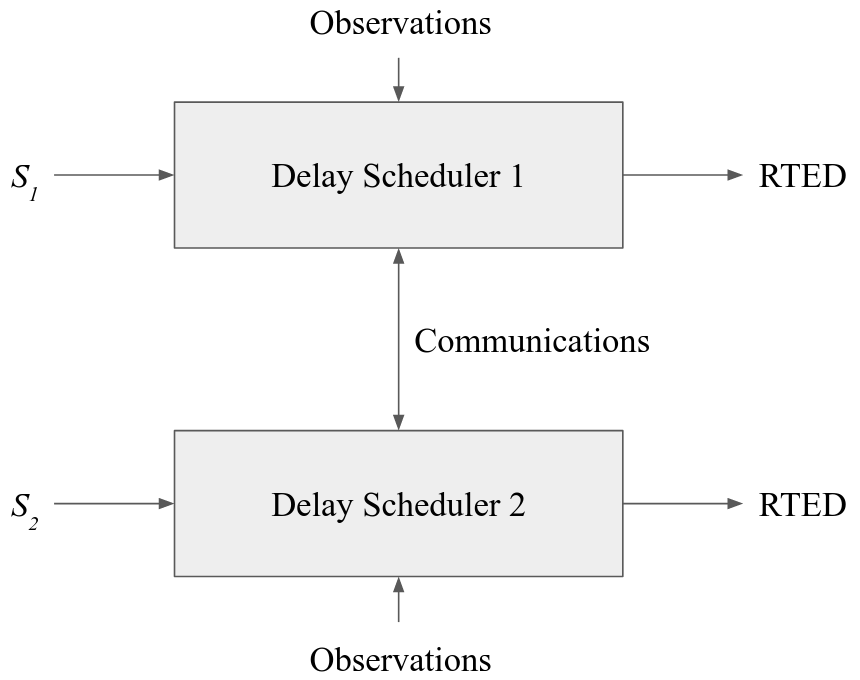
\includegraphics[width=0.7\textwidth]{images/approach-ma-schedulers.png}
\caption{\label{fig:intro-ma-schedulers}A sample architecture with two delay schedulers collaborating. Each agent receives a single temporal network as input. Observations of the outside world are recorded. Communications relay event assignments to peers. Each agent outputs its own RTED.}
\end{figure}

Much like how a flight controller cannot provide guidance on an EVA timeline without an accurate
copy of the EVA timeline, before scheduling begins, the scheduler must be given a model of the
schedule. Such a model will be unique to a given agent and must include all events, the constraints
between events, and the observation delay associated with events. Figure \ref{fig:intro-ma-schedulers}
represents this input as a separate model given to each scheduler offline.

During scheduling, schedulers receive observations of events. For a given agent, \(a\), observations
come from three sources: actions \(a\) has sensed but not controlled (``I traversed difficult terrain
and reached the installation location at \(t = 5\)''), actions \(a\) has performed (``I put the tripod
down at \(t = 6\)''), and actions that have been communicated to \(a\) (``It is \(t = 15\) and my peer told
me their confirmation arrived''). Figure \ref{fig:intro-ma-schedulers} shows observations coming from
outside the two schedulers while communications are passed between them.

As scheduling progress, a digital assistant will want to ask the scheduler for guidance as to when
to act. We represent the delay scheduler's output as an RTED, which can also be seen in Figure
\ref{fig:intro-ma-schedulers}.

\begin{figure}[htbp]
\centering
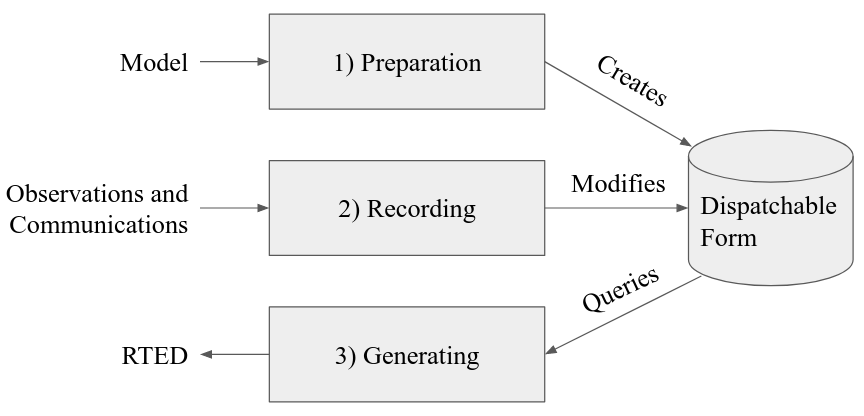
\includegraphics[width=0.7\textwidth]{images/approach-interfaces.png}
\caption{\label{fig:intro-interfaces}The four interfaces of a delay scheduler. The first is for initialization, the second is for schedule updates, the third is for broadcasting, and the fourth is for generating RTEDs. The dispatchable form is ultimately the source of truth for when events should be scheduled.}
\end{figure}

With three distinct processes involved in single-agent scheduling (subprocesses 1, 2, and 4), we
naturally define three explicit interfaces on the delay scheduler. Figure \ref{fig:intro-interfaces} shows
the flow of information between the interfaces and introduces a new data structure called the
\emph{dispatchable form}. In the context of scheduling, the dispatchable form is a graph structure that
acts like a database. Event assignments are recorded to the dispatchable form, and the dispatchable
form can be queried to find the next RTED. Note that Figure \ref{fig:intro-interfaces} is a
simplification. The dispatchable form is the key data structure that make scheduling possible, but
an implementation of a scheduler will store forms of data other than the dispatchable form when
events are recorded.

Importantly, the second interface in Figure \ref{fig:intro-interfaces}, recording, takes both
observations and communications as input. A key idea for the delay dispatcher is that communications
from agents are no different than event observations. Peer schedulers communicate when they have
assigned events, which then received as observations. We shall see that equating communications and
observations allows us to define a single-agent delay scheduler that can be seamlessly integrated in
a multi-agent context.

To enable communications between agents, delay schedulers are networked such that there is a
communication pathway between all agents. We do not assume every agent can communicate with ever
peer, rather when communications are received, they are relayed to all known peers.

\section{Modeling Temporal Constraints with Uncertain Observations}
\label{sec:org61dc494}

As stated before, our choice for modeling the ``what'' and ``when'' of scheduling is a temporal network,
also called a temporal constraint network \citeprocitem{9}{[9]}.

Temporal networks consist of events and constraints. Written in English, events and constraints
might be stated as ``samples must be stowed no more than five minutes after being collected.'' In this
case, \texttt{sample-collecting} and \texttt{sample-stowing} would be two events. It is the case that mission
planners have a robust set of modeling tools for creating schedules. In the literature, there are
constraints between events we can control \citeprocitem{9}{[9]}, events we cannot control
\citeprocitem{10}{[10]}, constraints between multiple agents \citeprocitem{11}{[11]}, events that may not be
observed \citeprocitem{12}{[12]}, and events with variable observation delay \citeprocitem{13}{[13]}. We
highlight key components of our chosen modeling framework below.

Our choice of modeling constraints is set-bounded ranges. That is, a constraint between two events,
``sample collecting'' and ``sample stowing'' is represented as
\(\edge{\texttt{sample-collecting}}{\texttt{sample-stowing}}{[0, 5]}\). \texttt{sample-stowing} must be
scheduled no earlier than \(0\) time units beforee and no later than \(5\) time units after
\texttt{sample-collecting}. This constraint assumes both \texttt{sample-collecting} and \texttt{sample-stowing} are under
the astronaut's full control. Perhaps the astronauts are working separately with one sample
collection bag shared between them. In that case, an astronaut might need to wait for their buddy to
finish using the bag before stowing samples. If so, then \texttt{sample-stowing} is outside their control.
We would then model the constraint as, say,
\(\conedge{\texttt{sample-collecting}}{\texttt{sample-stowing}}{[0, 5]}\). Now, the constraint
dictates that \texttt{sample-stowing} will happen no later than five minutes after sample collection, but
the astronaut cannot choose (control) when in the next five minutes \texttt{sample-stowing} is
scheduled.

Our choice of model for uncertain communication is variable observation delay \citeprocitem{13}{[13]}.
Say there is uncertain communication between the astronauts. Now the communication indicating that
\texttt{sample-stowing} can be begin may arrive either immediately, or a minute after it was sent. We model
the delay using a \emph{variable-delay function}, \(\gammabar(\texttt{sample-stowing}) = [0, 1]\).
Altogether, the astronaut may receive the communication indicating that \texttt{sample-stowing} may begin
instantaneously, or with up to a minute of delay. Key to our model is that the receiver \emph{does not
know how much a message was delayed}. If the message is received at \(t = 4\), then the communication
may have been sent at \(t = 4\) and received immediately. Or it is possible that it was sent as early
as \(t = 3\) and received after a minute delay.

Temporal networks play two key roles in scheduling. First, they allow a modeler to represent the
events and constraints between events of a schedule in a form that a scheduler can ingest. Second,
they can be checked for \emph{controllability} (also called \emph{consistency}). In order for it to be
possible for a temporal network to be scheduled, there must be a set of assignments for all events
under the agents control that satisfies all constraints in spite of the fact that some events may
arrive late or never at all.

With our choice of modeling constraints with variable observation delay, we perform a
\emph{variable-delay controllablity} check on temporal networks passed to the delay scheduler. A key
aspect of checking controllability is that we must the temporal network to one with less uncertainty
that is equivalent with respect to controllability. It is this less uncertain form of the temporal
network that we then schedule.

\section{Scheduling Events Despite Uncertain Observations}
\label{sec:org644c797}

From this point forward, we assume that the scheduler has been given a controllable temporal
network that accurately models the world.

Other researchers have presented single-agent scheduling algorithms for temporal networks with
uncontrollable events \citeprocitem{14}{[14]}, \citeprocitem{15}{[15]}, the fastest being FAST-EX
\citeprocitem{15}{[15]}. An underlying assumption of existing schedulers is that events are observed
instantaneously, that is \(\obs(x_{c}) = \assign(x_{c})\) for some uncontrollable event \(x_{c}\).
Events with uncertain observations are incompatible with this assumption, necessitating a change to
the way observations are recorded. The delay scheduler is a modified version of FAST-EX.

In fact, there are broadly two key differences between a delay scheduler and a scheduler that
implements FAST-EX. First, we must account for observation delay when events are observed. For
instance, if we know an observation at time \(t\) was delayed by \(\gamma\) time units, the assigned
time is then \(t - \gamma\). Second, we introduce a new variable to RTEDs, a \emph{no-operation}, or
\texttt{no-op}, boolean. Some events in an RTED may be \texttt{no-op} for reasons explained below.

When we transform the original temporal network with uncertain observations to one with less
uncertainty, we artificially shrink some of the constraints in the original temporal network. Some
uncontrollable events may arrive earlier or later than expected. We address these situations with
\emph{buffering} and \emph{imagining} uncontrollable events. We use the \texttt{no-op} addition to RTEDs to simplify
the handling of events that must be buffered or imagined.

\begin{figure}[htbp]
\centering
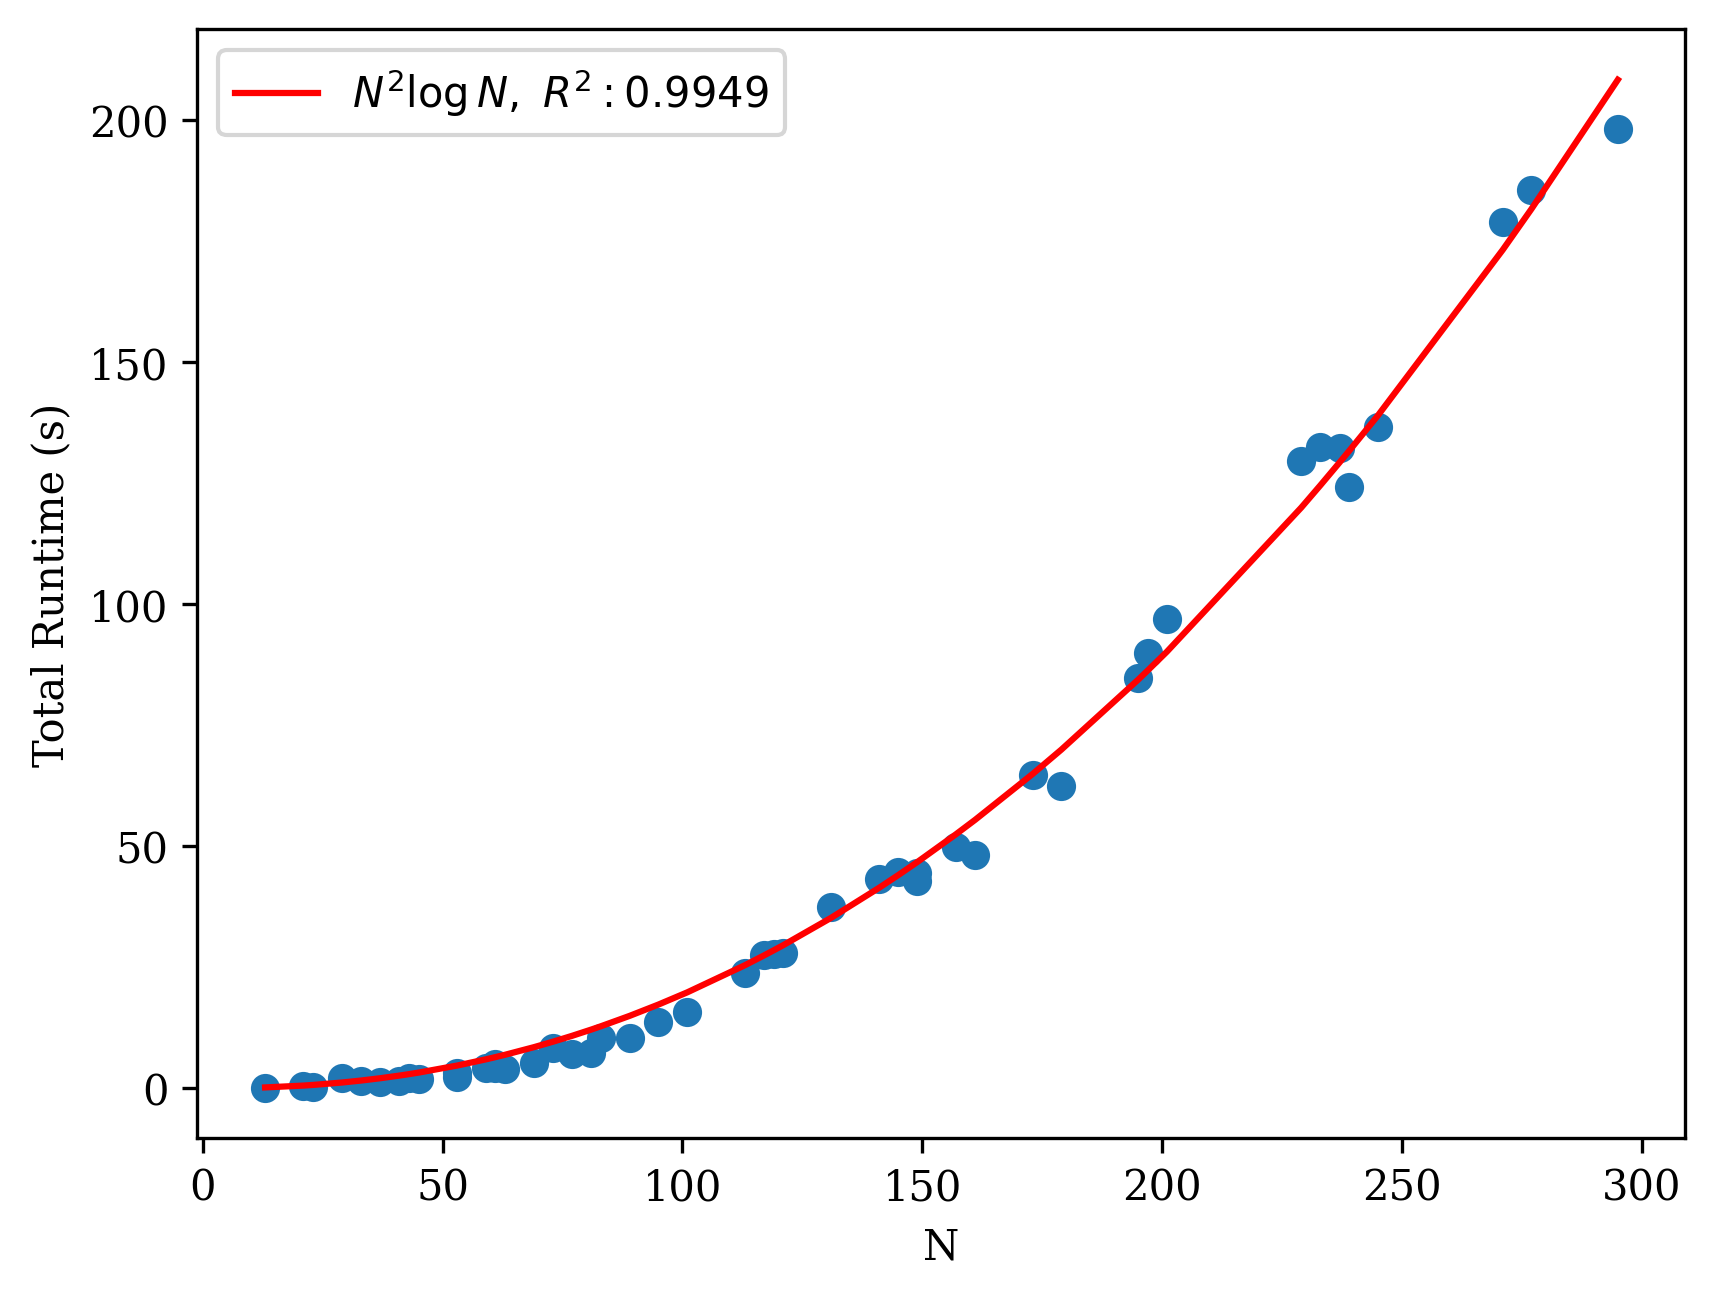
\includegraphics[width=0.8\textwidth]{images/scheduling-total-runtime-sub-300.png}
\caption{\label{fig:intro-runtime-scheduling}Total runtime data for scheduling all events in temporal networks with uncertain observations with less than 300 events.}
\end{figure}

We demonstrate that the delay scheduler exhibits the performance characteristics of FAST-EX. At the
core of FAST-EX is a Dijkstra Single Sink/Source Shortest Paths subroutine, which limits the runtime
performance. Each call to the subroutine should have a runtime performance of \(O(N \log N)\), where
\(N\) is the number of events in the temporal network. Thus, we expect the total runtime to schedule
all events in a temporal network to be \(O(N^{2} \log N)\). To evaluate the performance of the delay
scheduler, we scheduled randomly generated temporal networks with a structure inspired by a
satellite dish installation procedure. In the experiments, we model multiple astronauts (up to
eight) working in parallel with inter-agent temporal constraints. Figure
\ref{fig:intro-runtime-scheduling} shows that the delay scheduler demonstrates the expected performance
characteristics against said temporal networks.

\section{An Envisioned Executive for Dispatching Actions with Uncertain Observations}
\label{sec:org6405b6c}

We need a means to connect the RTEDs of a delay scheduler with the actions an agent performs. We
envision that the delay scheduler can serve as the scheduling logic behind an astronaut's digital
assistant, or in the case of a robot, a \emph{task executive}. A task executive should allow a human
modeler to provide constraints as input. The task executive is then charged with generating a plan
and dispatching actions as output.

We integrate the delay scheduler into a high-level task planner known as \emph{Kirk}. We call our variant
of Kirk, \emph{Delay Kirk}. A simplified overview of Delay Kirk's architecture can be found in Figure
\ref{fig:intro-kirk-architecture}. Delay Kirk takes the Reactive Model-Based Programming Language (RMPL)
\citeprocitem{16}{[16]}, a high-level language for modeling hybrid automata and constraints, as input. It
then creates a temporal plan network and chooses timed actions to execute to satisfy all the goals
as specified in RMPL. It is at this point that the delay scheduler can be integrated into delay
Kirk. With events and temporal constraints between them, the delay scheduler can produce RTEDs and
tell Delay Kirk when to act.

\begin{figure}[htbp]
\centering
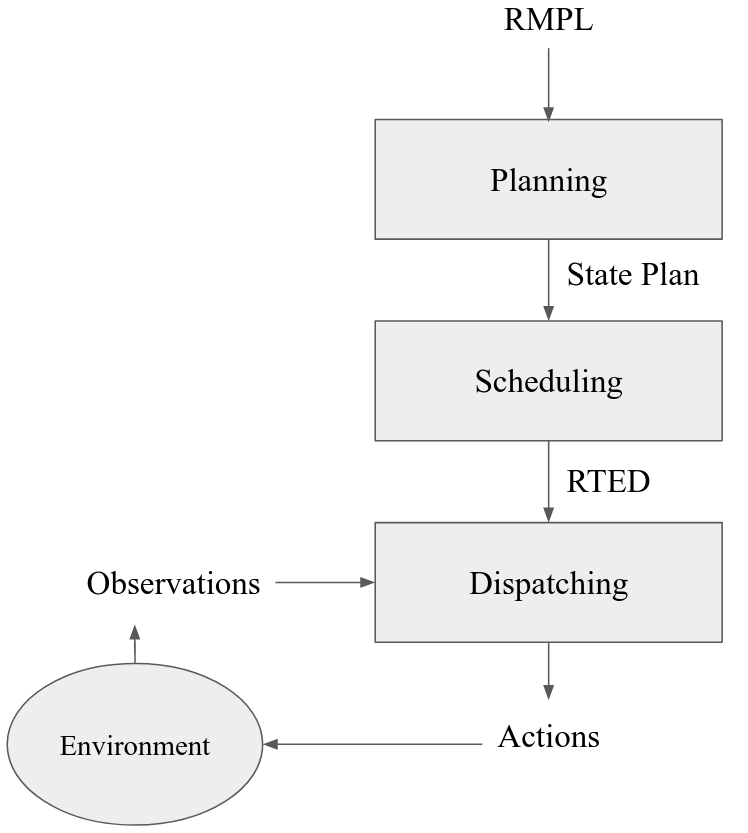
\includegraphics[width=0.6\textwidth]{images/executive-architecture.png}
\caption{\label{fig:intro-kirk-architecture}A high-level overview of the Delay Kirk task executive architecture with respect to dispatching actions.}
\end{figure}

For the purpose of this thesis, planning is out of scope. Instead, we focus on the \emph{delay
dispatcher} a component that enables an executive to impact an environment by taking actions based
on the RTEDs the delay scheduler produces.

\begin{figure}[htbp]
\centering
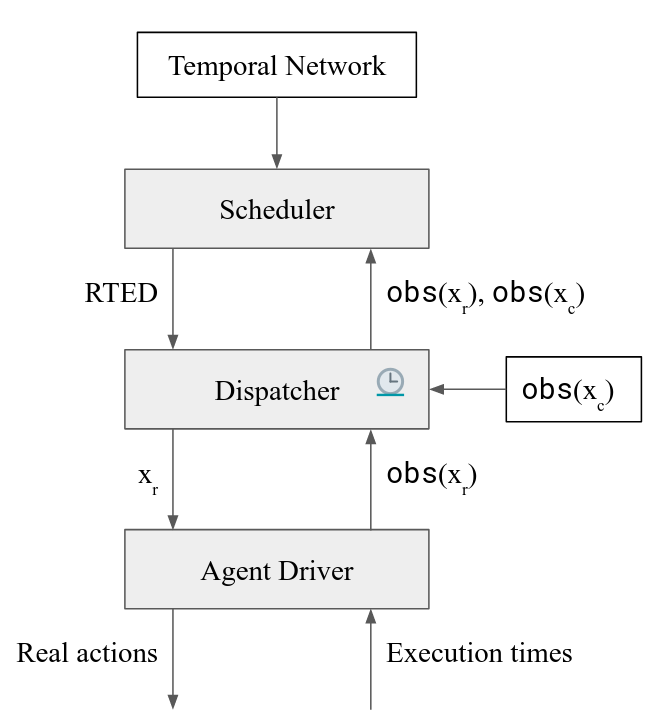
\includegraphics[width=0.6\textwidth]{images/architecture.png}
\caption{\label{fig:intro-dispatching-architecture}A more detailed view of the delay dispatcher architecture.}
\end{figure}

In Figure \ref{fig:intro-dispatching-architecture}, we introduce a new component, the \emph{driver}. We also
define new variables in order to paint a complete picture of the role the delay dispatcher plays.
\(x_{r}\) represents a controllable event. \(\obs(x_{r})\) and \(\obs(x_{c})\) represent the times that
controllable and uncontrollable events are observed respectively. The actions that the dispatcher
dispatches are mediated through the driver. Essentially, it translates events to commands that cause
actions to happen in the real-world. For a digital assistant, a driver might send a command to
update the heads-up-display in the crew's helmet. For a robot, the driver might publish a ROS
message \citeprocitem{17}{[17]}.

Note also that Figure \ref{fig:intro-dispatching-architecture} presents a different relationship between
the scheduler and observations, which are now passed to the scheduler through the dispatcher. We do
so because in our architecture the dispatcher, not the scheduler, has access to a clock. The
dispatcher takes the responsibility of comparing RTEDs to the clock time and deciding when to act.
Likewise, when events are observed, the dispatcher tells the scheduler when they were observed. This
change has the cumulative effect of giving the dispatcher responsibility for interacting with the
environment.

A key distinction between a normal dispatcher and the delay dispatcher is that not all observed
events are scheduled immediately. if an event should be buffered to a later time, then the
dispatcher has the responsibility of actually waiting until the correct clock time to record the
time in the scheduler.

\begin{figure}[htbp]
\centering
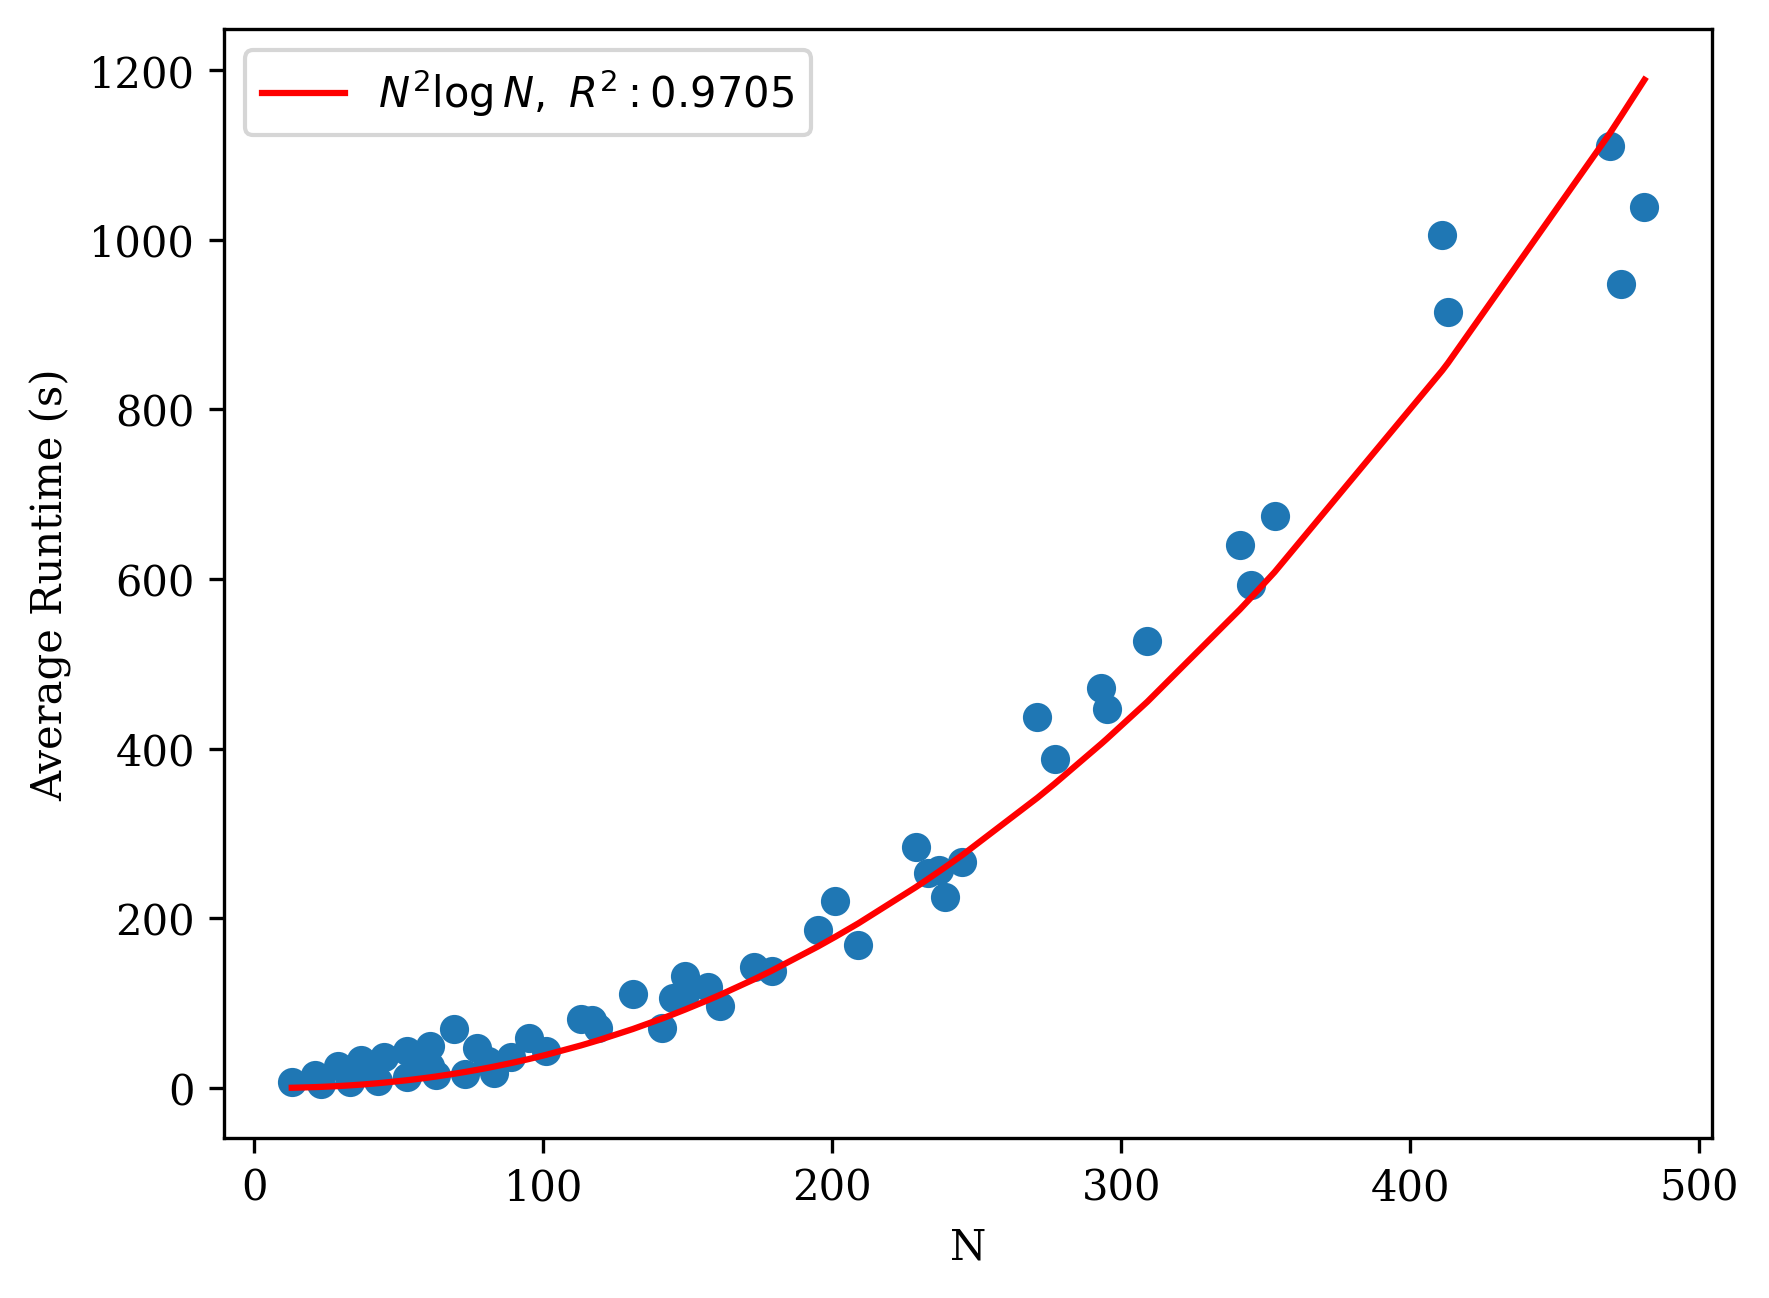
\includegraphics[width=0.8\textwidth]{images/tick-total-runtime.png}
\caption{\label{fig:intro-tick-runtime}A comparison of the total runtime to run the dispatcher against the number of events in a temporal network.}
\end{figure}

We evaluate the dispatcher's interface that loops and compares the clock time to an RTED to decide
when to act. For this tests, we use the same randomly generated temporal networks as were used when
evaluating the scheduler. Figure \ref{fig:intro-tick-runtime} shows the total runtime for all calls to the
dispatcher while scheduling all events in a temporal network. The Dijkstra updates that are
performed when recording events dominates the runtime performance. Given every event is recorded
inside this loop, we see the same \(O(N^{2} \log N)\) performance we saw when looking at the total
time to run all schedule updates.

\section{Multi-Agent Scheduling with Uncertain Observations}
\label{sec:orgeb3751a}

Collaboration between agents is enabled by enforcing that communications between agents are treated
the same as uncontrollable event observations. Thus, we are only challenged to define communication
pathways between agents that guarantee agents receive relevant observations. We do so by networking
delay schedulers in a \emph{communication graph}. A communication graph is a simple directed graph that
is used to broadcast event propagation messages between peers.

We evaluate the multi-agent delay scheduler in two simulations. In the first simulation, we run
three instances of Delay Kirk with inter-agent constraints between them. We compare their schedules
to the same schedule that would be produced if one delay scheduler tried to schedule all events for
all three agents. We found that the multi-agent delay dispatchers were able to schedule events while
respecting all inter-agent constraints.

\begin{figure}[htbp]
\centering
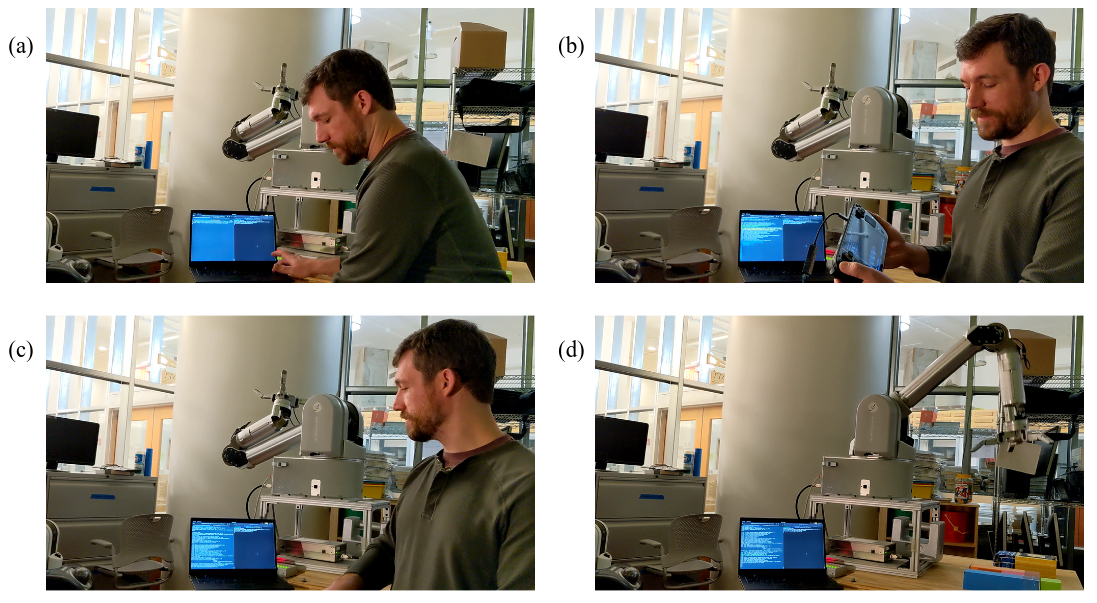
\includegraphics[width=\textwidth]{images/hw-demo-1-quad.png}
\caption{\label{fig:intro-hw-demo}A hardware demonstration in four parts. (a) \(t = 0\), when the two Kirks are started at the same time. (b) \(t = 16\), when the astronaut observed that the science experiment was setup. (c) \(t = 23\), when the robot received a delayed observation from the astronaut indicating they had completed science setup. (d) \(t > 23\), as the robot performed the drilling task.}
\end{figure}

We finally present a hardware demonstration with a Barrett WAM manipulator being controlled by one
Delay Kirk, with another Delay Kirk representing an astronaut's digital assistant. We demonstrate
that Delay Kirk is able to dispatch actions to the Barrett WAM while receiving communications
representing inter-agent constraints over HTTP.

\section{Thesis Structure}
\label{sec:org20210a1}

The structure of this thesis is as follows. A more detailed problem statement, including
descriptions of the scenarios used for testing distributed collaboration and coordination with
uncertain communication, will be provided in Chapter \ref{ch:problem-statement}. Our approach to
addressing the problem statement will be outlined in Chapter \ref{ch:approach}. Chapter \ref{ch:modeling-tn}
will provide the first technical contributions of this thesis, first by addressing the issue of
modeling observation delay, then by providing a procedure that can be used to guarantee that
temporal constraints with observation delay are satisfiable. Chapter \ref{ch:delay-scheduling} expands
existing algorithms for deciding when to act given the resolution of constraints. There, we
contribute a novel strategy for deciding when to act given observation delay. In Chapter
\ref{ch:technical-executive}, we formalize the components of task scheduling executive that can be
deployed to real hardware. Chapter \ref{ch:technical-coordination} finally contributes a multi-agent
coordination architecture for environments with uncertain communication. The discussion in Chapter
\ref{ch:discussion} concludes this thesis by providing additional context for the decisions made during
this research.

\chapter{Problem Statement}
\label{sec:orga6bb07c}
\label{ch:problem-statement}

There is a real-world need for coordinating multiple agents that are collaborating while facing
uncertain observations and uncertain inter-agent communication. We focus on an example drawn from
the domain of human spaceflight below, but any domain in which operations take place in extreme
environments needs to consider uncertain communication. Examples include military operations and
remote science, both summarized below.

For instance, military operators are frequently in environments where communication is impossible or
dangerous. Radioing from a staging area back to a command center may be impossible. Even
communications between operators in a hostile environment may risk exposing them to an enemy.
Despite communication concerns, there is an advantage for operations who can coordinate on a
battlefield. A delay scheduler would allow military operators to decide when to act given
uncertainty in their environment and communications.

Remote science with robotic explorers features many of the same communication and observation
constraints that are found in human spaceflight. The upcoming set of NASA Commercial Lunar Payload
Systems (CLPS) \citeprocitem{18}{[18]} rovers will be collecting samples and exploring the lunar
surface. While a CLPS rover is a single agent in and of itself, it is important to recognize that
both flight controllers and the scientists on the ground need to pass information between each other
and the rover to make the mission successful. From a scheduling perspective, CLPS mission execution
is a multi-agent scenario. The scientists and flight controllers running CLPS missions must contend
with uncertain or delayed communications. For example, there will likely be planned and unplanned
loss of signal events, uncertain delays in the arrival of scientific information due to protocols
like CFDP \citeprocitem{19}{[19]}, and issues with topological interference on the lunar surface.

Consider a subset of activities a rover might perform in a science station, or a small area where
multiple samples are collected. Within a tightly constrained window at each science station
(measured on the order of hours), a rover may collect core samples from multiple sites. Drill sites
within the science station might be pre-planned, however, it is possible that some later sites can
be changed by scientists based on the data collected so far. If that is the case, scientists would
have a limited time window after the first samples arrive to affect where later samples are
collected. A delay scheduler would allow the scientists to identify the last possible moment to
suggest a new drill site for the end of the science station, hence giving them as much time as
possible to analyze the data they receive and debate what other site might be most valuable. Without
taking communication delay into account, scientists may debate too long and miss an opportunity to
impact drill sites.

We now provide an example using EVAs to motivate the need for uncertain observations.

\section{EVAs as a Problem Domain}
\label{sec:orgcbb42e0}

EVAs must be performed in a timely manner. Life support imposes an upper bound on the total duration
of an EVA. As an EVA progresses, EV crews consume four non-renewable resources, comprised of oxygen,
battery power, water, and CO\(_2\) scrubbers \citeprocitem{20}{[20]}. The duration of EVAs is limited by
the consumable that is on track to be depleted first across the life support systems of both EV crew
members, referred to as the limiting consumable. Absent any other more pressing constraint, it is
this limiting consumable that forces EVA crews and ground support to stay on timeline.

Meanwhile, uncertain observations are manifested across three distinct categories: signal
transmission, human operational delays, and instrument processing. Each category presents a source
of delay that varies with uncertainty. For signal transmission, delay is sourced from the speed of
light between planetary bodies and infrastructural deficiencies. Communication infrastructure
outside of low-Earth orbit, including satellites and planetary surface signal repeaters
\citeprocitem{21}{[21]}, is not robust, and as such unpredictable delays and signal dropouts will be common
\citeprocitem{22}{[22]}. For human operational delays, note that the primary goal of Mission Control is
keeping the crew safe \citeprocitem{23}{[23]}. As such, communications from the science team to the crew
may be delayed or dropped because Mission Control needs to prioritize communications and actions
related to crew health and safety at the expense of science \citeprocitem{24}{[24]}, \citeprocitem{25}{[25]}. Lastly,
for instrument processing, there is uncertainty in the temporal relationships between the activation
of complex scientific instruments and the return of useful information \citeprocitem{26}{[26]}.
Scientific packages may generate high and low bandwidth data products, the uplink of which will be
bottlenecked by limited bandwidth between space and ground.

Consider a spacewalker who is installing an array of satellite dishes on the Moon. The procedure for
installing a single satellite dish is well defined. The procedure involves, say, firmly inserting a
tripod into the lunar regolith, putting a dish on top, bolting the dish in, attaching a few wires,
and waiting to get confirmation from ground that the dish is operational. Sometimes the tripod is
easy to burrow into the regolith, other times it takes a few tries. Sometimes the confirmation comes
quickly, other times it takes time. Some dishes are to be placed close to one another, yet others
should be far apart and across difficult to traverse terrain. Once one dish is done, the astronaut
can move on to the next. All the while, the astronaut's life support system is slowly draining its
consumable resources (e.g. oxygen and battery). Ground wants one dish tested at a time, so the
astronaut must wait for the confirmation before proceeding. But the astronaut also knows the
confirmation will come \emph{eventually}. They can continue to the next dish before receiving the
confirmation if they are confident that doing so still guarantees that the next installation will
not happen before the ground is ready. Another way of looking at it is that the astronaut knows
ground confirmed the installation, but the communication saying as much was delayed. The challenge
then is to wait as little time as necessary before moving on to the next dish. To decide when to
act, the astronaut relies on advice from the delay scheduler built in to their digital assistant.

\section{Problem Statement Definitions}
\label{sec:orgfd1232b}

Broadly speaking in this scenario, we have two types of input and one type of output. The first
input is decided before the astronaut egresses the habitat. MCC writes an EVA timeline (much like
Figure \ref{fig:eva-timeline}), which describes the events that need to take place and the relationship
between events, such as their ordering, the time between them, or how much delay there may be
between when an event occurs and when it is observed. Once the astronaut starts the EVA, we have a
second input, which is the time when events are observed. Taken together, we are tasked with finding
an output of deciding which future events should be executed at what time.

We use temporal networks \citeprocitem{9}{[9]} to model EVA timelines as temporal constraints between
a finite set of events. Some events may have associated uncertain observation delay. Let a temporal
network be represented by \(S\), which is a tuple of events \(X\) and constraints \(R\), \(\langle X, R
\rangle\). Constraints take the form of set-bounded intervals between two events. Some events in a
temporal network may be associated with an uncertain observation delay \(\gammabar\).

At some time \(t\) during an EVA, we have a set of events that were \emph{observed} before \(t\), \(\obs(x <
t)\). When an event has been recorded at a given time \(t\), we say that it has been \emph{assigned}. Both
observations and assignments are mappings from an event to a time in \(\mathbb{R}\).

The set of events that were assigned a time before \(t\) is \(\assign(x < t)\). If there is no
associated observation delay with an event \(x_{c}\), then \(\obs(x_{c}) = \assign(x_{c})\). If there is
associated observation delay, then it is possible that \(\obs(x_{c}) < \assign(x_{c})\).

We want a \emph{Real-Time Execution Decision} (RTED), which consists of unexecuted events and when they
should be performed. Each RTED is a tuple of a set of unexecuted events, \(x_{u} \subseteq X\) and
future time, \(t'\), \(\langle x_{u}, t' \rangle\).

Our specific problem statement for the delay scheduler is as follows.

\begin{defn}
\textbf{Single-Agent Delay Scheduler}

The delay scheduler should take triple \(\langle S, \gammabar, \obs(x < t) \rangle\) of the offline
(before scheduling) and online (during scheduling) components of scheduling as input. It must output
an RTED \(\langle x_{u}, t' \rangle\).
\end{defn}

We can expand the scenario from above to include multiple astronauts installing multiple satellite
dishes in parallel. MCC wants to minimize the number of dishes that are being confirmed at any given
moment. We add new \emph{inter-agent} constraints dictating that, given astronauts 1 and 2, astronaut 2
may not start installing a dish until they receive confirmation that astronaut 1 is complete.
Likewise, astronaut 3 must wait for 2 to finish their confirmation, 4 must wait for 3, and so on in
a round robin fashion. Like communication with MCC, communications between astronauts is spotty
(hence why they need to install communication infrastructure!) Sometimes, astronauts may easily
communicate, other times, communications may be significantly delayed or drop out altogether.
Naturally, the astronauts must be able to share events with each other to satisfy the inter-agent
constraints.

We expand the previous problem statement to the multi-agent case by adding the notion of agents,
\(A\), each with their own delay scheduler. Each delay scheduler has their own \(S_{a}\) with a subset
of events, \(x \subset X\), they expect to receive from their peers in the form of observations or
communications. While some actions are aligned between agents, there is no assumption that all
agents are working against the same events with the same constraints. From the perspective of an
agent, \(a \in A\), at time \(t\), their peers simply need to be aware of what events \(a\) has assigned
up to \(t\), \(\assign_{a}(x \leq t)\). Events that the peers of \(a\) communicate to \(a\) are no different
than observations of the environment that \(a\) makes.

We must define a problem statement for how delay schedulers should coordinate in a multi-agent
context.

\begin{defn}
\textbf{Multi-Agent Event Communications}

Given online input of tuple \(\langle \assign(x_{t}), A\), agent \(a\) should output all assignments
\(\assign_{a}(x_{t})\) in the form of a broadcast to all other agents, \(A - \{a\}\).
\end{defn}

In other words, event assignments should be broadcasted to all peers as soon as an assignment is
made.

\chapter{Approach}
\label{sec:orge8b7df2}
\label{ch:approach}

We define a delay scheduler in such a way that one instance is useful for single-agent scheduling,
and multiple instances can be seamlessly integrated for collaboration with inter-agent constraints.
Our approach builds towards such a multi-agent delay scheduler by first defining the subproblems
necessary for single-agent scheduling with uncertain communication before layering on a
communication pathway for multi-agent scheduling. Figure \ref{fig:approach-ma-schedulers} presents a
simplified view of multi-agent scheduling.

\begin{figure}[htbp]
\centering
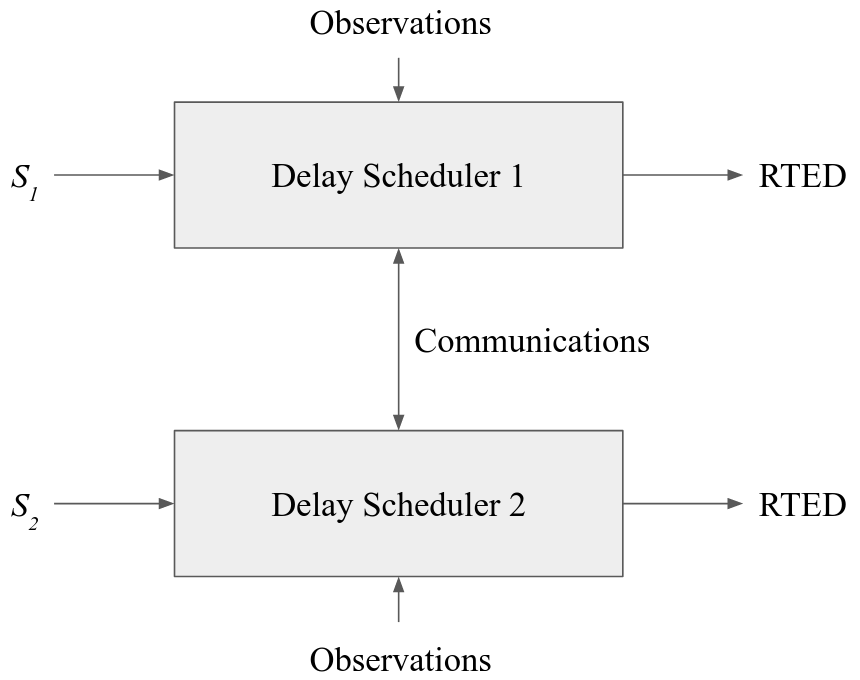
\includegraphics[width=0.7\textwidth]{images/approach-ma-schedulers.png}
\caption{\label{fig:approach-ma-schedulers}A sample architecture with two delay schedulers collaborating. Each agent receives a single temporal network as input. Observations of the outside world are recorded. Communications relay event assignments to peers. Each agent outputs its own RTED.}
\end{figure}

Our approach relies on the ability of a delay scheduler to accurately decide what events should be
scheduled and when it is \emph{valid} to do so. In this context, a decision being ``valid'' means that the
events and time of an RTED guarantees that all constraints in the problem can be satisfied given the
history of events scheduled before now. We naturally need one or more data structures that, if
maintained correctly during scheduling, can be queried to produce such an RTED. We refer to such a
data structure as the dispatchable form, though, as will be seen in Chapter \ref{ch:delay-scheduling},
other data structures facilitate scheduling as well.

A delay scheduler must be able to output RTEDs that are consistent with the constraints of the
problem and the history of scheduled events. There are four key subproblems that must be addressed:

\begin{enumerate}
\item an offline process must \textbf{initialize} a dispatchable form that reflects the semantics of \(S\) and
\(\gammabar\),
\item an online process must \textbf{update} the dispatchable form given an event observation at a given time,
\item an online process must \textbf{broadcast} new event assignments with peers, and
\item an online process must \textbf{query} the dispatchable form for new RTEDs.
\end{enumerate}

\begin{figure}[htbp]
\centering
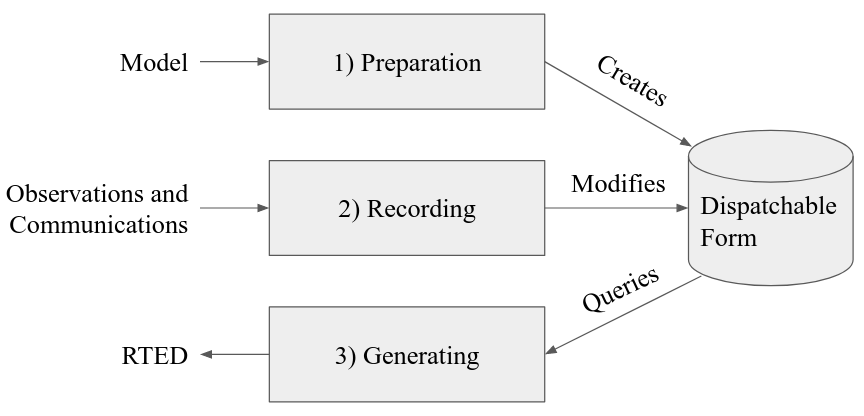
\includegraphics[width=0.7\textwidth]{images/approach-interfaces.png}
\caption{\label{fig:approach-interfaces}The four interfaces of a delay scheduler. The second and third are combined to highlight that broadcasts are trigged when events are observed. The first shows the dispatchable form being intialized from a model. The second shows that event observations will cause the dispatchable form to be updated, immediatelly triggering a broadcast (the third interface). The fourth interface queries the dispatchable form to create RTEDs.}
\end{figure}

Figure \ref{fig:approach-interfaces} shows the architecture of a delay scheduler with respect to its four
interfaces and dispatchable form.

\begin{algorithm}
\SetAlgoLined
\SetKwFunction{Return}{return}
\SetKwInput{Input}{Input}
\SetKwInput{Output}{Output}
\SetKwInput{Algorithm}{\textsc{Delay Scheduling}}
\SetKwInput{Initialize}{Initialization}
\SetKwIF{If}{ElseIf}{Else}{if}{then}{else if}{else}{endif}
\Indm
\Input{Controllable temporal network $S$; Observation uncertainty $\gammabar$; \texttt{clock}; \texttt{peers}}
\Initialize{\texttt{dispatchable-form} $\gets$ \texttt{initialize}($S, \gammabar$); \texttt{RTED} $\gets \varnothing$;}
\Indp
\Algorithm{}
\Indp

\While{there are unexecuted executable events} {
  \If{Event $x$ is observed} { \label{line:event-observed}
    \texttt{update(dispatchable-form, $x$, clock.now))}\;
    \texttt{broadcast($x$, peers)}\;
  }

  \texttt{RTED} $\gets$ \texttt{query(dispatchable-form, clock.now)}
}
\caption{Algorithm for performing delay scheduling to produce RTEDs for all executable events in a temporal network.}
\label{alg:approach-delay-scheduler}
\end{algorithm}

We provide pseudo-code for a delay scheduler in Algorithm \ref{alg:approach-delay-scheduler}. \texttt{initialize}
will create the dispatchable form, \texttt{update} will modify the dispatchable form to reflect an event
assignment, \texttt{broadcast} will send event assignments to peers, and \texttt{query} will read the dispatchable
form to find the next RTED.

For now, we make the following assumptions. We assume that initialization, updates, and queries are
sound and complete algorithms with respect to their intended handling of the dispatchable form. We
use the term ``networked'' to refer to agents that can communicate event observations to each other.
Broadcasting assumes the existence of a communication protocol that guarantees messages indicating
an event has been assigned reach all networked schedulers. If a temporal network is controllable,
then there must exist a dispatchable form \citeprocitem{27}{[27]}.

Below, we prove that Algorithm \ref{alg:approach-delay-scheduler} will guarantee the output of valid RTEDs
for all executable events for coordinating agents. We start by showing that the delay scheduler can
be used in a multi-agent context.

\begin{lemma}
\label{lemma:approach-all-controllable}
For \(a\) delay schedulers, if each \(S_{a}\) and \(\gammabar_{a}\) received by each delay scheduler \(a
\in A\) is controllable and accurately models the world, then all networked delay schedulers may
produce valid RTEDs.
\end{lemma}

\begin{proof}
If \(S_{a}\) is controllable for a single delay scheduler, then there must exist a set of RTEDs that
allows all constraints to be satisfied for all resolutions of uncertainty in the uncontrollable
constraints and observation delay. If it were not the case that any \(S_{a}\) and \(\gammabar_{a}\)
accurately models the world, then the uncontrollable inter-agent constraints of \(S_{a}\) and
\(\gammabar_{a}\) would not strictly encompass all possible outcomes of uncertainty during scheduling.
This would mean that, during scheduling, there may be a resolution of uncertainty that does not
allow a valid RTED to be produced, which is inconsistent with a controllable \(S_{a}\). Thus if each
\(S\) is controllable and accurate for all delay schedulers, then all delay schedulers may produce
valid RTEDs.
\end{proof}

We now show that the delay scheduler will produce valid RTEDs in a single-agent context.

\begin{lemma}
\label{lemma:initialization}
Given a controllable temporal network \(S\) consisting of a set of events, \(X\), constraints, \(R\), and
uncertain observation delay, \(\gammabar\), initializing the dispatchable form before the first event
is observed guarantees the dispatchable form can be used to schedule any executable event in \(X\).
\end{lemma}

\begin{proof}
As an offline process, by definition initialization will run before scheduling begins. Thus, the
dispatchable form must be valid and include enough information to schedule all executable events.
\end{proof}

Not all events may be observed. For instance, any event with infinite observation delay (as may
occur during a communication dropout) is unobservable. The delay scheduler cannot schedule events
with infinite observation delay.

\begin{lemma}
\label{lemma:observable-events}
All events that have the ability to impact RTEDs may be observed by the delay scheduler.
\end{lemma}

\begin{proof}
If \(S\) is controllable, then it must be the case that the delay scheduler can output RTEDs that will
guarantee all constraints between events can be satisfied. If it were the case that unobservable
events must be assigned in order to produce a valid RTED, then scheduling would depend on
information that cannot be learned, meaning \(S\) would not be controllable.
\end{proof}

For the next lemma, it is important to highlight that RTEDs may not depend on information about
future events.

\begin{lemma}
\label{lemma:all-events-are-observed}
If an event is scheduled, it will be observed by the delay scheduler.
\end{lemma}

\begin{proof}
There are two parts to this proof. First, the delay scheduler loops without pause until all
executable events have been scheduled, meaning that the conditional on line
\(\ref{line:event-observed}\) will be reached for all events that can have an impact on RTEDs.

Second, RTEDs are not the same as event assignments. As will be shown in Definition \ref{def:rted-op}, the
execution time of an RTED must be in the future. We are not allowed to assign an event to a future
time, thus the events in an RTED cannot be immediately scheduled. We observe when executable events
are scheduled in the future.
\end{proof}

\begin{lemma}
\label{lemma:observe-then-rted}
If we observe all events before producing RTEDs, then RTEDs will always be valid.
\end{lemma}

\begin{proof}
We see that we always check for event observations before producing RTEDs. There are no processes
between checking for an observation and producing an RTED. Therefore, each RTED will be queried
against a dispatchable form that has been modified to reflect all event assignments up to the
current time. If the choice of dispatchable form is valid for any set of assignments up to the
current time, and the querying process is sound and complete, then the RTED must also be valid.
\end{proof}

We finish by revisiting the multi-agent context.

\begin{lemma}
\label{lemma:approach-broadcasting}
If there are satisfiable inter-agent constraints, then broadcasting all event assignments to all
peers guarantees that each delay scheduler may produce valid RTEDs.
\end{lemma}

\begin{proof}
All observable events must be assigned. If all event assignments are broadcasted to all agents, then
it must be the case that all agents observe all events. If all observable events are received for a
controllable \(S\), then it must be the case that a delay scheduler can produce a valid RTED, and thus
all networked delay schedulers can produce valid RTEDs.
\end{proof}

The next chapters will address each of the assumptions made above. Chapter \ref{ch:modeling-tn} will
elaborate on modeling temporal networks with uncertain communication and checking their
controllability. Chapter \ref{ch:delay-scheduling} will focus on the process of creating and maintaining a
dispatchable form throughout single-agent scheduling. Chapter \ref{ch:technical-executive} describes the
integration of Algorithm \ref{alg:approach-delay-scheduler} in a high-level task executive. Chapter
\ref{ch:technical-coordination} will describe the design of a robust broadcasting algorithm for networked
schedulers with uncertain communication.

\chapter{Modeling Temporal Constraints with Uncertain Observation Delay}
\label{sec:org6b23468}
\label{ch:modeling-tn}

Our overarching aim in this Chapter is to architect the offline portions of a single-agent pipeline
that takes a temporal network with uncertain observation delay of exogenous events as input in order
to execute events in the real world within time windows that guarantee temporal consistency. Given
everything we know and do not know about the temporal relationship between events within and outside
of our control, this chapter will lay the groundwork that there exists an execution strategy that
guarantees all constraints are satisfied despite the uncertainty. The next chapter, Chapter
\ref{ch:delay-scheduling}, will provide accompanying online procedures for acting on said execution
strategy and dispatching events with real hardware (or by generally telling an agent what to do).

The three aims of this chapter are to

\begin{enumerate}
\item model temporal constraints with uncertain observation delay,
\item define a consistency (controllability) checking procedure for temporal networks with uncertain
observation delay, and
\item prove that the execution strategy assumed by the controllability checking procedure is safe.
\end{enumerate}

In Section \ref{sec:tn}, we address aim (1) by outlining the necessary definitions for modeling temporal
networks. Sections \ref{sec:fdc} and \ref{sec:vdc} describe our chosen model for temporal constraints with
uncertain observation delay, and address aim (2) by presenting a procedure for checking the
consistency thereof. Sections \ref{sec:fdc} and \ref{sec:vdc} are largely based on the work originally put forth
by Bhargava et. al., \citeprocitem{13}{[13]}, \citeprocitem{28}{[28]}, \citeprocitem{29}{[29]} with additional
contributions by us as highlighted below. Notably, Section \ref{sec:vdc} addresses aim (3) by contributing
novel proofs that the execution strategy assumed to exist by Bhargava et. al. is safe. We conclude
with experimental analysis of our chosen consistency checking procedure in Section
\ref{sec:vdc-experimental} using example temporal constraint networks inspired by lunar exploration.

\section{Temporal Networks}
\label{sec:orgb6ed869}
\label{sec:tn}

Temporal networks form the backbone of our architecture for temporal reasoning under observation
delay. Simple Temporal Networks (STNs) offer the basic building blocks for most expressive temporal
network formalisms \citeprocitem{9}{[9]}. An STN is composed of a set of variables and a set of binary
constraints, each of which limits the difference between a pair of these variables; for example,
\(B - A \in [10, 20]\). Each variable denotes a distinguished point in time, called an \emph{event}.
Constraints over events are binary \emph{temporal constraints} that limit their temporal difference; for
example, the aforementioned constraint specifies that event \(A\) must happen between 10 and 20
minutes before event \(B\).

\begin{defn}
\textbf{STN} \citeprocitem{9}{[9]}

An \emph{STN} is a pair \(\langle X, R \rangle\), where:
\begin{itemize}
\item \(X\) is a set of variables, called events, each with a domain of the reals \(\mathbb{R}\), and
\item \(R\) is a set of simple temporal constraints. Each constraint \(\langle x_r, y_r, l_r, u_r \rangle\)
has scope \(\{ x_r, y_r \} \subseteq X\) and relation \(x_r - y_r \in [l_r, u_r]\).
\end{itemize}
\end{defn}

\begin{defn}
\textbf{Schedule} \citeprocitem{27}{[27]}

A \emph{schedule}, \(\assign\), is a mapping of events to times, \(\assign : X \rightarrow \mathbb{R}\).
\end{defn}

An STN is used to frame scheduling problems. A schedule is feasible if it satisfies each constraint
in \(R\). We use the notation \(\assign(x)\) to represent a mapping from an event, \(x\), to a time, \(x
\rightarrow \mathbb{R}\), in the schedule. A schedule is \emph{complete} if all \(x \in X\) are assigned
times in \(\assign\). An STN is \emph{consistent} if it has at least one feasible schedule that assigns all
events in \(X\).

An STN is consistent if and only if there is no negative cycle in its equivalent distance graph
\citeprocitem{9}{[9]}. Let \(n\) be the number of events in a temporal network and \(m\) to be the number
of constraints. Then consistency of an STN can be checked in \(O(mn)\) time using the Bellman-Ford
Algorithm \citeprocitem{30}{[30]} to check for negative cycles.

While an STN is useful for modeling problems in which an agent can control the exact time of all
events, it does not let us model actions whose durations are uncertain. A Simple Temporal Network
with Uncertainty (STNU) is an extension to an STN that allows us to model these types of uncertain
actions \citeprocitem{10}{[10]}.

\begin{defn}
\label{def:stnus}
\textbf{STNU} \citeprocitem{10}{[10]}

An \emph{STNU} \(S\) is a quadruple \(\langle X_e, X_c, R_r, R_c \rangle\), where:
\begin{itemize}
\item \(X_e\) is the set of executable events with domain \(\mathbb{R}\),
\item \(X_c\) is the set of contingent events with domain \(\mathbb{R}\),
\item \(R_r\) is the set of requirement constraints of the form \(l_r \leq x_r - y_r \leq u_r\), where \(x_r,
  y_r \in X_c \cup X_e\) and \(l_r, u_r \in \mathbb{R}\), and
\item \(R_c\) is the set of contingent constraints of the form \(0 \leq l_r \leq c_r - e_r \leq u_r\), where
\(c_r \in X_c\), \(e_r \in X_e\) and \(l_r, u_r \in \mathbb{R}\).
\end{itemize}
\end{defn}

An STNU divides its events into executable and contingent events and divides its constraints into
requirement and contingent constraints. The times of executable events are under the control of an
agent, and assigned by its scheduler. STNU executable events are equivalent to events in an STN.
Contingent events are controlled by Nature. Contingent constraints model the temporal outcomes of
uncertain actions and are enforced by Nature. Contingent constraints relate a starting executable
event and an ending contingent event. To ensure causality, the lower-bound of a contingent
constraint is required to be non-negative; hence, the end event of the constraint follows its start
event. Contingent constraints are not allowed to be immediately followed by additional contingent
constraints. Requirement constraints specify constraints that the scheduler needs to satisfy and may
relate any pair of events. An STNU requirement constraint is equivalent to an STN constraint.

To clarify terminology, we sometimes refer to contingent constraints as contingent links and
requirement constraints as requirement links. We also sometimes use the term \emph{free} instead of
requirement to describe executable events and constraints. When we discuss contingent constraint or
contingent link duration, we refer to the amount of time that actually elapses between a contingent
link's starting executable event and its ending contingent event. We sometimes refer to STNUs as
defined in Defintion \ref{def:stnus} as \emph{vanilla} STNUs (in contrast to the many ``flavors'' of STNUs,
namely the variants with fixed and variable observation delay functions as will be defined in
Sections \ref{sec:fdc} and \ref{sec:vdc} respectively).

With STNs, our goal is to construct a consistent schedule for all events such that all constraints
are satisfied. In STNUs, however, contingent events cannot be scheduled directly. Instead, we are
interested in determining whether there is a \emph{controllable} execution strategy that guarantees that
a schedule can be constructed such that all constraints are satisfied despite how uncertainty is
resolved.

\begin{defn}
\textbf{Situations} \citeprocitem{10}{[10]}

For an STNU \(S\) with \(k\) contingent constraints \(\langle e_{1}, c_{1}, l_{1}, u_{1} \rangle, \cdots,
\langle e_{k}, c_{k}, l_{k}, u_{k} \rangle\), each \textit{situation}, \(\omega\), represents a
possible set of values for all links in \(S\), \(\omega = (\omega_{1}, \cdots, \omega_{k}) \in \Omega\).
The \textit{space of situations} for \(S\), \(\Omega\), is \(\Omega = [e_{1}, c_{1}] \times \cdots \times
[e_{k}, c_{k}]\).
\end{defn}

Each \emph{situation} in the \emph{space of situations}, \(\omega \in \Omega\), represents a different
assignment of contingent links in the schedule \citeprocitem{10}{[10]}. We may represent the situation for
a specific constraint as \(\omega_{i}\) for the i-th constraint in \(S\), or \(\omega(x_{c})\) for
contingent event \(x_{c}\).

Situations may be applied to STNUs.

\begin{defn}
\textbf{Projection} \citeprocitem{10}{[10]}, \citeprocitem{27}{[27]}

A \emph{Projection} is an application of a situation, \(\omega\), on an STNU \(S\), which collapses the
durations of contingent links to specific durations resulting in an STN.
\end{defn}

A \emph{projection} is an STN that is the result of applying a situation to an STNU, and thus the
contingent links have reduced from uncertain ranges to specific durations
\citeprocitem{10}{[10]}, \citeprocitem{27}{[27]}.

\begin{defn}
\textbf{Execution Strategy}

An \emph{execution strategy}, \(\mathcal{S}\), is a mapping of situations to schedules,
\(\mathcal{S}~:~\Omega \rightarrow \Xi\).
\end{defn}

An \emph{execution strategy} then naturally maps a specific resolution of the uncertainty of the
contingent constraints to a set of assignments for the events of an STNU. For an STNU, time
monotonically increases and we only observe \emph{activated} contingent events, or those contingent
events at the tail of a contingent link whose free event predecessor has been executed. As such, we
modify our definition of \(\assign\).

\begin{defn}
\textbf{Partial Schedule}

A \emph{partial schedule}, \(\assign\), is a mapping from a proper subset of events in an STNU, \(X'
\subseteq X_{e} \cup X_{c}\), to times, \(\assign~:~X' \rightarrow \mathbb{R}\).
\end{defn}

As a proper subset, \(\assign\) represents an assignment of events \emph{so far} during the execution of an
STNU. From here on, \(\assign\) refers to a partial schedule. If \(X' = X_{e} \cup \X_{c}\), then the
schedule is complete.

To determine whether an STNU is controllable, we determine whether there exists a \emph{valid} execution
strategy for it.

\begin{defn}
\textbf{Valid Execution Strategy}

A \emph{valid} \(\mathcal{S}\) is one that enforces that, for any \(\omega_{f} \in \Omega_{f}\), the
outputted decision respects all existing temporal constraints and ensures the existence of a
subsequent valid execution strategy following that action.
\end{defn}

In the world of STNU literature, there are many forms of controllability that represent the ability
of a scheduler to enact execution strategies that satisfy constraints under different conditions
\citeprocitem{10}{[10]}. Three forms of controllability, \emph{strong}, \emph{weak}, and \emph{dynamic} are studied most
often, though in practice we omit weak controllability from our analysis. A temporal network is
\emph{strongly controllable} (or exhibits strong controllability) (SC), if there exists a complete
schedule that will satisfy all constraints for all projections of the STNU. A temporal network
exhibits dynamic controllability (DC) if an execution strategy exists for a given partial schedule.
As we will see below, variable-delay controllability, used to check the consistency of temporal
networks with uncertain observation delay, will unify strong and dynamic controllability into a
single theory. But first, we describe fixed-delay controllability, which introduces known
observation delay to STNUs.

\section{Fixed-Delay Controllability}
\label{sec:org5b9f2e2}
\label{sec:fdc}

Under fixed-delay controllability (FDC) \citeprocitem{28}{[28]}, we consider the problem of scheduling
execution decisions when the assignment of values to contingent events is learned after some time
has passed from the initial assignment, if ever. Fixed-delay controllability uses a \emph{fixed-delay
function} to encode the delay between when an event occurs and when it is observed by a scheduling
agent. We sometimes refer to an STNU with an associated fixed-delay function as a \emph{fixed-delay
STNU}.

\begin{defn}
\textbf{Fixed-Delay Function} \citeprocitem{28}{[28]}

A \emph{fixed-delay function}, \(\gamma: X_c \rightarrow \mathbb{R}^+ \cup \{\infty\}\), maps a contingent
event to the amount of time that passes between when the event is assigned and when its value is
observed.
\end{defn}

As a matter of convention, we use \(\edge{A}{B}{[l, u]}\) to represent requirement links between
events \(A\) and \(B\) and use \(\conedge{A}{E}{[l, u]}\) to represent contingent links between \(A\) and
\(E\). When we refer to the fixed-delay function associated with a contingent event \(E\) of some
contingent constraint \(\conedge{A}{E}{[l, u]}\), we use the notation \(\gamma(E)\), or equivalently,
\(\gamma_{E}\). Without instantaneous observation of contingent events, we must clarify the
relationship between when an event is assigned and when it is \emph{observed}.

\begin{defn}
\textbf{Contingent Event Observation}

\emph{Observations}, \(\obs\), are a mapping from contingent events to times when the agent receives
knowledge the event has been assigned, \(\obs~:~X_{c} \rightarrow \mathbb{R}\). An observation of an
event, \(x_{c}\), follows the relationship, \(\obs(x_{c}) = \assign(x_{c}) + \gamma(x_{c})\).
\end{defn}

We also present a revised definition of situations, \(\Omega_{f}\), to reflect the impact of the delay
function on event observations.

\begin{defn}
\label{defn:omega-f}
\textbf{Fixed-Delay Situations}

For an STNU \(S\) with \(k\) contingent constraints \(\langle e_{1}, c_{1}, l_{1}, u_{1} \rangle, \cdots,
\langle e_{k}, c_{k}, l_{k}, u_{k} \rangle\) and fixed-delay function \(\gamma\), each
\textit{fixed-delay situation}, \(\omega_{f}\), represents a possible set of \textit{observed} values
for all links in \(S\), \(\omega_{f} = (\omega_{f1}, \cdots, \omega_{fk})\). The \textit\{space of
situations\} for \(S\), \(\Omega_{f}\), is \(\Omega_{f} = [e_{1}, c_{1}] + [\gamma_{1}, \gamma_{1}] \times
\cdots \times [e_{k}, c_{k}] + [\gamma_{k}, \gamma_{k}]\).
\end{defn}

To emphasize that the \emph{observed} value for an event is not the same as its assignment, we also use
the term \emph{observation space} as a synonym for the space of situations.

\begin{defn}
\textbf{Valid, Fixed-Delay Execution Strategy}

A \emph{valid} \(\mathcal{S}\) for a fixed-delay STNU is one that enforces that, for any \(\omega_{f} \in
\Omega_{f}\), while receiving observations of contingent events after a known and fixed delay, the
outputted decision respects all existing temporal constraints and ensures the existence of a
subsequent valid execution strategy following that action.
\end{defn}

With the semantics of delayed observations in hand, we can define what it means for a fixed-delay
STNU to be controllable.

\begin{defn}
\textbf{Fixed-Delay Controllability} \citeprocitem{28}{[28]}

An STNU \(S\) is \emph{fixed-delay controllable} with respect to a delay function, \(\gamma\), if and only if
for the space of situations, \(\Omega_{f}\), there exists a valid, fixed-delay execution strategy,
\(\mathcal{S}\), that will construct a satisfying schedule for all requirement constraints during
execution.
\end{defn}

Importantly, fixed-delay controllability (FDC) generalizes the two concepts of controllability that
are central to STNUs, strong and dynamic controllability. In particular, by using a fixed-delay
function where we observe all events instantaneously, e.g. \(\gamma(x_{c}) = 0 \forall x_{c} \in
X_{c}\), checking fixed-delay controllability reduces to checking \emph{dynamic controllability}.
Similarly, a fixed-delay function that specifies we never observe any contingent events, e.g.
\(\gamma(x_{c}) = \infty \forall x_{c} \in X_{c}\), corresponds to checking \emph{strong controllability}
\citeprocitem{10}{[10]}.

As is the case for a vanilla STNU, evaluating whether a valid execution strategy exists for a
fixed-delay STNU reduces to checking for the presence of a \emph{semi-reducible negative cycle} in a
\emph{labeled distance graph} derived from the fixed-delay STNU \citeprocitem{31}{[31]}. The key insight for
checking fixed-delay controllability is the inclusion of a fixed-delay function in the constraint
generation rules for building the labeled distance graph \citeprocitem{28}{[28]}.

The labeled distance graph corresponds to the constraints of the STNU with each unlabeled edge from
\(A\) to \(B\) with weight \(w\) (denoted \(\edge{A}{B}{w}\)) representing the inequality \(B - A \leq w\).
Labeled edges represent conditional constraints that apply depending on the realized value of
contingent links in the graph. For example, a lower-case labeled edge from \(A\) to \(B\) with weight
\(w\) and lower-case label \(c\) (denoted \(\edge{A}{B}{c:w}\)) indicates that \(B - A \leq w\) whenever the
contingent link ending at \(C\) takes on its lowest possible value. An upper-case labeled edge from
\(A\) to \(B\) with weight \(w\) and upper-case label \(C\) (denoted \(\edge{A}{B}{C:w}\)) indicates that \(B -
A \leq w\) whenever the contingent link ending at \(C\) takes on its highest possible value. Given a
labeled distance graph, there are several valid derivations we can apply to generate additional
edges (see Table \ref{table:delay-reductions}). If it is possible to derive a negative cycle that is free
of lower-case edges, then the STNU has a \emph{semi-reducible negative cycle} and the STNU is not
controllable.

Note that with fixed-delay controllability, the lower-case and cross-case rules are modified from the
Morris and Muscettola \citeprocitem{32}{[32]}, accounting for \(\gamma\). More specifically, we address the
case where observation delay makes it impossible to receive information about a contingent event
before its immediate successor. More detail can be found in \citeprocitem{33}{[33]}.

\begin{table}[htb]
\label{table:delay-reductions}
\centering
\begin{tabular}{ |P{3.4cm}||P{3.5cm}|P{4cm}|P{2.5cm}|  }
 \hline
 \multicolumn{4}{|c|}{\textbf{Edge Generation Rules}} \\
 \hline
 & Input edges & Conditions & Output edge\\
 \hline
 No-Case Rule & $\edge{A}{B}{u}$, $\edge{B}{C}{v}$ & N/A & $\edge{A}{C}{u+v}$\\
 \hline
 Upper-Case Rule & $\edge{A}{D}{u}$, $\edge{D}{B}{C:v}$ & N/A & $\edge{A}{B}{C:u+v}$\\
 \hline
 Lower-Case Rule & $\edge{A}{C}{c:x}$, $\edge{C}{D}{w}$ & $w < \gamma(C)$, $C \neq D$ & $\edge{A}{D}{x+w}$\\
 \hline
 Cross-Case Rule & $\edge{A}{C}{c:x}$, $\edge{C}{D}{B:w}$ & $w < \gamma(C)$, $B \neq C \neq D$ & $\edge{A}{D}{B:x+w}$\\
 \hline
 Label Removal Rule & $\edge{B}{A}{C:u}$, $\conedge{A}{C}{[x,y]}$ & $u > -x$ & $\edge{B}{A}{u}$\\
 \hline
\end{tabular}
\caption{Edge generation rules for a labeled distance graph derived from a fixed-delay STNU.}
\end{table}

We generalize fixed-delay to variable-delay controllability next.

\section{Variable-Delay Controllability}
\label{sec:org40b2dab}
\label{sec:vdc}

While fixed-delay controllability is quite expressive, its fundamental limitation is that it assumes
that contingent event assignments, even those made after a fixed delay, are always known. If
uncertainty in observation delay, and thus uncertainty in contingent event assignment, is added to
the model, then we are forced to decide when to act despite imperfect knowledge of the partial
history.

We now introduce this model in terms of definitions for a \emph{variable-delay function} and
\emph{variable-delay controllability} (VDC) checking as applied to \emph{variable-delay STNUs}. Since
variable-delay semantics generalizes the notion of fixed-delay, as a matter of convenience, we also
use the simplified term \emph{delay STNUs} to refer to STNUs with variable observation delay. VDC was
originally presented by Nikhil Bhargava \citeprocitem{13}{[13]}. However, we contributed significant
improvements of the lemmas and proofs herein, including the addition of novel visual depictions of
VDC, in our role as a coauthor with Bhargava on a journal article on the topic of VDC that was
submitted to the \emph{Journal of AI Research}.

This section formalizes the definition of VDC, which is required to explain the procedure of
checking VDC in Section \ref{sec:vdc-to-fdc}.

\begin{defn}
\textbf{Variable-Delay Function}

A \emph{variable-delay function}, \(\gammabar: X_c \rightarrow (\mathbb{R}^+ \cup \{\infty\}) \times
(\mathbb{R}^+ \cup \{\infty\})\), maps a contingent event, \(x_{c}\), to an interval \([a, b]\), where \(a
\leq b\). The interval bounds the time that passes after \(\assign(x_{c})\) before that value is
observed to be assigned. No prior knowledge is assumed about the distribution associated with this
interval.
\end{defn}

Importantly, this model does not assume that an executing agent may be able to infer \emph{when} a
contingent event was executed. Instead, our model only infers \emph{that} the event was executed. Like
the resolution of contingent constraints, the resolved value of \(\gammabar(x_{c})\) will be selected
by Nature during execution. Thus, the timing of when an agent receives an observation is a function
of the independent resolutions of the contingent link and variable-delay function.

By convention, we use \(\gammabar^-(x_c)\) and \(\gammabar^+(x_c)\) to represent the lower-bound and
upper-bound, respectively, of the range representing the possible delay in observation, i.e.
\(\gammabar(x_{c}) \in [\gammabar^{-}(x_{c}), \gammabar^{+}(x_{c})]\).

\begin{defn}
\textbf{Observation Projection}

The \emph{observation projection} \(\Gamma\) is a mapping from a contingent event to a fixed observation
delay, \(\Gamma~:~X_{c} \rightarrow \mathbb{R} \in [\gammabar^{-}(X_{c}), \gammabar^{+}(X_{c})]\).
\end{defn}

During execution, the \emph{observation projection}, \(\Gamma\), represents the resolution of observation
delay. Much like how a projection collapses a vanilla STNU to an STN, the observed projection
collapses a contingent link with variable-observation delay to one with fixed-observation delay.
However, unlike the projection of an STNU, the observation projection is not guaranteed to be
learned. We update our definitions of \(\obs\), \(\xi\), and \(\Omega\) accordingly.

\begin{defn}
\label{defn:vdc-obs}
\textbf{Contingent Event Observation}

\emph{Contingent event observations}, \(\obs\), are a mapping from contingent events to times when the
agent receives events, \(\obs~:~X_{c} \rightarrow \mathbb{R}\), based on the relationship,
\(\obs(x_{c}) = \xi(x_{c}) + \Gamma(x_{c})\).
\end{defn}

Determining a real-valued mapping of a contingent event to the value of its assignment, i.e. its
schedule or \(\assign(x_{c})\), is no longer guaranteed due to an interval bounded \(\Gamma(x_{c})\). We
must use interval-bounded contingent event assignments instead.

\begin{defn}
\label{def:schedule-as-interval}
\textbf{Schedule}

A \emph{schedule}, \(\assign\), when applied to contingent events, is a mapping of events to
interval-bounded times, \(\assign : X_{c} \rightarrow (\mathbb{R}^+ \cup \{\infty\}) \times
(\mathbb{R}^+^+ \cup \{\infty\})\), where, for any contingent constraint, \(0 \leq l_r \leq c_r - e_r
\leq u_r\), ending in contingent event \(x_{c}\), \(\assign(x_{c}) \in [l + \gammabar^{-}(x_{c}), u +
\gammabar^{+}(x_{c})]\).
\end{defn}

We sometimes use interval bounded schedules for requirement events as well. For a requirement
constraint \(l_r \leq x_r - y_r \leq u_r\) ending in requirement event \(x_{e}\), \(\assign(x_{e}) = t
\in [l_{r}, u_{r}]\) for some time \(t\).

We once again revise our definition of situations, \(\Omega_{v}\), to reflect the impact of the
variable-delay function on the space of observations.

\begin{defn}
\label{def:omega-v}
\textbf{Variable-Delay Situations}

For an STNU \(S\) with \(k\) contingent constraints \(\langle e_{1}, c_{1}, l_{1}, u_{1} \rangle, \cdots,
\langle e_{k}, c_{k}, l_{k}, u_{k} \rangle\) and variable-delay function \(\gammabar\), each
\textit{variable-delay situation}, \(\omega_{v}\), represents a possible set of \textit{observed}
values for all links in \(S\), \(\omega = (\omega_{v1}, \cdots, \omega_{vk})\). The \textit\{space of
situations\} for \(S\), \(\Omega_{v}\), is \(\Omega_{v} = [e_{1}, c_{1}] + [\gammabar^{-}_{1},
\gammabar^+_{1}] \times \cdots \times [e_{k}, c_{k}] + [\gammabar^{-}_{k}, \gammabar^+_{k}]\).
\end{defn}

We see that the space of observations has likewise grown in the transition to variable observation
delay. If \(\gammabar^{-} < \gammabar^{+}\), \(\Omega_{v}\) for variable observation delay is strictly
larger than \(\Omega_{f}\) for fixed-observation delay and \(\Omega\) for vanilla STNUs.

Like the fixed-delay function for fixed-delay controllability, the variable-delay function relates
an observation delay to a contingent event, independent of other events. We take a similar approach
to defining variable-delay controllability, relative to fixed-delay controllability.

\begin{defn}
\label{def:vdc}
\textbf{Variable-Delay Controllability}

An STNU \(S\) is \emph{variable-delay controllable} with respect to a variable-delay function, \(\gammabar\),
if and only if for the space of situations, \(\Omega_{v}\), there is an \(\mathcal{S}\) that produces a
satisfying schedule for requirement events during execution, \(\xi\).
\end{defn}

Determining whether a given variable-delay STNU, \(S\), is variable-delay controllable has two
components \citeprocitem{13}{[13]}. The first is to derive a fixed-delay STNU, \(S'\), with
fixed-observation delay, \(\gamma\), that is equivalent with respect to controllability. The second is
to show that \(S'\) is fixed-delay controllable. Below, we reiterate the claims of
\citeprocitem{13}{[13]}, demonstrating how to derive \(S'\) from \(S\) that is equivalent with respect to
controllability. In Section \ref{sec:vdc-to-fdc}, we first demonstrate how to transform the contingent
links from \(S\) to \(S'\), and demonstrate their correctness with respect to observation spaces, before
following up with transformations to the requirement links to maintain the same scheduling semantics
in \(S'\).

\subsection{Variable-Delay to Fixed-Delay Transformations}
\label{sec:org127c211}
\label{sec:vdc-to-fdc}

We now show how we transform a variable-delay STNU to a fixed-delay STNU in order to perform
fixed-delay controllability checking.

For the following lemmas, let \(x_{c}\) be a contingent event in \(S\) and variable-delay function
\(\gammabar(x_{c})\). Let \(x'_{c}\) be the transformed contingent event in \(S'\) with fixed-delay
function, \(\gamma(x'_{c})\).

\begin{figure}[htbp]
\centering
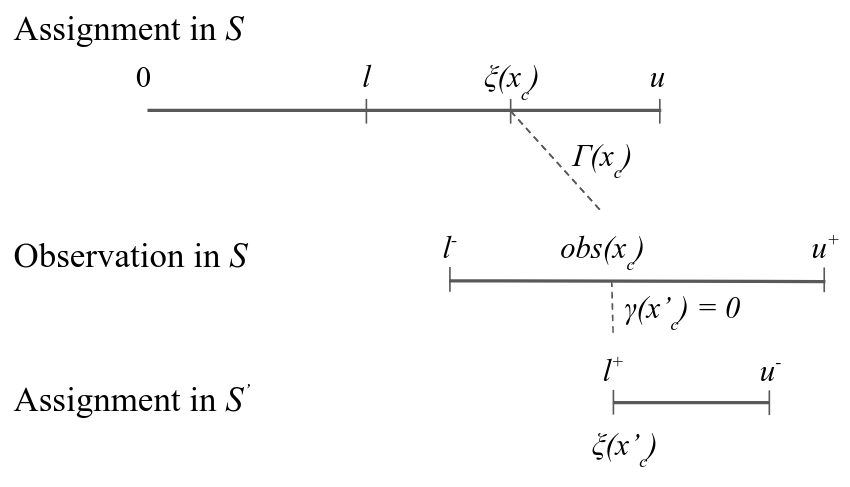
\includegraphics[width=3.5in]{images/viz-eqn-obs-assign.png}
\caption{\label{fig:obs-assign}We visualize the relationship between realized assignments across \(S\) and \(S'\). In this example, each horizontal line is a timeline monotonically increasing from left to right. Dashed lines represent observation delays. We see how an assignment in \(S\), \(\assign(x_{c})\), realized observation delay, \(\Gamma(x_{c})\), and an observation in \(S\), \(\obs(x_{c})\), contribute to an assignment in \(S'\), \(\assign(x'_{c})\).}
\end{figure}

Note that we receive \(\obs(x_{c})\) from Nature, but make the assignment \(\xi(x'_{c})\) in the
dispatchable form of \(S'\). To be clear, while \(\assign(x_{c})\) is an interval, \((\mathbb{R} \cup
\infty) \times (\mathbb{R} \cup \infty)\), \(\assign(x'_{c})\) is in \(\mathbb{R}\). For a fixed
interval, e.g. \(\obs(x_{c}) \in [t, t]\), we sometimes employ an equivalent representation,
\(\assign(x_{c}) = t\).


Additionally, we sometimes apply \(-\) and \(+\) superscripts to \(l\) and \(u\) to denote the earliest and
latest times respectively that an assignment at those bounds could be observed. For instance, the
relationship in Definition \ref{defn:vdc-obs} simplifies to,

\begin{align}
\label{eqn:obs-assign}
\label{eqn:obs-assign}
\obs(x_{c}) &= [l + \gammabar^-(x_{c}), u + \gammabar^+(x_{c})] \\
\obs(x_{c}) &= [l^-(x_{c}), u^+(x_{c})]
\end{align}

Lastly, we need a means to compare observation spaces if we are to transform variable-delay to
fixed-delay STNUs.

\begin{defn}
\textbf{Observation Space Mapping}

Let \(\mu\) be a mapping from an assignment to a situation, \(\mu : \xi \rightarrow \omega\). To say
that \(\mu(x'_{c}) \subseteq \omega_{v}(x_{c})\) means that, for any assignment of \(x'_{c}\) in \(S'\),
there is an equivalent situation in \(S\) for \(x_{c}\).
\end{defn}

For the transitions below, it is a \emph{valid observation space mapping}, if we can show that
\(\mu(x'_{c}) \subseteq \omega_{v}(x_{c})\). If so, it is guaranteed that any assignment in the
observation space of \(x'_{c}\) also has a valid assignment in the observation space of \(x_{c}\).

We now have the necessary vocabulary and notation to step through the transformations from \(S\) to
\(S'\). These lemmas were first presented in \citeprocitem{13}{[13]}, with some refinement by us for the
aforementioned journal article submission.

\begin{defn}
\textbf{Variable-Delay to Fixed-Delay Transformations}

The \emph{variable-delay to fixed-delay transformations} define a set of observation space mappings,
where there are valid observation space mappings for all the contingent constraints in \(S'\) to \(S\).
\end{defn}

Thus, if there is a satisfying \(\mathcal{S}\) for the fixed-delay observation space of \(S'\), it is guaranteed to
simultaneously satisfy any situation in the variable-delay observation space, \(\Omega_{v}\), of \(S\).

\begin{lemma}
\label{lemma:emulating-fixed}
For any contingent event \(x_c \in X_c\) in \(S\), if \(\gammabar^-(x_c) = \gammabar^+(x_c)\), we emulate
\(\gammabar(x_c)\) in \(S'\) using \(\gamma(x'_c) = \gammabar^+(x_c)\).
\end{lemma}

\begin{proof}
We translate an already fixed-bounded observation delay in the form of \(\gammabar(x_{c})\) to the
equivalent fixed-delay function, \(\gamma(x'_{c})\), thus \(\omega_{f}(x'_{c}) = \omega_{v}(x_{c})\).
\end{proof}

\begin{lemma}
\label{lemma:partially-unobservable}
For any contingent event \(x_c \in X_c\), \(\gammabar^+(x_c) = \infty\), we emulate \(\gammabar(x_c)\) in
\(S'\) as \(\gamma(x'_c) = \infty\).
\end{lemma}

\begin{proof}
There are projections where we would not receive information about \(x_{c}\), therefore we have to act
as if we \emph{never} receive an observation of \(x_{c}\). Any \(\mathcal{S}\) that works when we do not
receive information about \(x_{c}\) would also work when do receive an observation if we choose to
ignore the observation.

None of our decisions depend on \(\xi(x'_{c})\), thus no observation space mapping to \(S\) is
necessary.
\end{proof}

\begin{figure}[htbp]
\centering
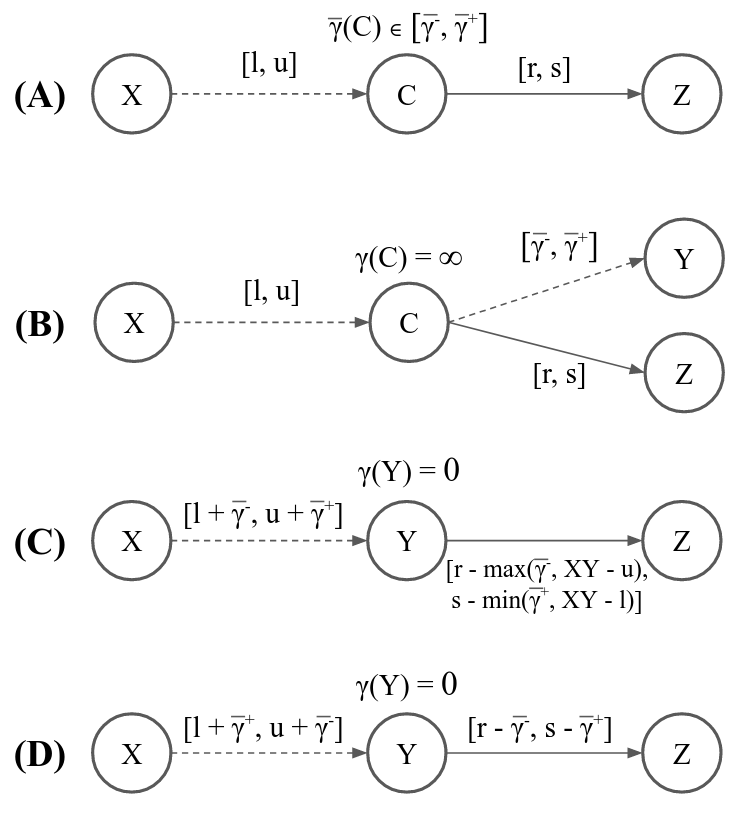
\includegraphics[width=.9\linewidth]{images/lemmas-combined.png}
\caption{\label{fig:lemmas-combined}A visualization of the lemmas used to transform contingent links with variable observation delay and subsequent requirement links.}
\end{figure}

\begin{lemma}
\label{lemma:not-enough-information}
If \(u - l \leq \gammabar^+(x_c) - \gammabar^-(x_c)\), we emulate \(\gammabar(x_c)\) in \(S'\) using
\(\gamma(x'_c) = \infty\).
\end{lemma}

\begin{proof}
We can ignore observations of \(x_{c}\) because they are not guaranteed to narrow where \(\assign(x_c)\)
was assigned in the range \([l, u]\).

Let \(\alpha\) be the range of \(\obs(x_{c})\) when \(\assign(x_{c}) \in [l, l]\). Let \(\beta\) be the
range of \(\obs(x_{c})\) when \(\assign(x_{c}) \in [u, u]\). By Equation \ref{eqn:obs-assign},

\begin{align*}
\alpha &= [l^-(x_{c}), l^+(x_{c})] \\
\beta &= [u^-(x_{c}), u^+(x_{c})]
\end{align*}

We can show that \(u^-(x_{c}) \leq l^+(x_{c})\).

\begin{align*}
u - l &\leq \gammabar^+(x_c) - \gammabar^-(x_{c}) \\
u + \gammabar^-(x_{c}) &\leq l + \gammabar^+(x_{c}) \\
u^-(x_{c}) &\leq l^+(x_{c})
\end{align*}

The lower bound of \(\beta\) is less than the upper bound of \(\alpha\), thus \(\alpha \cap \beta\). An
observation \(\obs(x_{c}) \in [u^-(x_{c}), l^+(x_{c})]\) could be the result of \(\assign(x_{c}) = [l,
l]\), \(\assign(x_{c}) = [u, u]\), or any value \(\assign(x_{c}) \in [l, u]\). Observations provide no
information about the underlying contingent constraint, therefore we ignore \(\obs(x_{c})\).

None of our decisions depend on \(\xi(x'_{c})\), thus no observation space mapping to \(S\) is
necessary.
\end{proof}

\begin{lemma}
\label{lemma:main-tightening}
If \(u - l > \gammabar^+(x_c) - \gammabar^-(x_c)\), we can emulate \(\gammabar(x_c)\) under minimal
information by replacing the bounds of \(x_c\) with \(x'_{c} \in [l^+(x_{c}), u^-(x_{c})]\) and letting
\(\gamma(x'_c) = 0\).
\end{lemma}

\begin{proof}
Under Lemma \ref{lemma:main-tightening}, observations \(\obs(x_{c})\) are guaranteed to narrow the range of
\(\assign(x_{c})\).

We have the same ranges for \(\alpha\) and \(\beta\) as in Lemma \ref{lemma:not-enough-information}, however
we can show that \(u^-(x_{c}) \geq l^+(x_{c})\) instead.

\begin{align*}
u - l &\geq \gammabar^+(x_c) - \gammabar^-(x_{c}) \\
u + \gammabar^-(x_{c}) &\geq l + \gammabar^+(x_{c}) \\
u^-(x_{c}) &\geq l^+(x_{c})
\end{align*}

Thus, receiving an observation is guaranteed to narrow the derived range of \(\assign(x_{c})\). The
transformation tightens the range of \(x'_{c}\) to one where there is maximum ambiguity of the
assignment of \(x_{c}\) while guaranteeing an execution strategy for any assignment of \(x_{c} \in [l,
u]\).
\end{proof}

After applying Lemma \ref{lemma:main-tightening}, despite the limited expected range of assignments in
\(x'_{c}\) in \(S'\) compared to \(x_{c}\) in \(S\), we can show that Lemma \ref{lemma:applied-execution}
guarantees a satisfying schedule for any \(\obs(x_{c}) \in [l^-(x_{c}), u^+(x_{c})]\) using an
\(\mathcal{S}\) that employs \emph{buffering} and \emph{imagining} contingent events.

\begin{defn}
\textbf{Buffering}

\emph{Buffering} a contingent event \(x_{c}\) is an execution strategy where, if \(x_{c}\) is observed
earlier than the lower bound of the observation space \(\obs(x_{c}) < \omega_{f}^-(x'_{c})\), we
assign \(\xi(x'_{c})\) to the lower bound of the observation space, \(\xi(x'_{c}) =
\omega_{f}^-(x'_{c})\).
\end{defn}

\begin{defn}
\textbf{Imagining}

\emph{Imagining} a contingent event \(x_{c}\) is an execution strategy where, if \(x_{c}\) is observed later
than the upper bound of the observation space, \(\obs(x_{c}) > \omega_{f}^+(x'_{c})\), we assign
\(\xi(x'_{c})\) to the upper bound of the observation space, \(\xi(x'_{c}) = \omega_{f}^+(x'_{c})\).
\end{defn}

\begin{lemma}
\label{lemma:buffering-imagining}
If \(S'\) is fixed-delay controllable after applying Lemmas \ref{lemma:main-tightening}, \ref{lemma:execution},
and \ref{lemma:applied-execution} to contingent event \(Y\) with following requirement event \(Z\), there is a
valid \(\mathcal{S}\) for any observation in the observation space of \(S\), \(\omega_{v}(Y) = [a^-(Y),
b^+(Y)]\).
\end{lemma}

\begin{proof}
We first note the observation space of \(S'\) is a subinterval of the original observation space of
\(S\), \(\omega_{f}(Y') \subset \omega_{v}(Y)\), and there are two distinct ranges of observations that
are not in \(\omega_{f}(Y')\).

\begin{align*}
\omega_{f}(Y') &= [a + \gammabar^+(Y), b + \gammabar^-(Y)];~\omega_{v}(Y) = [a + \gammabar^-(Y), b + \gammabar^+(Y)] \\
\omega_{f}(Y') &\not\supset [a + \gammabar^-(Y), a + \gammabar^+(Y))~~(\textit{"Early" observations}) \\
\omega_{f}(Y') &\not\supset (b + \gammabar^+(Y), b + \gammabar^+(Y)]~~(\textit{"Late" observations})
\end{align*}

We address the early observations first. The range of early assignments of \(\xi(Y)\) in \(S\) that we
care about are the ones that could produce an observation \(\obs(Y) \leq a + \gammabar^+(Y)\), which
is \(\xi(Y) = [a, a + (\gammabar^+(Y) - \gammabar^-(Y))]\). We rewrite the range of early assignments
as \(\xi(Y) = a + (\gammabar^+(Y) - \gammabar^-(Y)) - \epsilon\), where \(0 \leq \epsilon \leq
(\gammabar^+(Y) - \gammabar^-(Y))\). By the semantics of \(S\), the range of assignments of \(\xi(Z)\) is
then,

\begin{align*}
\xi(Z) &= [a + (\gammabar^+(Y) - \gammabar^-(Y)) - \epsilon, a + (\gammabar^+(Y) - \gammabar^-(Y)) - \epsilon] + [u, v] \\
\xi(Z) &= [a + u + (\gammabar^+(Y) - \gammabar^-(Y)) - \epsilon, a + v + (\gammabar^+(Y) - \gammabar^-(Y)) - \epsilon]
\end{align*}

The earliest assignment of \(Y'\) in \(S'\) is \(\xi(Y') = a + \gammabar^+(Y)\). By the semantics of \(S'\),
the range of assignments of \(\xi(Z')\) is then,

\begin{align*}
\xi(Z') &= [a + \gammabar^+(Y), a + \gammabar^+(Y)] + [u - \gammabar^-(Y), v - \gammabar^+(Y)] \\
\xi(Z') &= [a + u + (\gammabar^+(Y) - \gammabar^-(Y)), a + v]
\end{align*}

We see that \(\xi(Z') \subseteq \xi(Z)\) for any \(\epsilon\), meaning the execution strategy when
\(\xi(Y') = a + \gammabar^+(Y)\) results in a valid assignment of \(\xi(Z)\) for all early observations
of \(\xi(Y)\). We are safe to buffer early observations to \(\xi(Y') = a + \gammabar^+(Y)\).

We use the same argument for imagining late observations. The range of late assignments of \(\xi(Y)\)
in \(S\) that we care about are the ones that could produce an observation \(\obs(Y) \geq b +
\gammabar^-(Y)\), which is \(\xi(Y) = b - (\gammabar^+(Y) - \gammabar^-(Y)) + \epsilon\). By the
semantics of \(S\), the range of assignments of \(\xi(Z)\) is then,

\begin{align*}
\xi(Z) &= [b - (\gammabar^+(Y) - \gammabar^-(Y)) + \epsilon, b - (\gammabar^+(Y) - \gammabar^-(Y)) + \epsilon] + [u, v] \\
\xi(Z) &= [b + u - (\gammabar^+(Y) - \gammabar^-(Y)) + \epsilon, b + v - (\gammabar^+(Y) - \gammabar^-(Y)) + \epsilon]
\end{align*}

The last assignment of \(Y'\) in \(S'\) is \(\xi(Y') = b + \gammabar^-(Y)\). By the semantics of \(S'\),
the range of assignments of \(\xi(Z')\) is then,

\begin{align*}
\xi(Z') &= [b + \gammabar^-(Y), b + \gammabar^+(Y)] + [u - \gammabar^-(Y), v - \gammabar^+(Y)] \\
\xi(Z') &= [b + u, b + v - (\gammabar^+(Y) - \gammabar^-(Y))]
\end{align*}

We see that \(\xi(Z') \subseteq \xi(Z)\) for any \(\epsilon\), meaning the execution strategy when
\(\xi(Y') = b + \gammabar^-(Y)\) results in a valid assignment of \(\xi(Z)\) for all late observations
of \(\xi(Y)\). In practice, there is no reason to wait until after \(\obs(Y) = b + \gammabar^-(Y)\) to
receive a late observation. As soon as we see the clock has reached \(b + \gammabar^-(Y)\), we are
safe to imagine that \(\obs(Y)\) has been received.
\end{proof}

This concludes the modifications required to transform a contingent event \(x_{c} \in X_{c}\) in \(S\)
to its equivalent \(x'_{c} \in X_{c}\) in \(S'\). What remains is to address the transformation of
requirement links, \(x_{r} \in X_{r}\), in \(S\) such that their transformed equivalents, \(x'_{r} \in
X_{r}\) in \(S'\), express the same execution semantics in \(S'\) as they did in \(S\). We will demonstrate
the correctness of the transformations after Lemma \ref{lemma:applied-execution}.

\begin{lemma}
\label{lemma:execution}
If we have contingent link \(\conedge{X}{C}{}\) with duration \([l, u]\), outgoing requirement link
\(\edge{C}{Z}{}\) with duration \([u, v]\) with an unobservable \(C\), and contingent link
\(\conedge{C}{Y}{}\) with range \([\gammabar^-(x_{c}), \gammabar^+(x_{c})]\), we can emulate the role of
the original requirement link during execution with a new link \(\edge{Y}{Z}{}\) with bounds \([u -
max(\gammabar^-(x_{c}), XY - u), v - min(\gammabar^+(x_{c}), XY - l)]\), where \(XY\) is the true
duration of \(\conedge{X}{Y}{}\).
\end{lemma}

\begin{proof}
See Figure \ref{fig:lemmas-combined}c for reference. From an execution perspective, \(X\) and \(Y\) are
the only events that can give us any information that we can use to reason about when to execute \(Z\)
(since \(C\) is wholly unobservable).

If we execute \(Z\) based on what we learn from \(Y\), then we use our information from \(Y\) to make
inferences about the true durations of \(\conedge{X}{C}{}\) and \(\conedge{C}{Y}{}\) based on
\(\conedge{X}{Y}{}\). We know that the lower-bound of \(\conedge{C}{Y}{}\) is at least \(XY - b\) and that
its upper-bound is at most \(XY - a\). But we also have the a priori bounds on the contingent link
that limit its range to \([\gammabar^-, \gammabar^+]\). Taken together, during execution we can infer
that the true bounds of \(\conedge{C}{Y}{}\) are \([max(\gammabar^-, XY - b), min(\gammabar^+, XY -
a)]\). Since we have bounds only on \(Z\)'s execution in relation to \(C\), we can then infer a
requirement link \(\edge{Y}{Z}{}\) with bounds \([u - max(\gammabar^-, XY - b), v - min(\gammabar^-,
XY - a)]\).

If we try to execute \(Z\) based on information we have about \(X\), we must be robust to any possible
value assigned to \(\conedge{X}{C}{}\). This means that we would be forced to draw a requirement link
\(\edge{X}{Z}{}\) with bounds \([u+b, v+a]\). But we know that \(u - max(\gammabar^-, XY - b) \leq u +
b - XY\) and \(v - min(\gammabar^-, XY - a) \geq v + a - XY\), which means that the bounds we derived
from \(Y\) are at least as expressive as the bounds that we would derive from \(X\).
\end{proof}

Since we have a local execution strategy that depends on the real value of \(XY\), we can try to apply
this strategy to the contingent link that we restricted in Lemma \ref{lemma:main-tightening}, in
order to repair the remaining requirement links.

\begin{lemma}
\label{lemma:applied-execution}
If we have an outgoing requirement link \(\edge{C}{Z}{}\) with duration \([u, v]\), where \(C\) is a
contingent event, we can emulate the role of the original requirement link by replacing its bounds
with \([u - \gammabar^-(x_{c}), v - \gammabar^+(x_{c})]\).
\end{lemma}

\begin{proof}
See Figure \ref{fig:lemmas-combined}d for reference. If we directly apply the transformation from Lemma
\ref{lemma:execution} and Figure \ref{fig:lemmas-combined}c to our original STNU, we introduce complexity
through the need to reason over \(min\) and \(max\) operations in our link bounds. However, from Lemma
\ref{lemma:main-tightening}, we know that in a controllability evaluation context, it is acceptable
for us to simplify the \(\conedge{X}{Y}{}\) link to a stricter range of \([a + \gammabar^+, b +
\gammabar^-]\), instead of \([a + \gammabar^-, b + \gammabar^+]\). This means that for the purpose of
evaluating controllability, we can assume \(a + \gammabar^+ \leq XY \leq b + \gammabar^-\). When we
evaluate the requirement link \(\edge{Y}{Z}{}\), we see \(max(\gammabar^-, XY - b) = \gammabar^-\) and
\(min(\gammabar^+, XY - a) = \gammabar^+\). This gives us bounds of \([u - \gammabar^-, v -
\gammabar^+]\) for the \(\edge{Y}{Z}{}\) requirement link as seen in Figure \ref{fig:lemmas-combined}d.
\end{proof}

Lemma \ref{lemma:applied-execution} handles outgoing requirement edges connected to contingent
events. In addition, we must handle incoming edges.

\begin{corollary}
\label{corollary:reversed}
If we have an incoming requirement link \(\edge{Z}{C}{}\) with duration \([u, v]\), where \(C\) is a
contingent event, we can replace the bounds of the original requirement link with \([u +
\gammabar^+(x_{c}), v + \gammabar^-(x_{c})]\).
\end{corollary}

\begin{proof}
A requirement link \(\edge{Z}{C}{}\) with bounds \([u, v]\) can be immediately rewritten as its reverse
\(\edge{C}{Z}{}\) with bounds \([-v, -u]\). After reversing the edge, we can apply Lemma
\ref{lemma:applied-execution} to get \(\edge{Y}{Z}{}\) with bounds \([-v - \gammabar^-, -u -
\gammabar^+]\), which we can reverse again to get \(\edge{Z}{Y}{}\) with bounds \([u + \gammabar^+, v +
\gammabar^-]\).
\end{proof}

We can examine a concrete example of Lemmas \ref{lemma:main-tightening}, \ref{lemma:execution}, and
\ref{lemma:applied-execution} to show equivalence in the transformation from Figure \ref{fig:lemmas-combined}a
to \ref{fig:lemmas-combined}d. We start by building an example of \ref{fig:lemmas-combined}a. Let
\(\conedge{X}{C}{[2, 5]}\) with \(\gammabar(C) \in [1, 2]\) and \(\edge{C}{Z}{[11, 20]}\). If we learn of
event \(C\) at time 4, then one possibility is that the realized duration of \(C\) could have been 2
with an observation delay of 2. In this case, event \(Z\) must be executed in \([13, 22]\). However, if
the realized duration of \(C\) were 3 with an observation delay of 1, then \(Z\) would fall in \([14,
23]\). Given we cannot distinguish between the possibilities, we take the intersection of the
intervals, yielding \(Z \in [14, 22]\). Likewise, if we learn of \(C\) at time 6, then \(C\) could have
been realized at time 5 with an observation delay of 1 or it could have been realized at time 4 with
an observation delay of 2. In the first case, \(Z\) must then fall in \([16, 25]\), while in the second,
\(Z\) would fall in \([15, 24]\). The intersection yields \([16, 24]\).

By the semantics represented in Figure \ref{fig:lemmas-combined}d, we can build an equivalent network with
\(\gamma(Y) = 0\) by setting \(\conedge{X}{Y}{[4, 6]}\) and \(\edge{Y}{Z}{[10, 18]}\). If \(Y\) is observed
at time 4, \(Z\) must be executed in \([14, 22]\). If \(Y\) is observed at time 6, \(Z\) then must be
executed in \([16, 24]\). The execution semantics for both cases match the equivalent networks from
\ref{fig:lemmas-combined}a described above.

\section{Discussion}
\label{sec:orga86a108}

We have demonstrated a modeling formalism to describe temporal networks with uncertain observation
delay, along with a sound and complete procedure for checking controllability of said temporal
networks. VDC is sound because if it finds that \(S'\) has a valid execution strategy, then it must
also be the case that \(S\) has an execution strategy. VDC is complete because if it finds that \(S'\)
is not controllable, then there exists a projection of \(S\) that is uncontrollable, thus \(S\) is not
variable-delay controllable.

\section{Experimental Analysis}
\label{sec:org792b880}
\label{sec:vdc-experimental}

In this section, we provide empirical evaluations of our variable-delay controllability checking
algorithms, showing that variable-delay controllability gives us a level of modeling expressiveness
that cannot be captured by approximations that use delay controllability alone. We do so by
constructing examples of variable-delay STNUs for realistic multi-agent coordination scenarios that
are taken from the domain of planetary exploration, inspired by the real decision-making processes
during Apollo EVAs and modern day EVA operations research. First, we briefly describe the
operational environment, relevant actors, and decisions in EVAs. We then provide a selection of
STNUs that reflect the activities and temporal constraints of planetary exploration. Using these
building blocks, we make a case for the expressivity of VDC in modeling uncertain communication,
then generate larger STNUs to demonstrate the soundness of variable-delay controllability
checking.\footnote{The implementation of the experiments herein can be found at
\href{https://gitlab.com/mit-mers/delay-stnu-benchmarks}{[https://gitlab.com/mit-mers/delay-stnu-benchmarks}].}

\begin{figure}[htbp]
\centering
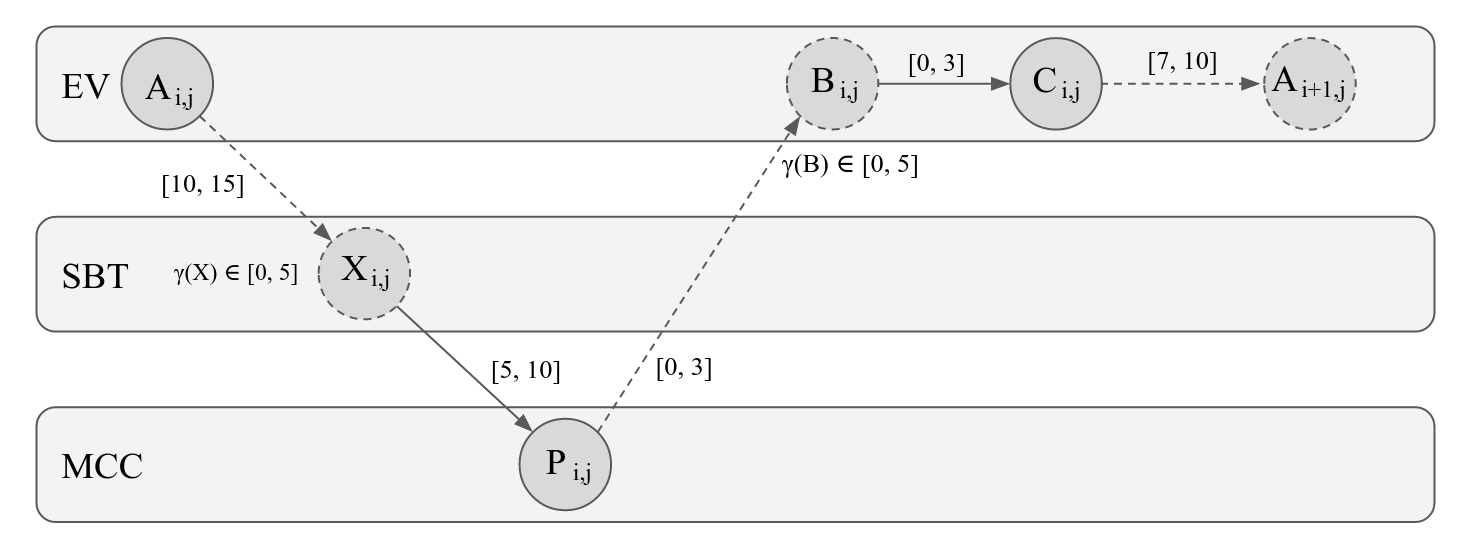
\includegraphics[width=1\textwidth]{images/eva-stnu.png}
\caption{\label{fig:sbt-stnu}An STNU representing an EVA sampling task. The episode durations are representative of the bounds used in simulation. The depiction of this STNU with variable-delay is presented with rows representing actors to clarify the context of each event.}
\end{figure}

Now, we present a sample collection communication scenario in Figure \ref{fig:sbt-stnu} that is
representative of the types of activities performed during exploration and requires uncertain
communication delay to faithfully model.

At a high level, in this activity a crew of \(i\) astronauts perform \(j\) activities of scanning
potential samples and receiving feedback from the science team as to whether they should store or
discard those sample. Scanning requires liberating, that is chipping away, a piece of rock from an
outcrop, \(A_{i,j}\), and performing a scan of the newly exposed surface with a handheld spectrometer.
Spectroscopy data is eventually received at \(X_{i,j}\); we model this duration of this process with
the contingent link \(\conedge{A_{i,j}}{X_{i,j}}{}\) where \(X_{i,j}\) is uncontrollable because the
time to liberate and scan is a function of the environment (eg. how hard the sample is to access),
not the crew. The processing completion time of the handheld spectrometer is highly variable, and as
such we have \(\gammabar({X_{i,j}})\) represent a variable delay in receiving the results of the scan.
Interestingly, note that the general time of \(A_{i,j}\) will be known immediately through the use of
audio and video communications - the variability of \(X_{i,j}\) refers to the delay of receiving the
spectroscopy data itself.

During a narrow window of opportunity between the receipt of the sample information and a deadline
imposed by Mission Control, \(P_{i,j}\), the science team must confer and decide on a sample
collection priority list to send to Mission Control, \(\edge{X_{i,j}}{P_{i,j}}{}\). Even once Mission
Control has a sample priority list in hand, \(P_{i,j}\), due to health and safety concerns, they may
prioritize other messages before they send the science team's sampling priority decision to the
crew. As such, the message passing process, \(\conedge{P_{i,j}}{B_{i,j}}{}\), is modeled as
uncontrolled with a variable communication delay. Once the crew receives the priority list, \(B\),
they then stow the requested amount of samples at \(C_{i,j}\). Then the astronaut traverses to the
next location and the procedure repeats anew. We use \(\conedge{C_{i,j}}{A_{i,j+1}}{}\) to model the
time needed to traverse to the site of the next activity. We apply a requirement link with a
lower-bound of 0 and an upper bound of the limiting consumable from the overall start of each STNU
to its overall end after each astronaut has completed all activities.

With realistic STNUs in hand, we can now evaluate the performance of our variable-delay
formulations. For the simulations presented in subsequent sections, we generated STNUs that follow
the form of Figure \ref{fig:sbt-stnu} with randomized bounds on the links and delay functions, as will be
described below.

\begin{table*}[t]
\centering
\begin{tabular}{ |>{\centering\arraybackslash} m{4.4cm}||>{\centering\arraybackslash} m{4.5cm}|>{\centering\arraybackslash} m{5.0cm}|  }
 \hline
 & Variable-delay controllable & Variable-delay uncontrollable\\
 \hline
 \hline
 Min-fixed controllable & 222 & 619\\
 \hline
 Min-fixed uncontrollable & 0 & 159\\
 \hline
 \hline
 Mean-fixed controllable & 222 & 583\\
 \hline
 Mean-fixed uncontrollable & 0 & 195\\
 \hline
 \hline
 Max-fixed controllable & 222 & 355\\
 \hline
 Max-fixed uncontrollable & 0 & 423\\
 \hline
\end{tabular}
\caption{Variable-delay vs. minimum, mean, and maximum fixed-delay controllability results with the parallel installation STNU from Figure \ref{fig:dish-stnu}.}
\label{table:comparison}
\end{table*}

We now will evaluate the comparative quality of variable-delay formulations against fixed-delay
approximations by using the repeater installation scenario seen in Figure \ref{fig:dish-stnu}. We
generate STNUs with four astronauts each performing five installations. We set the lower bounds of
\(\conedge{A_{i,j}}{B_{i,j}}{}\) to 0 and choose the upper bounds from a uniform distribution of
integers between 0 and 20, \(\mathcal{U}_{[0, 20]}\). There is no delay function for \(B_{i,j}\).
Likewise, for \(\edge{B_{i,j}}{C_{i,j}}{}\), we set the lower bounds to 0 and choose an integer upper
bound in \(\mathcal{U}_{[0, 15]}\). \(\conedge{C_{i,j}}{D_{i,j}}{}\) has a lower bound of 0 and an upper
bound integer chosen in \(\mathcal{U}_{[0, 20]}\). The variable-delay function \(\gamma(D_{i,j})\) has a
lower bound of 0 and upper-bound chosen from the exponential distribution \(f(t) = \lambda
e^{-\lambda t}\) with \(\lambda = 3\). \(\conedge{D_{i,j}}{A_{i,j+1}}{}\) takes a lower bound integer,
\(a\), from \(\mathcal{U}_{[10, 20]}\) and its upper bound in \(a + \mathcal{U}_{[4, 10]}\). Lastly, we
pick a random limiting consumable as the multiple of the number of activities and an integer from
\(\mathcal{U}_{[50, 60]}\).

We employ three different strategies for each \(\gamma(x_c)\) in \(S\) for our fixed-delay
approximations: \(\gamma(x_c) = \gammabar^-(x_c)\), \(\gamma(x_c) = \frac{\gammabar^- +
\gammabar^+}{2}\), and \(\gamma(x_c) = \gammabar^+(x_c)\). For each strategy, we know that whenever the
original STNU is variable-delay controllable with respect to \(\gammabar\), it is also fixed-delay
controllable with respect to \(\gamma\). Each choice of \(\gamma\) represents a potential realization of
the delays offered by \(\gammabar\), and the fixed-delay approximation has the added benefit of
eliminating uncertainty in observation.

We generate 1000 different STNUs and compare the variable-delay controllability results to the
different fixed-delay controllability approaches (Table \ref{table:comparison}). Note that our randomly
generated variables, notably the choice of \(\gamma(C_{i,j})\) and the width of the following
\(\edge{C_{i,j}}{D_{i,j}}{}\) link, were selected such that the STNUs generated could be
variable-delay, fixed-delay, dynamic, or strong controllable, or uncontrollable. The instances that
are of greatest interest are those where the STNU is not variable-delay controllable but the
fixed-delay approximations determine it to be controllable.

This false positive rate of the minimum fixed-delay controllability approximation is quite high at
80.0\%. The mean and maximum fixed-delay approximations have more reasonable false positive rates at
74.9\% and 45.6\% respectively. Since all approximations yield the correct answer when the original
STNU is variable-delay controllable, it follows that the maximum fixed-delay approximation has the
lowest false positive rate, as it is the most demanding of the three.

We note that these results are dependent on the width of the variable-delay ranges found in the
network. We can increase the likelihood that a delay takes longer by increasing the choice of
\(\lambda\) in our exponential delay function. When we vary our delay function using \(\lambda = 4.5,
6, 7.5\), and \(9\), the false positives of the max-delay approximation are 27.9\% 12.9\%, 7.0\%, and
3.1\%, respectively.

In addition to simulating the network using fixed-delays, we also consider the effect of combining
the two sources of uncertainty, the duration of the action and the delay in observation, into one
new source of uncertainty. Unlike the fixed-delay approximations, we know that if a network under
this transformation is controllable, then so too is the original network, as this approach discards
any existing knowledge about the difference in uncertainties between the original event and the
observation of that event.

\begin{table*}[t]
\centering
\begin{tabular}{ |>{\centering\arraybackslash} m{4.4cm}||>{\centering\arraybackslash} m{4.5cm}|>{\centering\arraybackslash} m{5.0cm}|  }
 \hline
 & Variable-delay controllable & Variable-delay uncontrollable\\
 \hline
 \hline
 Elongated controllable & 36 & 0\\
 \hline
 Elongated uncontrollable & 186 & 778\\
 \hline

\end{tabular}
\caption{Variable-delay controllability vs. the controllability of a network that elongates its contingent links to account for observational uncertainty when using an exponential delay function with $\lambda = 3$.}
\label{table:comparison-elongated}
\end{table*}

As seen in Table \ref{table:comparison-elongated}, this approach yields no false positives, but still
presents a modestly high false negative rate of 19.3\%. An appropriate approximation strategy can be
adopted to prevent either false positives or false negatives; however, such a wide disparity in
results strongly reinforces the value of modeling observational uncertainty directly.

\chapter{Scheduling Events Despite Uncertain Observations}
\label{sec:orgd2c935d}
\label{ch:delay-scheduling}

Now that we have shown there exists a valid execution strategy for variable-delay controllable
STNUs, we contribute a novel scheduling and dispatching architecture for online, dynamic execution.
In this Chapter, our aim is to describe the single-agent form of a new instantiation of Kirk, \emph{Delay
Kirk}, that can reason over uncertain observation delay to decide when to execute requirement events
on real hardware. There are two main components to Delay Kirk: (1) a \emph{delay scheduler}, and (2) a
\emph{delay dispatcher}. As will be shown in Section \ref{sec:delay-scheduling}, scheduling variable-delay
controllable STNUs is an extension to existing dynamic scheduling algorithms with modifications for
the execution strategy shown to be sound and complete in Chapter \ref{ch:modeling-tn}.

Additionally, to the best of our knowledge, scheduling fixed-delay STNUs has not been presented in
the literature. Fixed-delay scheduling is required for addressing (1). As such, we contribute a
fixed-delay scheduler in Section \ref{sec:delay-scheduling}. The execution strategy from Chapter
\ref{ch:modeling-tn} will be shown to be a small extension to the fixed-delay scheduler. As to (2), to the
best of our knowledge, there are no other formalized dispatching algorithms in the literature. In
the development of Delay Kirk, we found it to be extremely useful to formalize dispatching as part
of creating a clear interface boundary between scheduling and dispatching. The dispatching
algorithms we put forth in Section \ref{sec:dynamic-dispatching} represent novel contributions to temporal
reasoning.

This Chapter makes additional contributions to scheduling and dispatching. Safely executing events
on real hardware requires modifications to generating decisions in dynamic scheduling. We include
said modifications, with confluent interfaces in dynamic dispatching, to suit our intended use cases
for Delay Kirk.

In Section \ref{sec:optimistic-rescheduling}, we extend our approach to scheduling variable-delay STNUs by
introducing an optional procedure that addresses a shortcoming in the semantics of scheduling a
variable-delay STNU. The shortcoming takes the form of potentially unnecessary wait times that are
added after receiving contingent event assignments, extending the makespan of procedures. We present
a generate-and-test algorithm to partially mitigate said shortcomings.

Finally, Section \ref{sec:scheduling-experimental} provides a series of benchmarks of the scheduling and
dispatching algorithms described in this Chapter.

\section{Dynamic Scheduling through Real-Time Execution Decisions}
\label{sec:org6d4fe4a}
\label{sec:dynamic-scheduling}

We first provide a necessary overview of dynamic scheduling of vanilla STNUs, which we will extend
for STNUs with observation delay in Section \ref{sec:delay-scheduling}.

An STNU, \(S\), that exhibits dynamic controllability can be \emph{scheduled} dynamically (or \emph{online}). At
a high-level, dynamic scheduling is the process of mapping the history of event assignments to the
execution time of future free events. We will build off of the scheduling work by Hunsberger
\citeprocitem{14}{[14]}, \citeprocitem{15}{[15]}, which describes an \(O(N^{3})\) online procedure, FAST-EX, for
dynamic scheduling of STNUs. We chose FAST-EX because, to the best of our knowledge, this is the
fastest dynamic scheduling algorithm in the literature today. At its core is the notion of
\emph{Real-Time Execution Decisions} (RTEDs), which map a time to a set of requirement events to be
executed and are generated based on \emph{partial schedules} of STNUs being executed. \texttt{WAIT} decisions
may also be produced, reflecting the need to wait for the assignment of a contingent event before
continuing. RTED-based scheduling applies a dynamic programming paradigm in three steps:

\begin{enumerate}
\item creating a dispatchable form of temporal constraints offline in the form of a distance graph,
\item updating the dispatchable form as the partial schedule is updated online through event
assignments, and
\item querying the dispatchable form online to quickly find the next RTED \citeprocitem{34}{[34]}.
\end{enumerate}

The dispatchable form employed by FAST-EX is the \emph{AllMax} distance graph, which is first described
in the Morris \(O(N^{4})\) DC-checking procedure \citeprocitem{31}{[31]}.

\begin{defn}
\textbf{AllMax Distance Graph} \citeprocitem{32}{[32]}

The \emph{AllMax} distance graph is a distance graph exclusively consisting of unlabeled and upper-case
edges.
\end{defn}

The key idea of FAST-EX is maintaining accurate distances from an artificial zero point, \(Z\), of the
distance graph to all events. At the outset of execution, all events from \(S\) are present as nodes
in \emph{AllMax}. As events are assigned, \emph{AllMax} performs update steps using Dijkstra Single
Source/Sink Shortest Path (SSSP) to maintain distances to unexecuted events, while also collapsing
executed events to \(Z\). We include pseudo-code of the real-time update step in Figure
\ref{alg:fast-ex-update}.

\begin{algorithm}
\SetAlgoLined
\SetKwFunction{Return}{return}
\SetKwInput{Input}{Input}
\SetKwInput{Output}{Output}
\SetKwInput{Algorithm}{\textsc{FAST-EX Update}}
\SetKwInput{Initialize}{Initialization}
\SetKwIF{If}{ElseIf}{Else}{if}{then}{else if}{else}{endif}
\Indm
\Input{Time $t$; Set of newly executed events $\texttt{Exec} \subseteq X_{e} \cup X_{r}$; AllMax Graph $G$; Distance matrix $D$, where $D(A, B)$ is the distance from $A$ to $B$}
\Output{Updated $D$}
\Indp
\Algorithm{}
\Indp
\For{each contingent event $C \in \texttt{Exec}$} {
    Remove each upper-case edge, $\edge{Y}{A}{C:-w}$, labled by $C$\;
    Replace each edge from $Y$ to $Z$ with the strongest replacement edge\;
}
\For{each event $E \in \texttt{Exec}$} {
    Add lower-bound edge $\edge{E}{Z}{-t}$\;
}
For each event $X$, update $D(X, Z)$ using Dijkstra Single-Sink Shortest Paths\;
\For{each event $E \in \texttt{Exec}$} {
    Add upper-bound edge $\edge{Z}{E}{t}$\;
}
For each event $X$, update $D(Z, X)$ using Dijkstra Single-Source Shortest Paths\;
\caption{Algorithm for updating distances for all events in relation to $Z$ upon the execution of an event. Adapated from \citeprocitem{3}{[3]}, Fig. 19.}
\label{alg:fast-ex-update}
\end{algorithm}

With an up-to-date distance graph in hand, we can perform an online query for the current RTED.

\begin{defn}
\textbf{Real-Time Execution Decisions} \citeprocitem{34}{[34]}

A \emph{Real-Time Execution Decision} is a two-tuple \(\langle t, \chi \rangle\), where:
\begin{itemize}
\item \(t\) is a time with domain \(\mathbb{R}\),
\item \(\chi\) is a set of \(x_{r} \in X_{r}\) to be executed at time \(t\)
\end{itemize}
\end{defn}

Let \(U_{x}\) be the set of unexecuted free timepoints. If \(U_{x}\) is empty, then the RTED is to
\texttt{WAIT}. Otherwise, we find the lower bound of the earliest executable time point and the set of
executable events associated with it.

\begin{align}
\label{eqn:rted1}
t &= \min\{-D(X, Z)~|~X \in U_{x}\} \\
\label{eqn:rted-chi}
\chi &= \{X \in U_{x}~|~-D(X, Z) = t\}
\end{align}

We cannot execute events in the past. Let \texttt{now} be the current time, i.e. the last timepoint
captured in the event assignments. It is possible that \(t \leq \texttt{now}\), in which case we must
reassign \(t\) to guarantee that \(t > \texttt{now}\). To do so, we update \(t\) as follows, where \(t^+\)
is earliest upper bound of the executable timepoints,

\begin{align}
\label{eqn:rted2}
t^+ &= \min\{D(Z, X)~|~X \in U_{x}\} \\
\label{eqn:rted-t}
t &= \cfrac{\texttt{now} + t^+}{2}
\end{align}

So long as \(t^+ > \texttt{now}\), we know that the reassignment of \(t\) ensures \(t > \texttt{now}\).

\section{Delay Scheduling as an Extension to Dynamic Scheduling}
\label{sec:orgb8b856c}
\label{sec:delay-scheduling}

\begin{figure}[htbp]
\centering
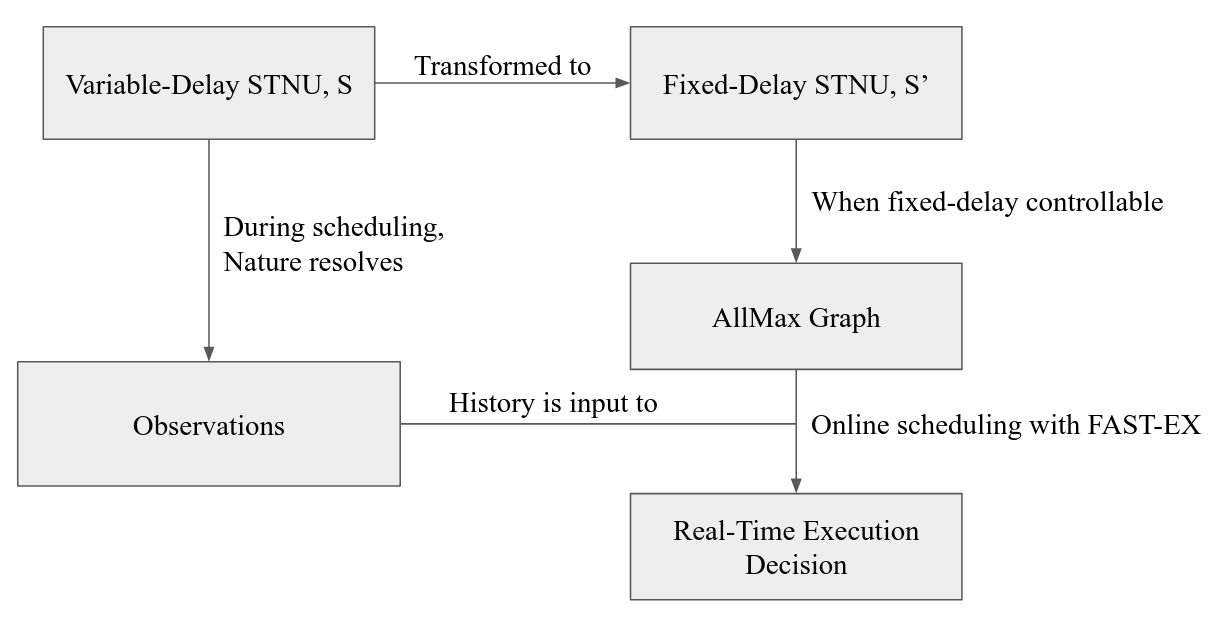
\includegraphics[width=0.8\textwidth]{images/flow-chart.png}
\caption{\label{fig:flow-chart}A high-level flow chart showing how we use variable-delay STNUs to generate scheduling decisions. The boxes represent the data structures involved in scheduling, while the arrows are the processes that are followed to eventually produce RTEDs.}
\end{figure}

Figure \ref{fig:flow-chart} presents a high-level overview of the information flow in the scheduling
process.

In order to schedule a variable-delay STNU, the core problem we must address is that, to date, there
is no means to directly create a corresponding dispatchable form that accounts for uncertain
assignments resulting from variable observation delay. We encountered this same problem when
describing the process of checking VDC in Section \ref{sec:vdc}. We overcame this limitation by first
transforming the variable-delay STNU to a fixed-delay STNU before checking FDC. A similar strategy
will be followed for scheduling in that we will transform the variable-delay to a fixed-delay STNU,
then dispatch events using the dispatchable form of the fixed-delay STNU instead. However, doing so
creates a second problem. While we will be performing FAST-EX against the fixed-delay STNU, the
contingent event observations we receive will adhere to the constraints and variable-delay function
of the variable-delay STNU. Hence, we must modify our real-time update and RTED generation
algorithms to account for early and late contingent event observations.

We start by providing an explanation of fixed-delay scheduling, before expanding it to address the
execution strategies of variable-delay scheduling.

\subsection{Fixed-Delay Scheduling}
\label{sec:orga82ac98}

We first establish the algebra of receiving observations.

\begin{lemma}
\label{lemma:information-fixes-bounds}
For any contingent event, \(x_{c} \in S\) or \(x'_{c} \in S'\), observing \(x_{c}\) at time \(t \in
[l^-(x_{c}), u^+(x_{c})]\) fixes the observation to \(\obs(x_{c}) = [t, t]\).
\end{lemma}
\begin{proof}

Prior to execution, an observation of \(x_{c}\) may fall anywhere within the set-bounded interval from
the earliest possible observation at \(l^-(x_{c})\) to the last possible observation at \(u^+(x_{c})\).
Receiving an observation \(\obs(x_{c}) = t\) during execution eliminates all possible observations
outside the interval \([t, t]\).
\end{proof}

\begin{lemma}
\label{equal-is-fixed-bounds}
For any temporal constraint, \(x\), with bounds \(x \in [l, u]\) for some \(l\) and \(u\), and timepoint \(t
\in [l, u]\), if information reduces the bounds of \(x\) to \(x \in [t, t]\), we may assert \(x = t\).
\end{lemma}

\begin{proof}

When the bounds of an interval, \(x \in [l, u]\) are fixed such that \(t = l = u\), we can assert that
\(x\) must have resolved to \(t\).
\end{proof}

\begin{lemma}
\label{lemma:subtract-gamma}
For any contingent event \(x'_{c} \in X_{c}\) in fixed-delay controllable \(S'\), if \(\gamma(x'_{c}) \in
\mathbb{R}\), we assign \(\assign(x'_{c}) = \obs(x_{c}) - \gamma(x'_{c})\) in the dispatchable form of
\(S'\).
\end{lemma}

\begin{proof}
The central challenge of checking fixed-delay controllability is determining that an execution
strategy exists that allows an agent to wait an additional \(\gamma(x'_{c})\) time units after a
contingent event has been assigned to learn its outcome. Importantly, the \(\gamma\) function is not
used to modify the edges of the labeled distance graph, which are derived from the constraints \(r
\in R_{e} \cup R_{c}\) in \(S'\).

As \(\gamma(x'_{c})\) resolves to a known and finite value, we can derive the true value of
\(\assign(x'_{c})\) to be assigned in the labeled distance graph. Contingent event assignments are
recorded in the labeled distance graph as follows, where \(\obs(x_{c})\) is the resolved observation,

\begin{align}\assign(x'_c) = \obs(x_c) - \gamma(x'_c) \label{eqn:fixed-recording}
\end{align}
\end{proof}

The FAST-EX real-time update algorithm, Algorithm \ref{alg:fast-ex-update}, then becomes Algorithm
\ref{alg:fast-ex-fixed-obs}.

\begin{algorithm}
\SetAlgoLined
\SetKwFunction{Return}{return}
\SetKwInput{Input}{Input}
\SetKwInput{Output}{Output}
\SetKwInput{Algorithm}{\textsc{FAST-EX Update with Fixed Observation Delay}}
\SetKwInput{Initialize}{Initialization}
\SetKwIF{If}{ElseIf}{Else}{if}{then}{else if}{else}{endif}
\Indm
\Input{Time $t$; Set of newly observed events $\texttt{Exec} \subseteq X_{e} \cup X_{r}$; AllMax Graph $G$; Distance matrix $D$, where $D(A, B)$ is the distance from $A$ to $B$; Fixed-delay function $\gamma$;}
\Output{Updated $D$}
\Indp
\Algorithm{}
\Indp
\For{each contingent event $C \in \texttt{Exec}$} {
    $\assign(C) \leftarrow \obs(C) - \gamma(C)$\;
    Remove each upper-case edge, $\edge{Y}{A}{C:-w}$, labled by $C$\;
    Replace each edge from $Y$ to $Z$ with the strongest replacement edge\;
}
\For{each event $E \in \texttt{Exec}$} {
    Add lower-bound edge $\edge{E}{Z}{-t}$\;
}
For each event $X$, update $D(X, Z)$ using Dijkstra Single-Sink Shortest Paths\;
\For{each event $E \in \texttt{Exec}$} {
    Add upper-bound edge $\edge{Z}{E}{t}$\;
}
For each event $X$, update $D(Z, X)$ using Dijkstra Single-Source Shortest Paths\;
\caption{Algorithm for updating distances for all events in relation to $Z$ upon the execution or observation of an event.}
\label{alg:fast-ex-fixed-obs}
\end{algorithm}

No other modifications to FAST-EX are required to schedule a fixed-delay STNU.

\subsection{Variable-Delay Scheduling}
\label{sec:org937d4ab}

Our execution strategy must address each of the following special categories of contingent event
observations:

\begin{enumerate}
\item contingent events with infinite observation delay,
\item contingent events that are observed outside \([l^+(x_{c}), u^-(x_{c})]\) in \(S'\).
\end{enumerate}

The first category is a requirement for dispatching the fixed-delay equivalent of a variable-delay
STNU. If the constraints of a problem domain are modeled directly in a fixed-delay STNU and the
modeler gives a contingent event, \(x_{c}\), infinite delay, e.g. \(\gamma(x_{c}) = \infty\), the event
will never be observed and thus a fixed-delay scheduler has no need for an execution strategy in the
event that \(x_{c}\) is observed. However, by Lemmas \ref{lemma:partially-unobservable} and
\ref{lemma:not-enough-information} there are some contingent events with potentially finite observation
delay in \(S\) that are transformed to infinite observation delay in \(S'\), making it possible that the
scheduler receives observations of them.

\begin{lemma}
\label{lemma:ignore-inf-delay}
For any contingent event \(x'_{c} \in X_{c}\) in fixed-delay controllable \(S'\), if \(\gamma(x'_{c}) =
\infty\), we mark the event executed but do not assign \(\assign(x'_{c})\) in the dispatchable form of
\(S'\).
\end{lemma}

\begin{proof}
If we are scheduling a fixed-delay STNU, \(S'\), that is already known to be fixed-delay controllable,
an execution strategy must exist that is independent of the assignment of \(\assign(x'_{c})\) when
\(\gamma(x'_{c}) = 0\). We are not required to record \(\assign(x'_{c})\) when \(\gamma(x'_{c}) = \infty\)
to guarantee controllability and may safely ignore it.

We mark the event executed to prevent it from appearing in future RTEDs.
\end{proof}

\begin{figure}[htbp]
\centering
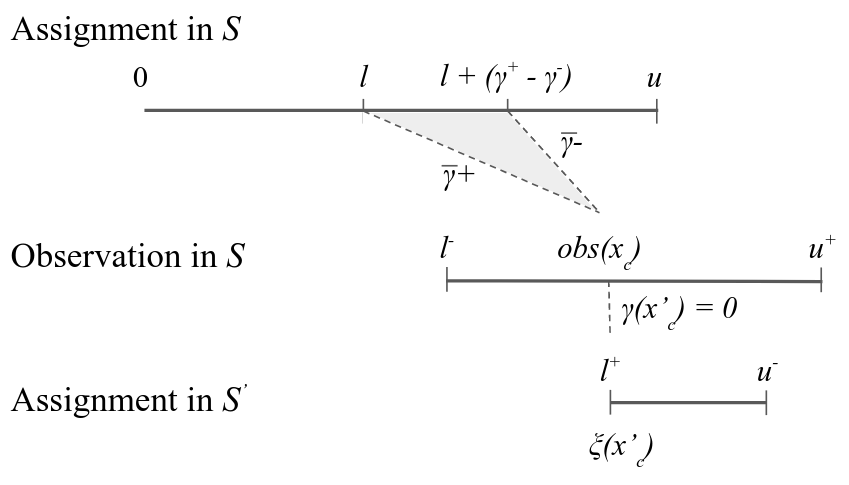
\includegraphics[width=3in]{images/viz-l-plus.png}
\caption{\label{fig:observations}Here, we show how the combination of \(\assign(x_{c})\) and \(\gammabar(x_{c})\) lead to an assignment of \(\assign(x'_{c})\) in \(S'\). We see the range \(\alpha \in [l, l + \gammabar^+(x_{c}) - \gammabar^-(x_{c})\) representing the earliest and latest assignments of \(\assign(x_{c})\) that could result in \(\obs(x_{c}) \in \assign(x'_{c}) \in [l^+(x_{c})\), l\^{}+(x\textsubscript{c})]\$. The grey region represents the range of possible observation delays, \(\gammabar(x_{c})\), supporting \(\assign(x'_{c}) \in [l^+(x_{c}), l^+(x_{c})]\).}
\end{figure}

The second category refers to the need for buffering and imagining events as a result of Lemma
\ref{lemma:main-tightening} using the execution strategy proven to be valid in Lemma
\ref{lemma:buffering-imagining}. There are three regimes of contingent event observations to address.

\begin{enumerate}
\item \(\obs(x_{c})  \in [l^-(x_{c}), l^+(x_{c}))\), ie. strictly earlier than the range
of \(\assign(x'_{c})\),
\item \(\obs(x_{c}) \in [l^+(x_{c}), u^-(x_{c})]\), ie. the range equivalent to \(x'_{c}\), and
\item \(\obs(x_{c}) \in(u^-(x_{c}), u^+(x_{c})]\), ie. strictly later than the range of
\(\assign(x'_{c})\).
\end{enumerate}

Note that we omit the \(-\gamma(x'_{c})\) term from Equation \ref{eqn:fixed-recording} in this analysis due
to the fact that \(\gamma(x'_{c}) = 0\) after applying Lemma \ref{lemma:main-tightening}.

Our execution strategy is to then make the following assignments during the FAST-EX real-time
update.

\begin{equation}
\assign(x'_c) = \begin{cases}
$l^+(x_{c})$  & \text{if } $\obs(x_{c}) \in [l^-(x_{c}), l^+(x_{c}))$ \textit{(buffering)} \\
$\obs(x_{c})$ & \text{if } $\obs(x_{c}) \in [l^+(x_{c}), u^-(x_{c})]$ \\
$u^-(x_{c})$  & \text{if } $\obs(x_{c}) \in (u^-(x_{c}), u^+(x_{c})]$ \textit{(imagining)}
\end{cases}
\end{equation}

In the first case, we cannot immediately schedule buffered events. It may be the case that there are
other unexecuted timepoints between \(\obs(x_{c})\) and \(l^+(x_{c})\). If we make an assignment at
\(l^+(x_{c})\), we would be preempting later timepoints, which would cause us to later make
assignments in the past, which invalidates our assumptions of partial history. Thus, we buffer
\(x'_{c}\) in the sense that we wait until \(l^+(x_{c})\) to assign \(\assign(x'_{c}) = l^+(x_{c})\).

In the last case, late observations are assigned to an earlier time. During execution, time is
always increasing. There is no need to wait to make an observation after \(u^-(x_{c})\). Instead, we
modify RTED generation, namely Equation \ref{eqn:rted1}, such that we dispatch \(x'_{c}\) at \(u^-(x_{c})\) if
it is not been observed before \(u^-(x_{c})\). Let \(U_{c}\) be the set of unobserved contingent
timepoints.

\begin{align}
\label{rted-with-ctg}
t_{x} &= \min\{-D(X, Z)~|~X \in U_{x}\} \\
t_{c} &= \min\{D(Z, X)~|~X \in U_{c}\} \\
t &= \min\{t_{x}, t_{c}\} \\
\chi_{x} &= \{X \in U_{x}~|~-D(X, Z) = t\} \\
\chi_{c} &= \{X \in U_{c}~|~D(Z, X) = t\} \\
\chi &= \chi_{x} \cup \chi_{c}
\end{align}

We see that RTEDs may now include unobserved (or unexecuted) contingent timepoints at their upper
bounds. Note that there is no need to distinguish between contingent events that are the result of
tightening during the fixed-delay transformation by applying Lemma \ref{lemma:main-tightening} and others.
We assume that the contingent constraints of the variable-delay STNU accurately reflect Nature. The
latest any other contingent event should be observed is their upper bound in \(S'\) and thus should
never be in the set of events, \(\chi\), of an executed RTED.

We have defined variable-delay execution strategies for when contingent events have infinite delay
and tightened constraints. The remaining category of contingent events is when a contingent event
has a finite, non-zero \(\gamma(x'_{c})\) in \(S'\). If that is the case, \(x'_{c}\) must have had fixed
observation delay in \(S\), Lemma \ref{lemma:emulating-fixed}, and can be scheduled normally after backing
out the observation delay with Equation \ref{eqn:fixed-recording}.

We have addressed the key issue of reconciling observations from \(S\) with the dispatchable form from
\(S'\). We now present a dispatcher and wrapper algorithms on top of FAST-EX that combine to add
robustness for variable observation delay.

\section{Experimental Analysis}
\label{sec:org5f3472d}
\label{sec:scheduling-experimental}

We first introduce an example which models a construction task on the lunar surface that will be
used to randomly generate STNUs with realistic constraints for benchmarking purposes. We then
describe benchmarks against the performance of the real-time FAST-EX update with the variable-delay
execution strategy, the dispatching routine, and observations. All benchmark code can be found at
\url{https://gitlab.com/enterprise/enterprise} in the \texttt{kirk-v2/benchmarks} directory.

\begin{figure}[htbp]
\centering
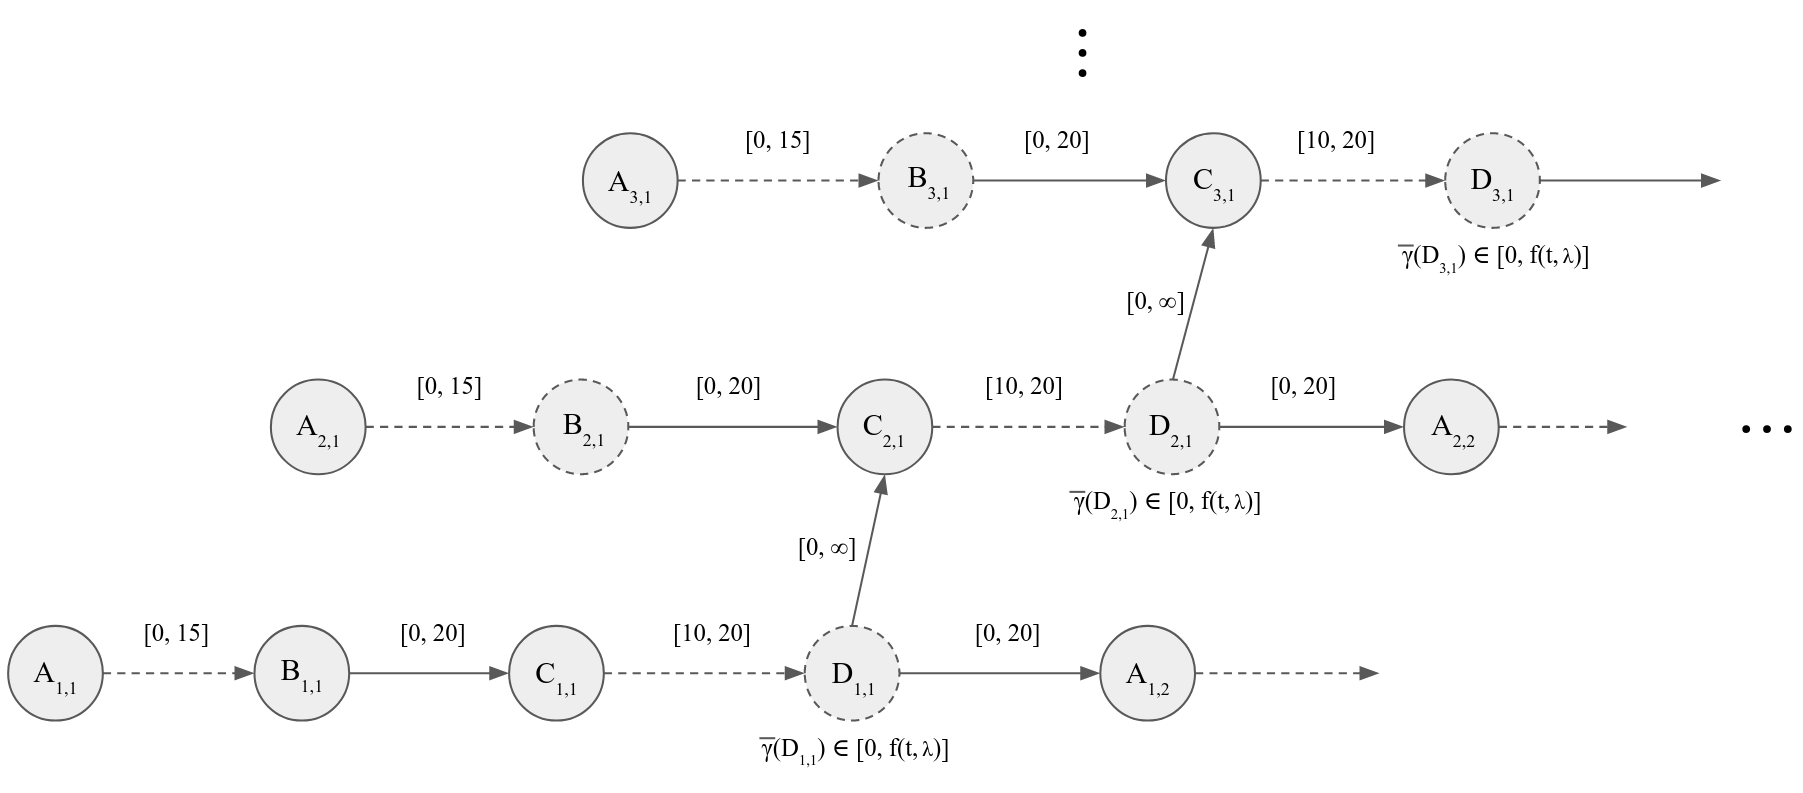
\includegraphics[width=1\textwidth]{images/dish-install-stnu.png}
\caption{\label{fig:dish-stnu}An STNU representing the installation and test of repeater antennas. Each row represents a single rover. The episode durations are representative of the bounds used in simulation.}
\end{figure}

It is possible that, before NASA is ready to grow the population of a lunar base, there is a need to
prepare a communications infrastructure near a habitat with a large grid of repeater antennas. This
scenario depicted with the STNU in Figure \ref{fig:dish-stnu} represents an installation task wherein \(i\)
rovers (mobile robot) are each installing \(j\) surface signal repeater antennas. During the activity,
every rover is responsible for installing one repeater. Each event, \(X\), is represented for the
\$i\$-th rover and \$j\$-th repeater as \(X_{i,j}\). All numbers in the figure are representative of the
minimum and maximum of the randomly generated constraints in the benchmarks.

The rovers work in parallel, with a \([0, \infty)\) requirement link from the start of the STNU to
each \(A_{i,1}\) (not shown). The first episode, \(\conedge{A_{i,j}}{B_{i,j}}{}\), represents traversing
to the site of the installation. We model traverses as uncontrollable due to the fact that crews are
embarking across unknown terrain. Once at the site, an antenna is installed as represented by
\(\edge{B_{i,j}}{C_{i,j}}{}\). Each repeater needs to have its configuration tested and confirmed
working by \(D_{i,j}\), represented by the edge \(\conedge{C_{i,j}}{D_{i,j}}{}\). Confirmation takes the
form of a request-response cycle to the ground. We model \(D_{i,j}\) as uncontrolled and with variable
delay because each antenna takes an unknown time to self-configure and the crew does not know when
they will receive a response from Earth that the repeater installation has been verified due to
uncertainty in communication. Bandwidth is limited, so we limit the number of repeaters
simultaneously sending requests to their configuration. We use the \(\edge{D_{i,j}}{C_{i+1,j}}{}\)
links to enforce that the start of the confirmation of the next repeater does not begin until after
the previous repeater's confirmation. Confirmations are required until we reach the last crew member
or the last activity. Once testing is complete, the rovers clean up their workstations,
\(\edge{D_{i,j}}{A_{i,j+1}}{}\) and then repeat the cycle until all antennas have been installed.

To perform the benchmarks, we generated variable-delay STNUs of increasing sizes with randomly
determined constraints as previously described. We immediately checked VDC of each STNU, and would
generate new STNUs of a given size until we found one that was confirmed to be VDC. We then
simulated scheduling and dispatching of the STNU with a faster-than-realtime clock. No driver was
present, so all real events were scheduled immediately.

These data were collected on an Intel i7-10710U 6c/12t mobile processor with 16GB of RAM in a
ThinkPad X1 Carbon Gen 7 laptop. All tests were run while the laptop was attached to wall power. The
code was written in Common Lisp and all benchmarks were run with Steel Bank Common Lisp version
2.0.1. To reduce the time spent running benchmarks, we scheduled multiple STNUs in parallel, with
each STNU being scheduled in its own thread.

The regressions below were performed using the Python packages \texttt{scipy} \citeprocitem{35}{[35]} and
\texttt{sklearn} \citeprocitem{36}{[36]}, then graphed with \texttt{matplotlib} \citeprocitem{37}{[37]}.

The implementation of the delay scheduler from which these data were collected has a bug that we
have been unable to identify. We have only seen the bug surface with STNUs with more than about 50
events. The bug takes effect when observing a contingent event, \(x_{c}\), which has incoming
contingent constraint \([l, u]\). If we observe \(x_{c}\) at some time \(t\), where \(l \leq t < u\), the
Dijkstra SSSP subroutine may unexpectedly find a negative edge and raise an error. We have been
able to replicate the problem for specific STNUs with specific observations, and, as of the time of
this writing, we are still investigating the cause. We do not believe it meaningfully impacts the
validity of the benchmarks below.

\subsection{Scheduling}
\label{sec:orge444d26}

We start with the runtime performance of schedule updates. There can be runtime variance for each
individual call to the scheduling update routine, so we focus on the total time spent scheduling all
events in the STNU. According to the FAST-EX algorithm, the total runtime is dominated by the \(O(N
\log N)\) runtime of Dijkstra SSSP, where \(N\) is the total number of events. Thus, the total runtime
to schedule every event in an STNU is \(O(N^{2} \log N)\) \citeprocitem{15}{[15, p. 144]}. Given the
changes we made to FAST-EX are also dominated by Dijkstra SSSP, we expect to see the same runtime
performance here.

Figure \ref{fig:runtime-scheduling-sub-300} clearly shows that the total time spent scheduling STNUs with
\(N \leq 300\) follows \(O(N^{2} \log N)\) as expected, with a coefficient of determination for the
regression of \(R^{2} = 0.995\).

\begin{figure}[htbp]
\centering
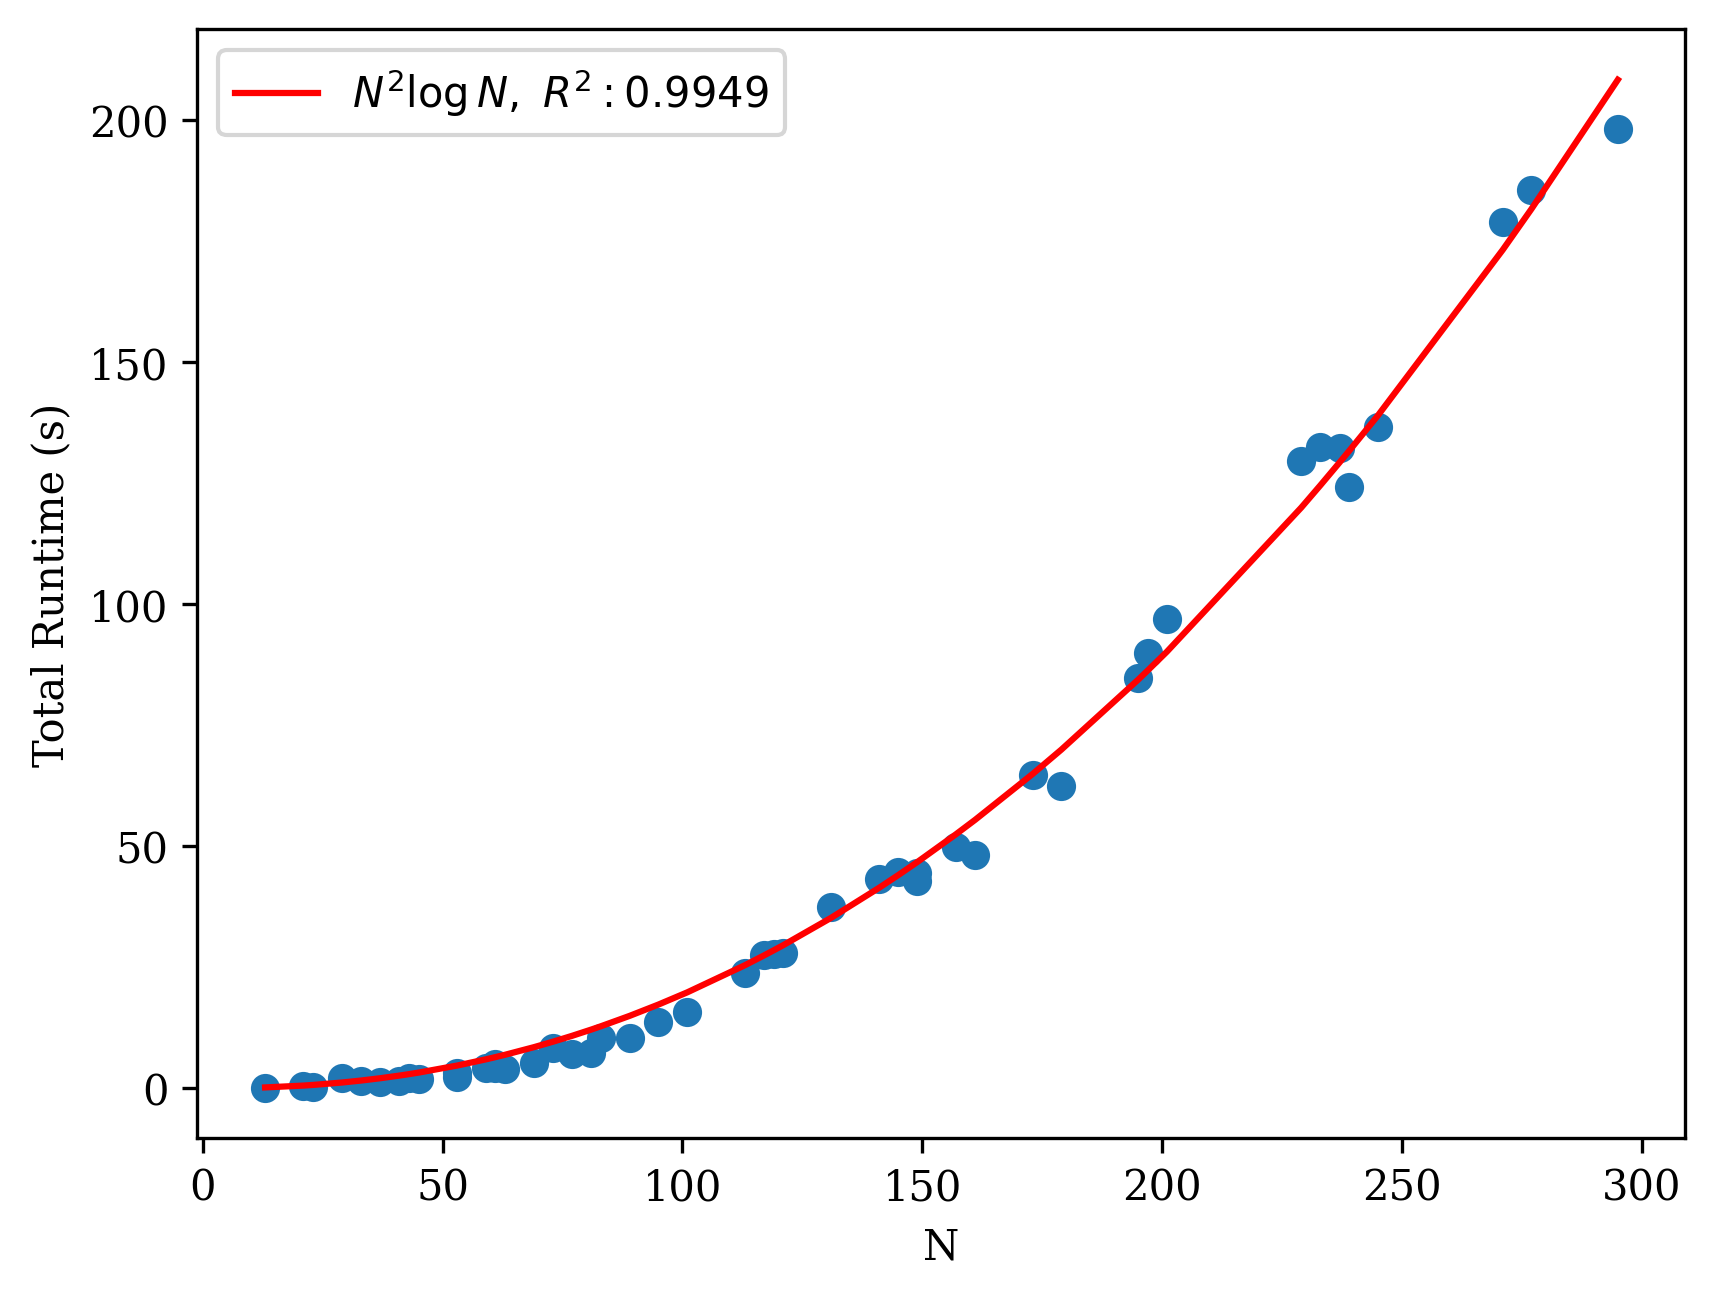
\includegraphics[width=0.8\textwidth]{images/scheduling-total-runtime-sub-300.png}
\caption{\label{fig:runtime-scheduling-sub-300}Total runtime data for scheduling all events in VDC STNUs where \(N \leq 300\).}
\end{figure}

If we expand the size of STNUs to \(N \leq 600\), then we see the total runtime correspond less
closely with \(O(N^{2} \log N)\), as can be seen in Figure \ref{fig:runtime-scheduling-aggregate}. We
believe the deviation is due to programming language features in lisp outside of our control, such
as automated memory management.

\begin{figure}[htbp]
\centering
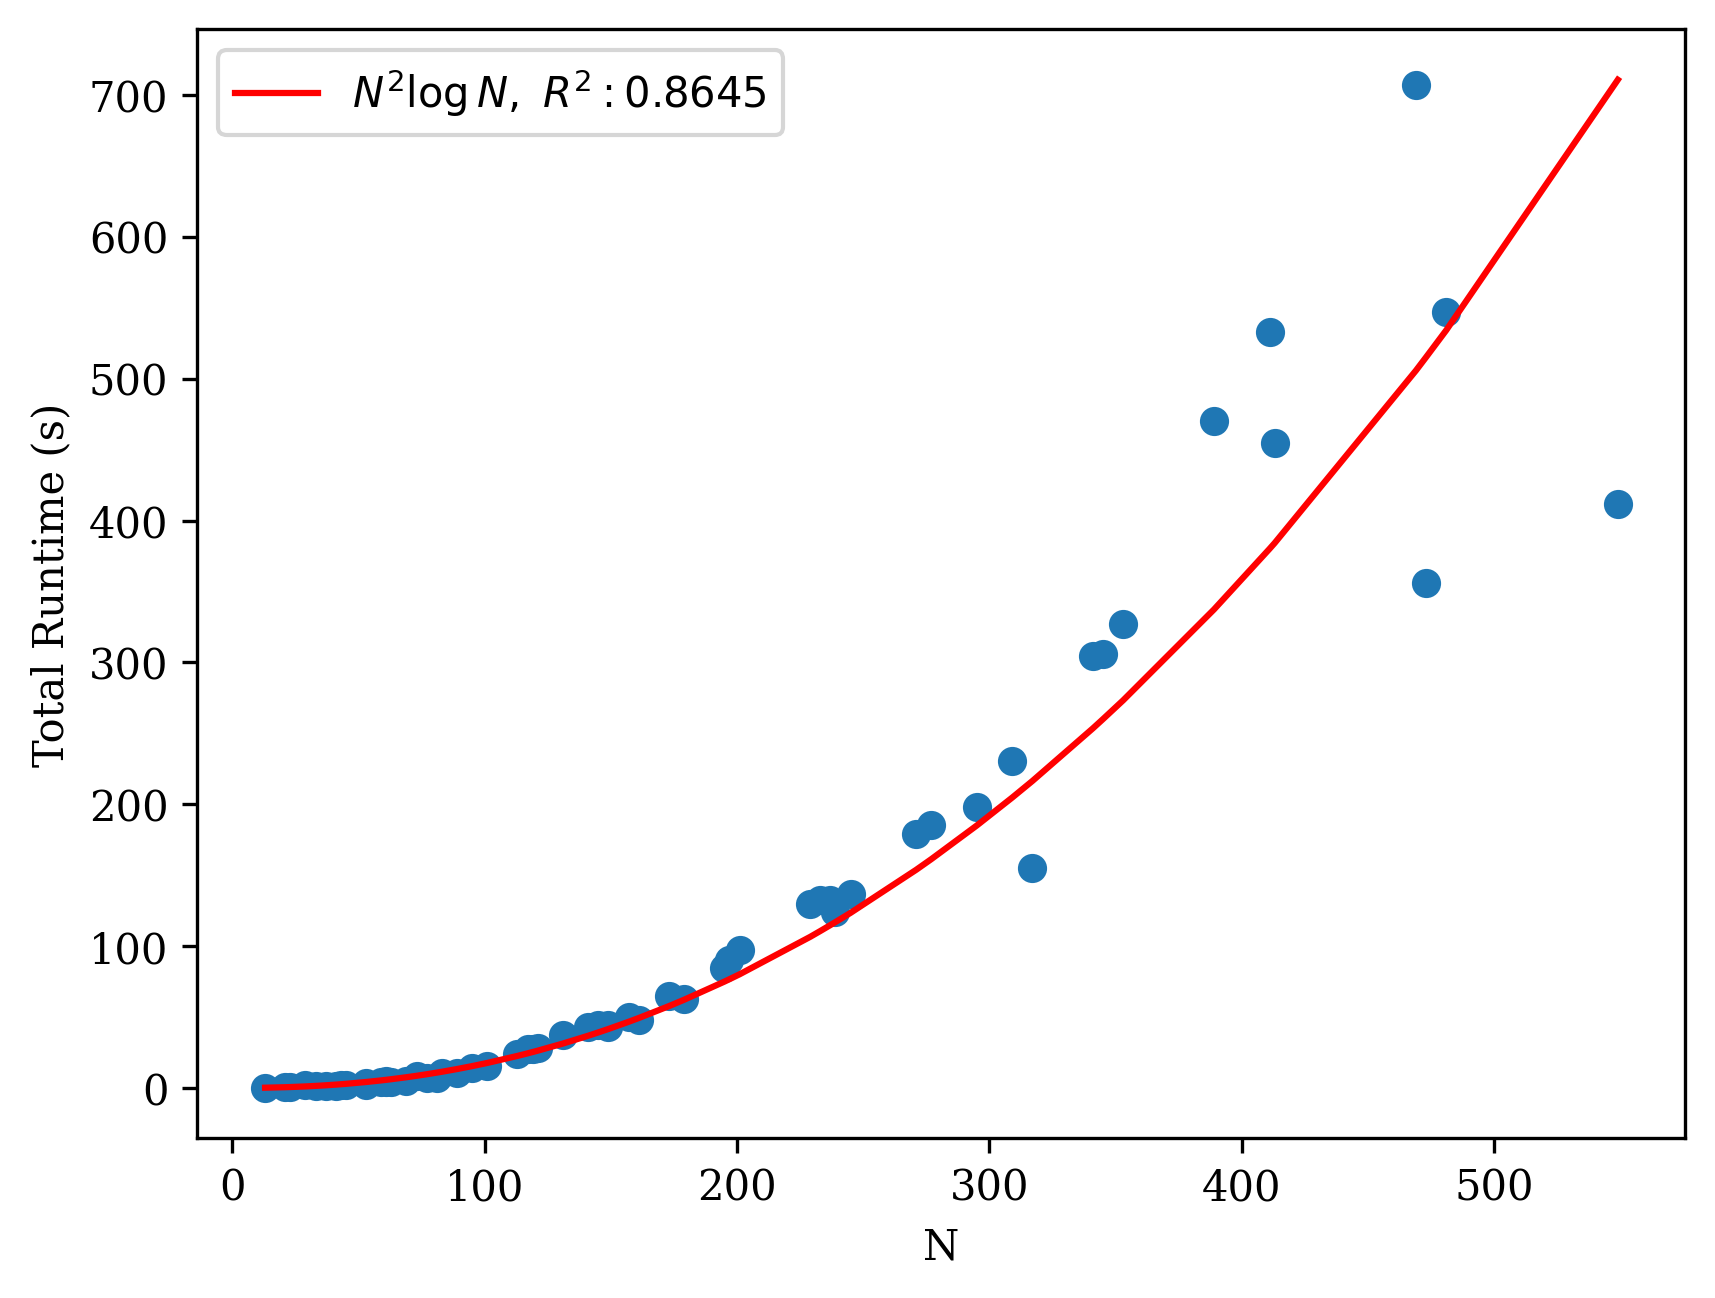
\includegraphics[width=0.8\textwidth]{images/scheduling-total-runtime-all.png}
\caption{\label{fig:runtime-scheduling-aggregate}Total runtime data for scheduling all events in VDC STNUs where \(N \leq 600\).}
\end{figure}

\subsection{Event Observations}
\label{sec:org7c9153f}

Next, we examine the runtime characteristics of event observations. While generating VDC STNUs, we
also collected possible ranges of time to observe the confirmation event. As scheduling progressed,
we automatically triggered observations of the confirmation event at a time randomly selected within
the range given.

Contingent event observations are made much less frequently than scheduling. While we must schedule
every event in an STNU, our benchmarking procedure will only observe a small fraction of the events.
As a result, sample sizes are small. Given event observations are dominated by the call to FAST-EX
for a scheduling update, we expect to see runtimes on the order of \(O(N \log N)\). However, the data
in Figure \ref{fig:runtime-observations-aggregate} show significant deviation from it. Given that the
method call to observe events is a thin wrapper around a FAST-EX update, we believe the error of
this graph is due to small sample sizes.

\begin{figure}[htbp]
\centering
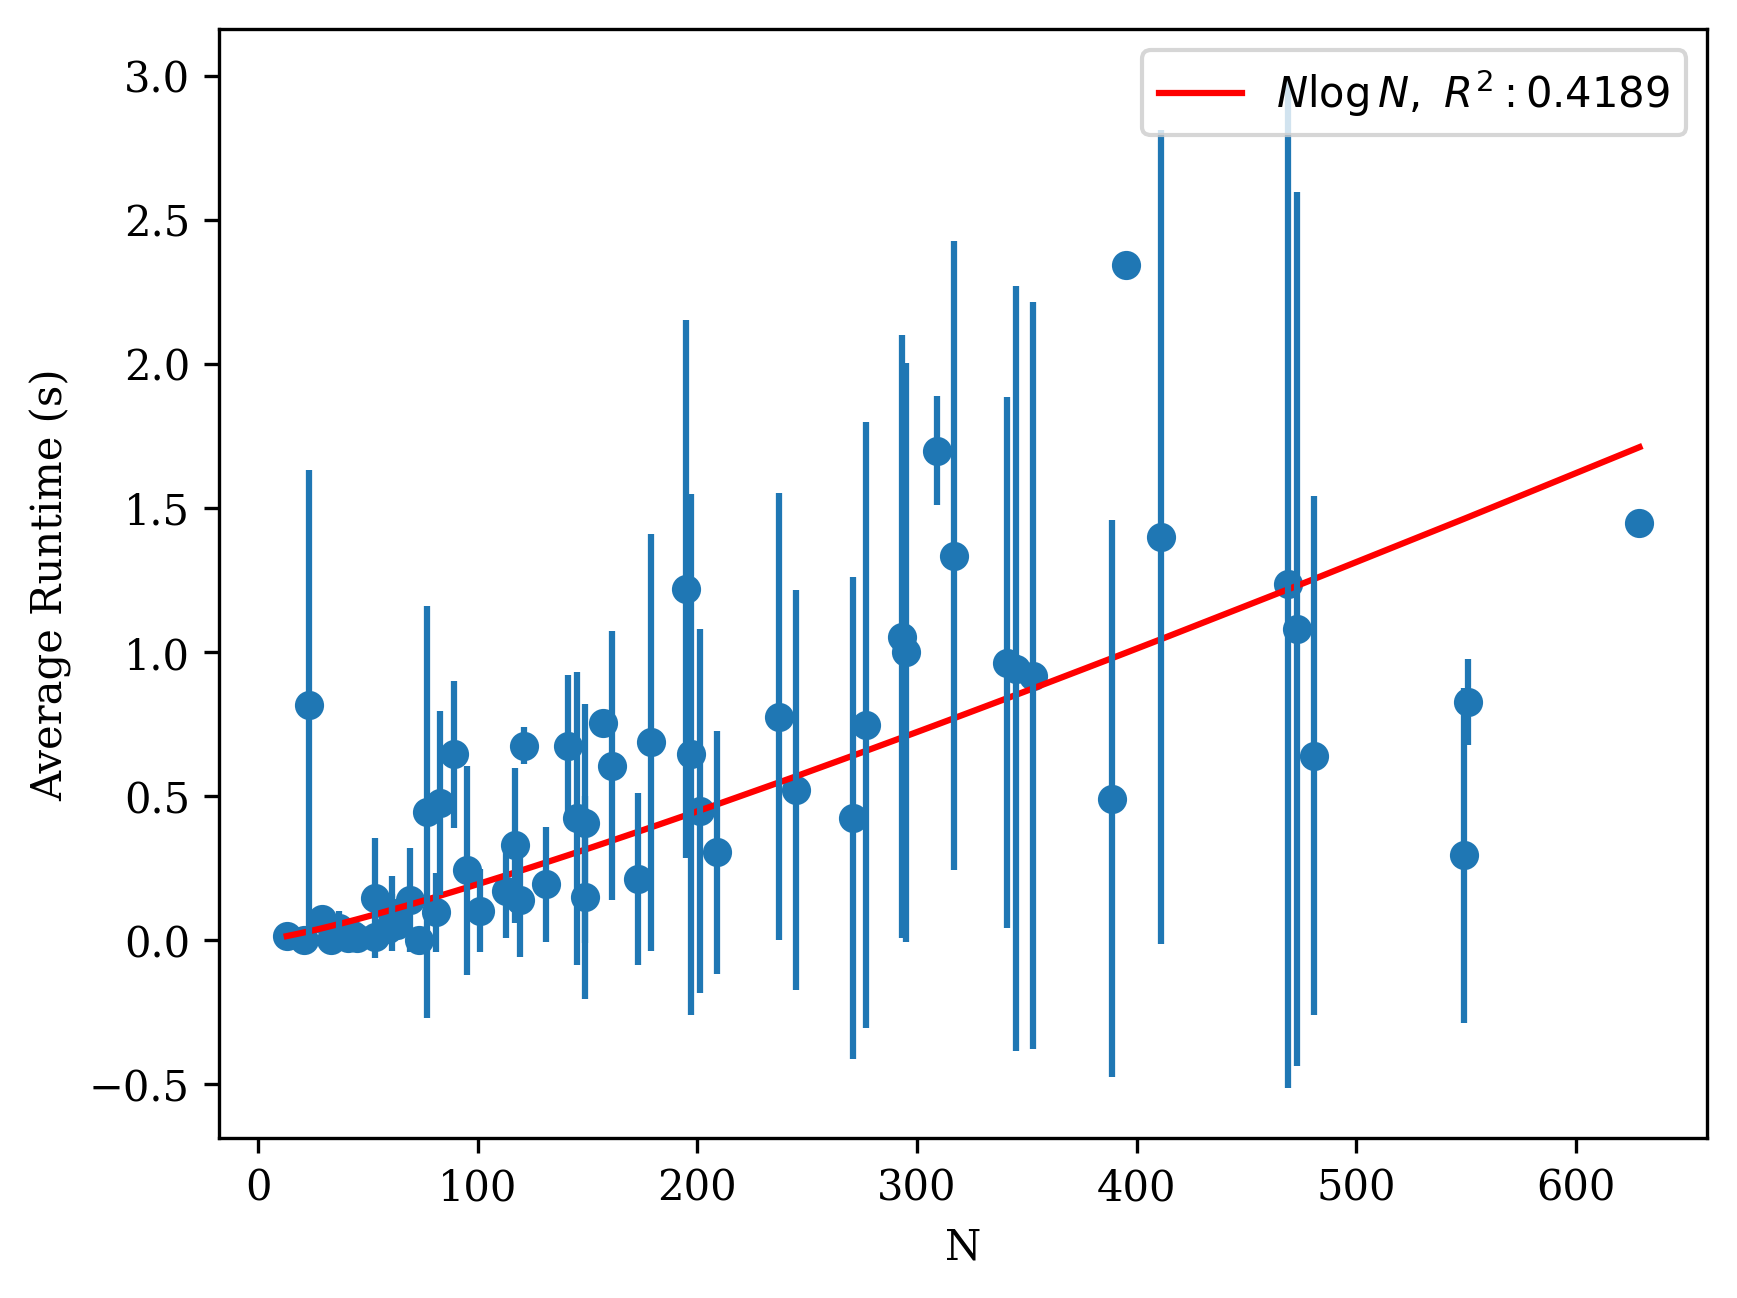
\includegraphics[width=0.8\textwidth]{images/observations-avg-runtime.png}
\caption{\label{fig:runtime-observations-aggregate}Average runtime data for observing events in VDC STNUs. Error bars represent standard deviation.}
\end{figure}

\subsection{Dispatching}
\label{sec:orgb83c2b9}

Finally, we benchmark action dispatching. In our simulated environments for dispatching, we run the
dispatcher function as described in Algorithm \ref{alg:dispatcher-inner} twice per simulated second. (We
run it twice in the event that scheduling an event enables us to dispatch other actions immediately.
If we ran Algorithm \ref{alg:dispatcher-inner} once per second, the newly enabled events would then be
dispatched a second late.)

Given every event will be scheduled once using the FAST-EX update, FAST-EX updates will dominate the
total runtime of dispatching. As seen in Figure \ref{fig:runtime-tick-aggregate}, the total runtime of all
calls to Algorithm \ref{alg:dispatcher-inner} indeed follows \(O(N^{2} \log N)\).

\begin{figure}[htbp]
\centering
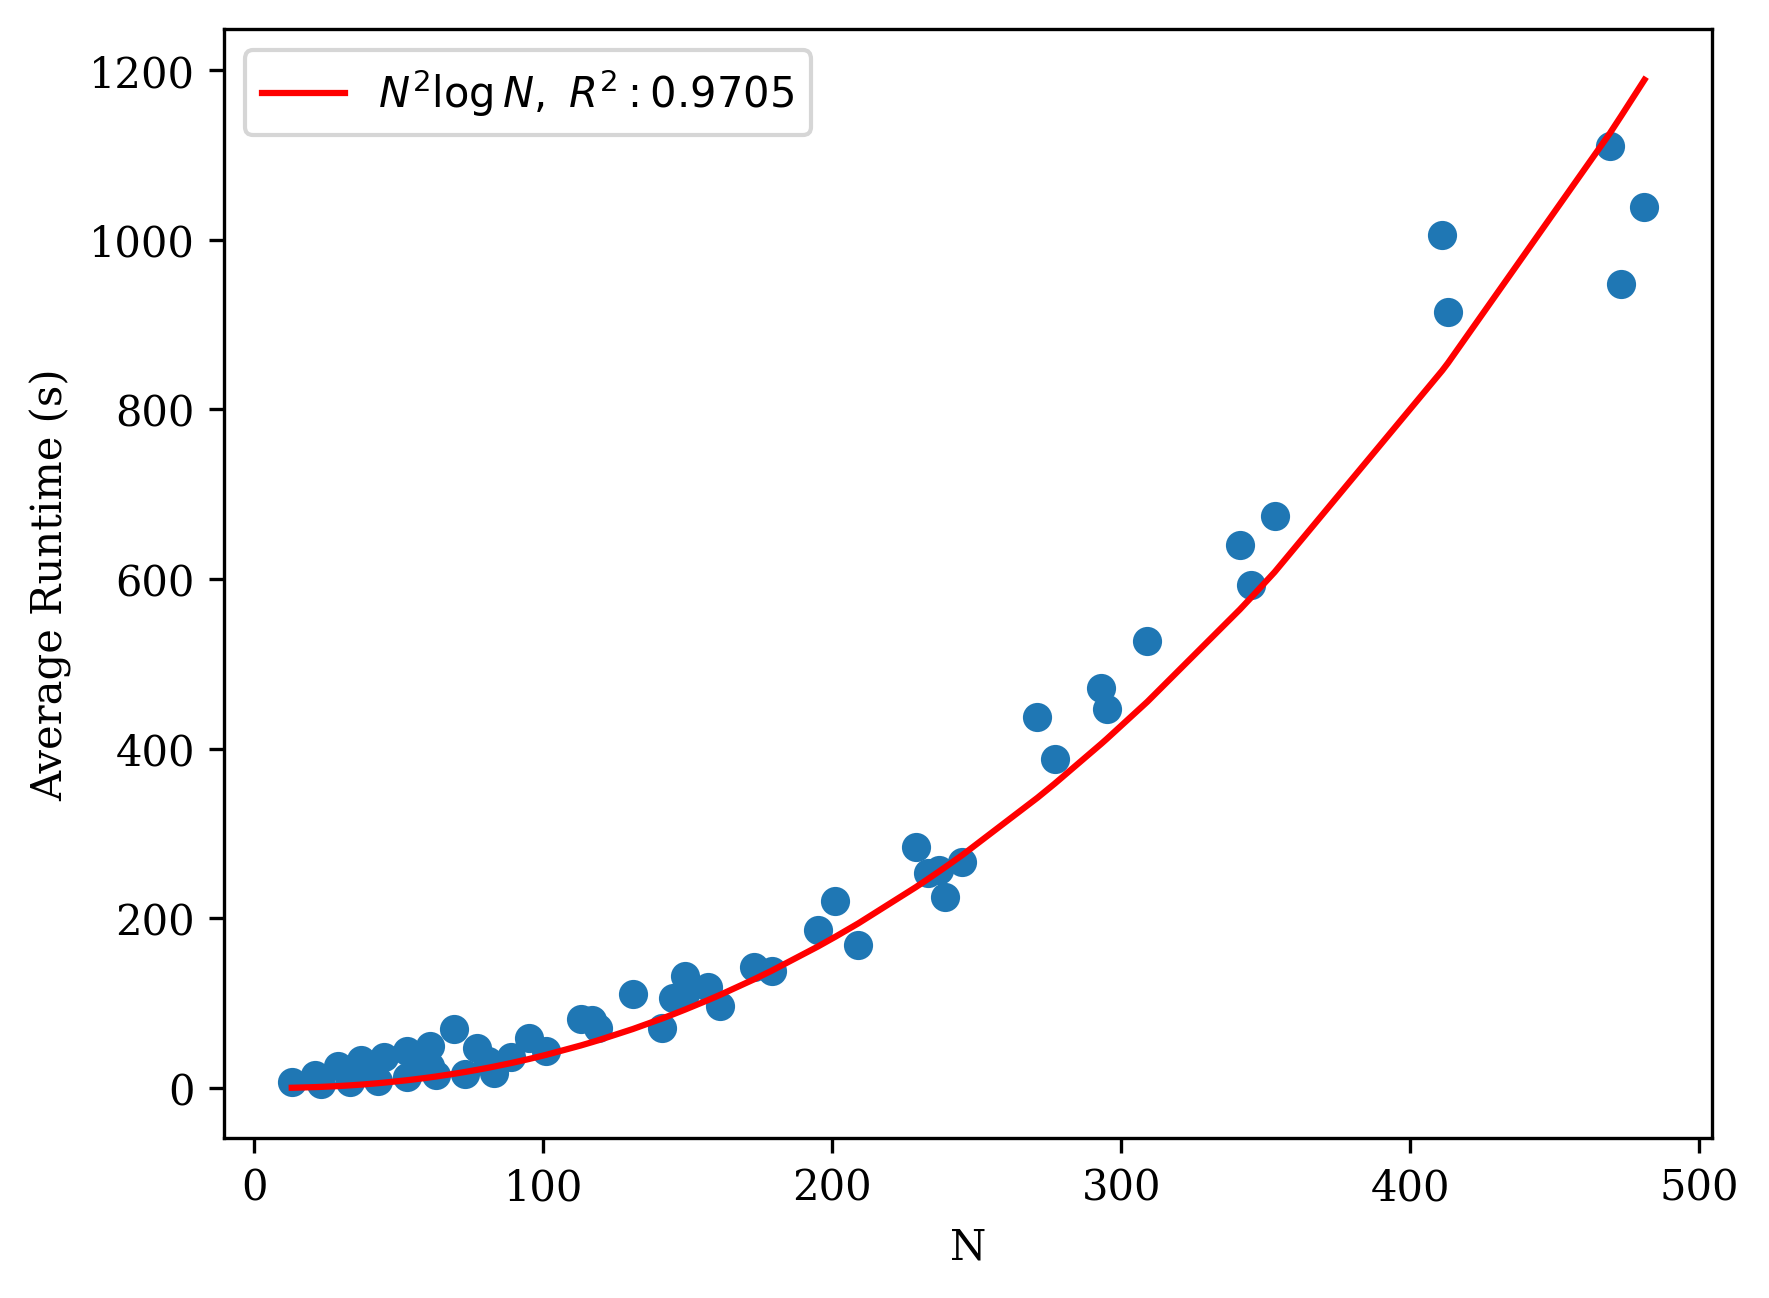
\includegraphics[width=0.8\textwidth]{images/tick-total-runtime.png}
\caption{\label{fig:runtime-tick-aggregate}Average runtime data for running Algorithm \ref{alg:dispatcher-inner}.}
\end{figure}

\chapter{An Executive for Scheduling with Observation Delay}
\label{sec:org7fe1f68}
\label{ch:technical-executive}

A delay scheduler is only useful if there is a system capable of dispatching the actions associated
with RTEDs. A delay scheduler could be integrated as a subsystem for a digital assistant, if such a
digital assistant has a means for surfacing RTEDs in a useful. Instead, for this thesis, we chose to
integrate with a high-level task and motion planner, \emph{Kirk} \citeprocitem{38}{[38]}. Kirk is a
complete, end-to-end executive in that it can take human-friendly problem specifications as input
and send commands to hardware as output.

At a high-level, Kirk operates by first taking a description of the problem domain as written by
domain experts, which should include the constraints, agent dynamics, environment, and starting and
goal states of the problem at hand. Kirk then generates state plans, which consist of episodes that
organize the occurrence of events as activities. State plans may include temporal constraints and
non-temporal constraints, such as classical planning preconditions and effects. Kirk checks plans
for consistency using an optimal satisfiability (OpSAT) solver \citeprocitem{39}{[39]}. Next, it
elaborates temporal plan networks (TPNs) \citeprocitem{40}{[40]} to sub-executives when it encounters
constraints and goals it cannot plan against directly. Finally, it dispatches event schedules and
motion plans to hardware. For the purpose of this thesis, we focus on Kirk's capability to create
delay STNUs from state plans, then dispatch actions online after a plan has been generated.

Below, we present an instantiation of Kirk, \emph{Delay Kirk}, designed to dispatch actions from state
plans with uncertain observations. A delay scheduler lives at the core of Delay Kirk, with a new
component, a \emph{delay dispatcher} taking responsibility for translating RTEDs into actions in the real
world. We start by defining a delay dispatcher, which plays a key role in enabling delay scheduling.
Next, we present a high-level overview of Kirk's architecture. Finally, we define necessary
components of an input language, the Reactive Model-Based Programming Language (RMPL), used to
represent constraints and action models for Delay Kirk. At the end of this Chapter, we present
experimental results on the performance of the delay dispatcher.

\section{Dynamic Dispatching of STNUs with Observation Delay}
\label{sec:org2e577ae}
\label{sec:delay-scheduler}

We assume that events in an STNU map 1:1 to actions in the real world. To put the design of the
dispatcher in context, it is worth considering what events may look like. In the case of a robotic
agent, requirement events may represent the instantaneous timepoints when motion plans begin, while
contingent events could be anything from the completion of said motion plans to the receipt of
\texttt{PROCEED} messages from a third party. For a human, requirement events could be presented in a
mission timeline as the start of planned actions such as the collection of scientific samples. The
end of a sampling activity would then be a contingent event. Or contingent events could be the
actions performed by other agents, like say another astronaut on an EVA, with whom temporal
constraints are shared. In both the case of the robot and the human, a robust dispatcher should take
into consideration that passing a message to the agent telling it to execute a requirement event
does not cause the event to occur instantaneously. Put in other words, dispatching is not the same
as assignment. A robot may require offline processing before it executes the motion plan. Or a human
may need to acknowledge that they have started the activity their mission timeline has told them to
perform. Neither is a problem, though, for our chosen formalism for temporal reasoning so long as
each requirement event is assigned at some point within their constraints in the STNU. In our view,
the dispatcher is responsible for ensuring requirement constraints are met by both monitoring the
real-world and interfacing with hardware to cause actions to be performed.

\begin{figure}[htbp]
\centering
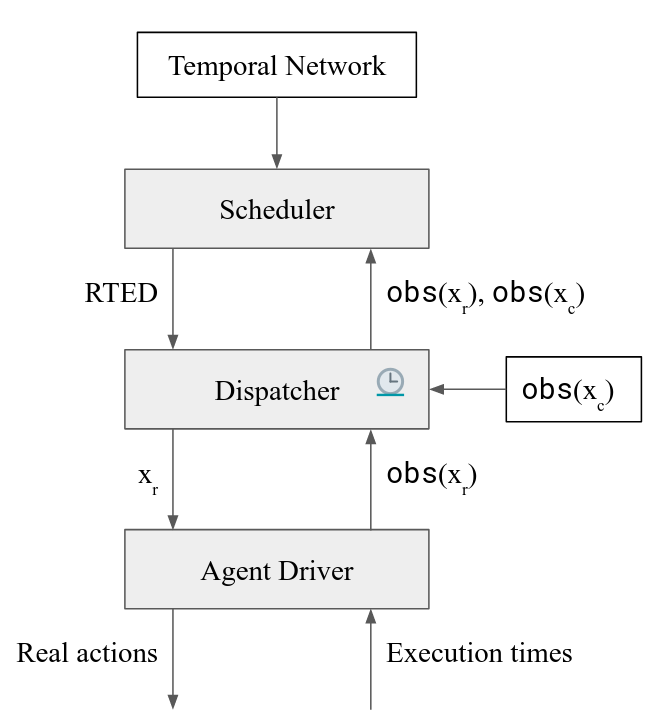
\includegraphics[width=0.6\textwidth]{images/architecture.png}
\caption{\label{fig:executive-dispatching-architecture}A more detailed view of the delay dispatcher architecture.}
\end{figure}

We finally introduce a third component, the \emph{driver}, that can interpret dispatched events and cause
some action to be performed in an exogenous system. For instance, if Delay Kirk is controlling a
robotic arm, the driver might be responsible for forming and publishing ROS messages when the
dispatcher dispatches an event. If Delay Kirk is managing an astronaut's EVA schedule, the driver
might be responsible for causing a heads up display to alert the astronaut to start their sample
collection procedure.

In this Section, we contribute a set of algorithms for building the dispatcher for a robust
executive that can reason over observation delay and safely enact the actions symbolized in
requirement events in the real world. Dynamic dispatching is designed around the two interfaces of
scheduling - the input of partial schedules and output of RTEDs. As such, we focus on the
interpretation, management, and flow of RTEDs in Section \ref{sec:dynamic-dispatching} and observing
events in Section \ref{sec:event-observations}. But first, we present a novel view on RTEDs that is
required for dispatching events to real hardware in Section \ref{sec:real-vs-noop-events}.

\subsection{Guaranteeing Agents Receive Actionable Events}
\label{sec:orgc3768e4}
\label{sec:real-vs-noop-events}

We take the view that events in an STNU may be interpreted as commands by the driver. It is improper
to knowingly send an invalid command. Accordingly, the driver must never receive a dispatched event
that cannot be mapped to a corresponding action in its exogenous system. As such, it is the
dispatcher's responsibility to filter events in order to only dispatch valid commands to the driver.

In a variable-delay STNU, there are events that need to be executed by the driver and there are
events that do not. We call these \emph{real} and \emph{noop} (``no operation'') events. Both contingent \emph{and}
requirement events may fall into either category. Below, we present our rationale for the
distinction between real and no-op events, and how we modify real-time execution decisions
accordingly.

To start, imagined contingent events are no-ops. They are assignments we artificially perform with
no corresponding real-world action, and solely exist to maintain the controllability of the
fixed-delay dispatchable form. Imagined events should never be dispatched to a driver.

There are requirement events that are also no-ops. Consider the process of normalization of an STNU
\citeprocitem{31}{[31]}. While building the labeled distance graph during a DC check, we rewrite
contingent links such that their lower bounds are always \(0\). For instance, for a contingent event
\(C\) and free event \(E\), \(C - E \in [l, u]\), during normalization we create a new requirement event,
\(C'\), fixed at the lower bound of the contingent link, and then shift the bounds of the contingent
link to start at 0 while maintaining the original range, \(u - l\). This results in two constraints:
\(E - C' \in [l, l]\) and \(C - C' \in [0, u - l]\) that still reflect the original contingent link's
semantics.

Importantly, the requirement events representing the normalized lower bounds of contingent events
are in the dispatchable form for dynamic scheduling because we draw the AllMax graph directly from
the DC check. To a scheduler, there is no distinction between the semantics of a real event, as
modeled by a human planner writing an STNU for an agent to execute, and \(C'\), an artifact of
checking controllability. Both are modeled in the AllMax distance graph forming the basis of RTED
generation. However, an agent does not need to execute any task in the outside world to satisfy \(E -
C'\). Thus, we make the following addendum to the definition of RTEDs.

\newcommand*{\eventnoop}{\mathit{event}\textsf{-}\mathit{noop}}
\newcommand*{\eventnoops}{\mathit{event}\textsf{-}\mathit{noops}}

\begin{defn}
\textbf{Event-No-op Pair}

An \emph{Event-No-op Pair}, \(\eventnoop\), is a two-tuple, \(\langle x, \mathit{noop} \rangle\),
where:
\begin{itemize}
\item \(x\) is an event in \(X_{e} \cup X_{c}\),
\item \emph{noop} is a boolean, where if true, the event cannot be interpreted by the driver, else the event
is a valid command.
\end{itemize}
\end{defn}

\begin{defn}
\label{def:rted-op}
\textbf{RTED with Operational Distinction}

A \emph{Real-Time Execution Decision with Operational Distinction} is a two-tuple \(\langle t,
\eventnoops \rangle\), where:
\begin{itemize}
\item \(t\) is a time with domain \(\mathbb{R}\),
\item \(\eventnoops\) is a set of \(\eventnoop\) pairs to be executed at time \(t\).
\end{itemize}
\end{defn}

For convenience and simplicity, and given the similarities between RTED and RTED with Operational
Distinction, future references to RTEDs will always refer to RTEDs with Operational Distinctions.

\subsection{Dynamic Event Dispatching}
\label{sec:orge8cd445}
\label{sec:dynamic-dispatching}

The dynamic dispatcher runs the main loop of the executive's temporal reasoning routine. It consists
of a dispatching routine and some type of outer loop monitoring it. The dispatching routine,
Algorithm \ref{alg:dispatcher-inner}, is responsible for retrieving the latest RTEDs and firing driver
commands when the clock indicates that the agent has reached time \(t\) corresponding to the latest
RTED. The outer loop allows the dispatching routine to run until the scheduler reports there are no
requirement events remaining.

The dispatcher requests RTEDs with blocking synchronous calls, while the dispatcher and driver
communicate asynchronously. The dispatcher spawns a thread to make non-blocking calls to the
driver's interface to execute events. The dispatcher and driver also share a FIFO queue that the
driver can append messages to indicating the successful execution of events.

We now provide a walkthrough of the dynamic dispatching algorithm. For simplicity's sake, the term
\emph{schedule} here is shorthand for whatever data structures the scheduler uses to generate RTEDs.
\emph{Updating the schedule} refers to running the fixed-delay FAST-EX update, Algorithm
\ref{alg:fast-ex-fixed-obs}, using the variable-delay execution strategy from Section
\ref{sec:delay-scheduling}.

The interaction between the dispatching routine and monitoring loop is limited. Algorithm
\ref{alg:dispatcher-inner} returns a Boolean indicating whether there are executable events remaining.
Here, the monitoring loop is a simple \texttt{while} that repeats until it receives \texttt{false} from the inner
loop. Otherwise, the only communication between the dispatching routine and outer loop is a variable
containing the last RTED that was generated but not executed. The outer loop creates the variable
and passes it by reference to the dispatching routine, which is free to use or modify the variable
as it sees fit.

We break the dispatching routine into three distinct phases.

\begin{enumerate}
\item Receive execution confirmation from the driver.
\item Collect an RTED and confirm the clock time matches RTED time \(t\).
\item If there is an RTED:
\begin{enumerate}
\item send executable events to the driver, else
\item immediately assign all \emph{no-op} events to the current time.
\end{enumerate}
\end{enumerate}

Our goal in the dispatching routine is to dispatch events to the driver only after updating the
schedule, collecting an up-to-date RTED, and confirming we are within the time window of the RTED.
The routine will exit before reaching the dispatch step if any conditions are not met.

For the first step, we ask the scheduler if there are any remaining executable events. If there are
none, we return \texttt{false} to signal the loop's termination, otherwise we continue.

Next, we check the FIFO queue for any event execution messages returned from the driver. The
presence of a message would indicate that the driver has successfully executed a free event. We
iteratively pop messages off the queue and update the schedule with the events and execution time
contained in each message. Note that the scheduler update is a blocking operation because we need an
up-to-date schedule to guarantee future RTEDs are consistent. We then invalidate the last RTED
generated.

The second step starts once we have popped all messages from the driver off the queue. If we do not
have a valid RTED from the last iteration of the routine, we ask the scheduler for one and save it
to the referenced variable from the outer loop. Given that we interact with the driver
asynchronously, it is possible that the current RTED is one that has already been sent to the driver
but we have yet to receive an acknowledgment message confirming its execution. If so, there is
nothing to do so we return \texttt{true}.

Lastly, we compare the suggested time in the RTED against the clock's elapsed time. Given the
relationship between the scheduler, routine, and driver, we do not assume that dispatched events are
executed instantaneously by the driver. We know that execution contends against delays such as the
computational time in simply calling a function, to network latency, to robotic hardware that takes
a moment to interpolate a motion plan from waypoints. In some contexts, it may make sense to preempt
execution by dispatching events some small amount of time \emph{before} the clock time reaches the RTED
execution window. We call this preemption time \(\epsilon\), where \(\epsilon \in \mathbb{R}^{\geq 0}\).
Thus, we dispatch events, signaled by \texttt{dispatch-p}, when \(\texttt{dispatch-p} = (t_{\mathit{RTED}} -
t_{\mathit{clock}} \leq \epsilon)\). If \(\epsilon = 0\), the dispatcher is not allowed to preemptively
dispatch events before the RTED time. We allow the human operator to choose an \(\epsilon\) that is
consistent with the operational context for the driver.

If \texttt{dispatch-p} is \texttt{false}, we are too early to execute the RTED and so the loop returns \texttt{true}.
Otherwise we continue.

Once we reach the third stage, we are guaranteed to be able to safely dispatch events because (1) we
have confirmed that the RTED we have in hand has unexecuted events that have never been dispatched,
and (2) that we are in a time window that the scheduler has told us is consistent with the STNU's
constraints. Going forward, we take advantage of the operational distinction we added to
Hunsberger's RTEDs in Definition \ref{def:rted-op}. Using the \emph{no-op} property of each \(\eventnoop\) pair
in the RTED, we filter the \(\eventnoop\) pairs into a set of \emph{no-op} events and a set of real events.
In the event that a contingent event and its normalized lower bound are to be scheduled at the same
time, we schedule the \emph{no-op} events first. The real events are then asynchronously sent to the
driver.

Finally, because events were dispatched, the dispatching routine returns \texttt{true}.

\begin{algorithm}
\SetAlgoLined
\SetKwComment{Comment}{//}{}
\SetKwFunction{Return}{return}
\SetKwInput{Input}{Input}
\SetKwInput{Output}{Output}
\SetKwInput{Algorithm}{\textsc{Dynamic Dispatching Outer Loop}}
\SetKwInput{Initialize}{Initialization}
\SetKwIF{If}{ElseIf}{Else}{if}{then}{else if}{else}{endif}
\SetKw{Continue}{continue}

\Indm

\Initialize{$\mathit{RTED_{\mathit{last}}} \gets \varnothing$}

\Indp
\Algorithm{}
\Indp

\While{Calling inner loop with $\mathit{RTED_{\mathit{last}}}$ returns $\textbf{true}$} {
    \Continue
}
\caption{The outer loop of the dynamic dispatching algorithm.}
\label{alg:dispatcher-outer}
\end{algorithm}

\begin{algorithm}
\SetAlgoLined
\SetKwComment{Comment}{//}{}
\SetKwFunction{Return}{return}
\SetKwInput{Input}{Input}
\SetKwInput{Output}{Output}
\SetKwInput{Algorithm}{\textsc{Dynamic Dispatching Routine}}
\SetKwInput{Initialize}{Initialization}
\SetKwIF{If}{ElseIf}{Else}{if}{then}{else if}{else}{endif}

\Indm
\Input{$\mathit{Scheduler}$; $\mathit{Driver}$; FIFO queue, $\mathit{Queue}$; $\mathit{RTED_{\mathit{last}}}$; $\epsilon$;}
\Output{Boolean whether the outer loop should continue}

\Initialize{$\mathit{events}_{\mathit{real}} \gets$ \{\}; $\mathit{events}_{\mathbf{noop}} \gets$ \{\};}

\Indp
\Algorithm{}
\Indp

\If{$\mathit{Scheduler}$ has no more unexecuted events} {
    \Return $\mathtt{false}$\;
}

\For{$\mathit{message}$ in $\mathit{Queue}$} {
    Pop $\mathit{message}$\;
    \For{$\mathit{event}, t_{\mathit{execution}}$ in $\mathit{message}$} {
        Set $\assign(\mathit{event}) = t_{\mathit{execution}}$ in $\mathit{Scheduler}$\;
    }
    $\mathit{RTED_{\mathit{last}}} \gets \varnothing$\;
}

$\mathit{RTED} \gets$ a new RTED from $\mathit{Scheduler}$; \Comment{Equations \ref{eqn:rted-chi} and \ref{eqn:rted-t}}

\If{$\mathit{RTED} = \mathit{RTED}_{\mathit{last}}$} {
    \Return $\mathtt{true}$\;
}

$\mathit{RTED}_{\mathit{last}} \gets \mathit{RTED} $\;

\If{$t_{\mathit{RTED}} - t_{\mathit{current}} > \epsilon$} {
    \Return $\mathtt{true}$\;
}

\For{$\eventnoop$ pair in $\mathit{RTED}_{\eventnoops}$} {
    \eIf{$\eventnoop[noop]$ is \textbf{true}} {
        Add $\eventnoop[x]$ to $\mathit{events}_{\mathbf{noop}}$\;
    } {
        Add $\eventnoop[x]$ to $\mathit{events}_{\mathit{real}}$\;
    }
}

\For{$\mathit{event}$ in $\mathit{events}_{\mathbf{noop}}$} {
    Set $\assign(\mathit{event}) = t_{\mathit{RTED}}$ in $\mathit{Scheduler}$\;
}

Asynchronously send all $\mathit{events}_{\mathit{real}}$ to the $\mathit{Driver}$\;

\Return $\mathtt{true}$\;

\caption{The dynamic dispatching routine.}
\label{alg:dispatcher-inner}
\end{algorithm}

The biggest factor for the performance of the dispatching routine, Algorithm
\ref{alg:dispatcher-inner}, is updating the schedule. Assuming the \emph{Scheduler} is the Delay Scheduler
described in Section \ref{sec:delay-scheduler}, then performing an assignment of an event will trigger the
FAST-EX update that runs in \(O(N^{3})\) \citeprocitem{15}{[15, p. 144]} with the number of events in the
STNU. In the worst case, the dispatcher confirms that all events in the STNU have arrived at the
same time, whether as messages from the driver in the FIFO queue, or RTED \texttt{noop} events. Each event
would trigger a schedule update. Thus, the dynamic dispatching routine runs in \(O(N^{4})\) in the
worst case.

\subsection{Observing Contingent Events}
\label{sec:orgc1c6819}
\label{sec:event-observations}

The dispatcher relays contingent event observations to the scheduler. In the base case, when a
contingent event is observed, the dispatcher updates the schedule with the event and current clock
time.

If the observed event is contingent and arrived earlier than its lower bound, then the dispatcher
will save the event in a \texttt{buffered-events} hash-table for the lower bound.

\subsection{Experimental}
\label{sec:org4456444}

Finally, we benchmark action dispatching. In our simulated environments for dispatching, we run the
dispatcher function as described in Algorithm \ref{alg:dispatcher-inner} twice per simulated second. (We
run it twice in the event that scheduling an event enables us to dispatch other actions immediately.
If we ran Algorithm \ref{alg:dispatcher-inner} once per second, the newly enabled events would then be
dispatched a second late.)

Given every event will be scheduled once using the FAST-EX update, FAST-EX updates will dominate the
total runtime of dispatching. As seen in Figure \ref{fig:runtime-tick-aggregate}, the total runtime of all
calls to Algorithm \ref{alg:dispatcher-inner} indeed follows \(O(N^{2} \log N)\).

\begin{figure}[htbp]
\centering
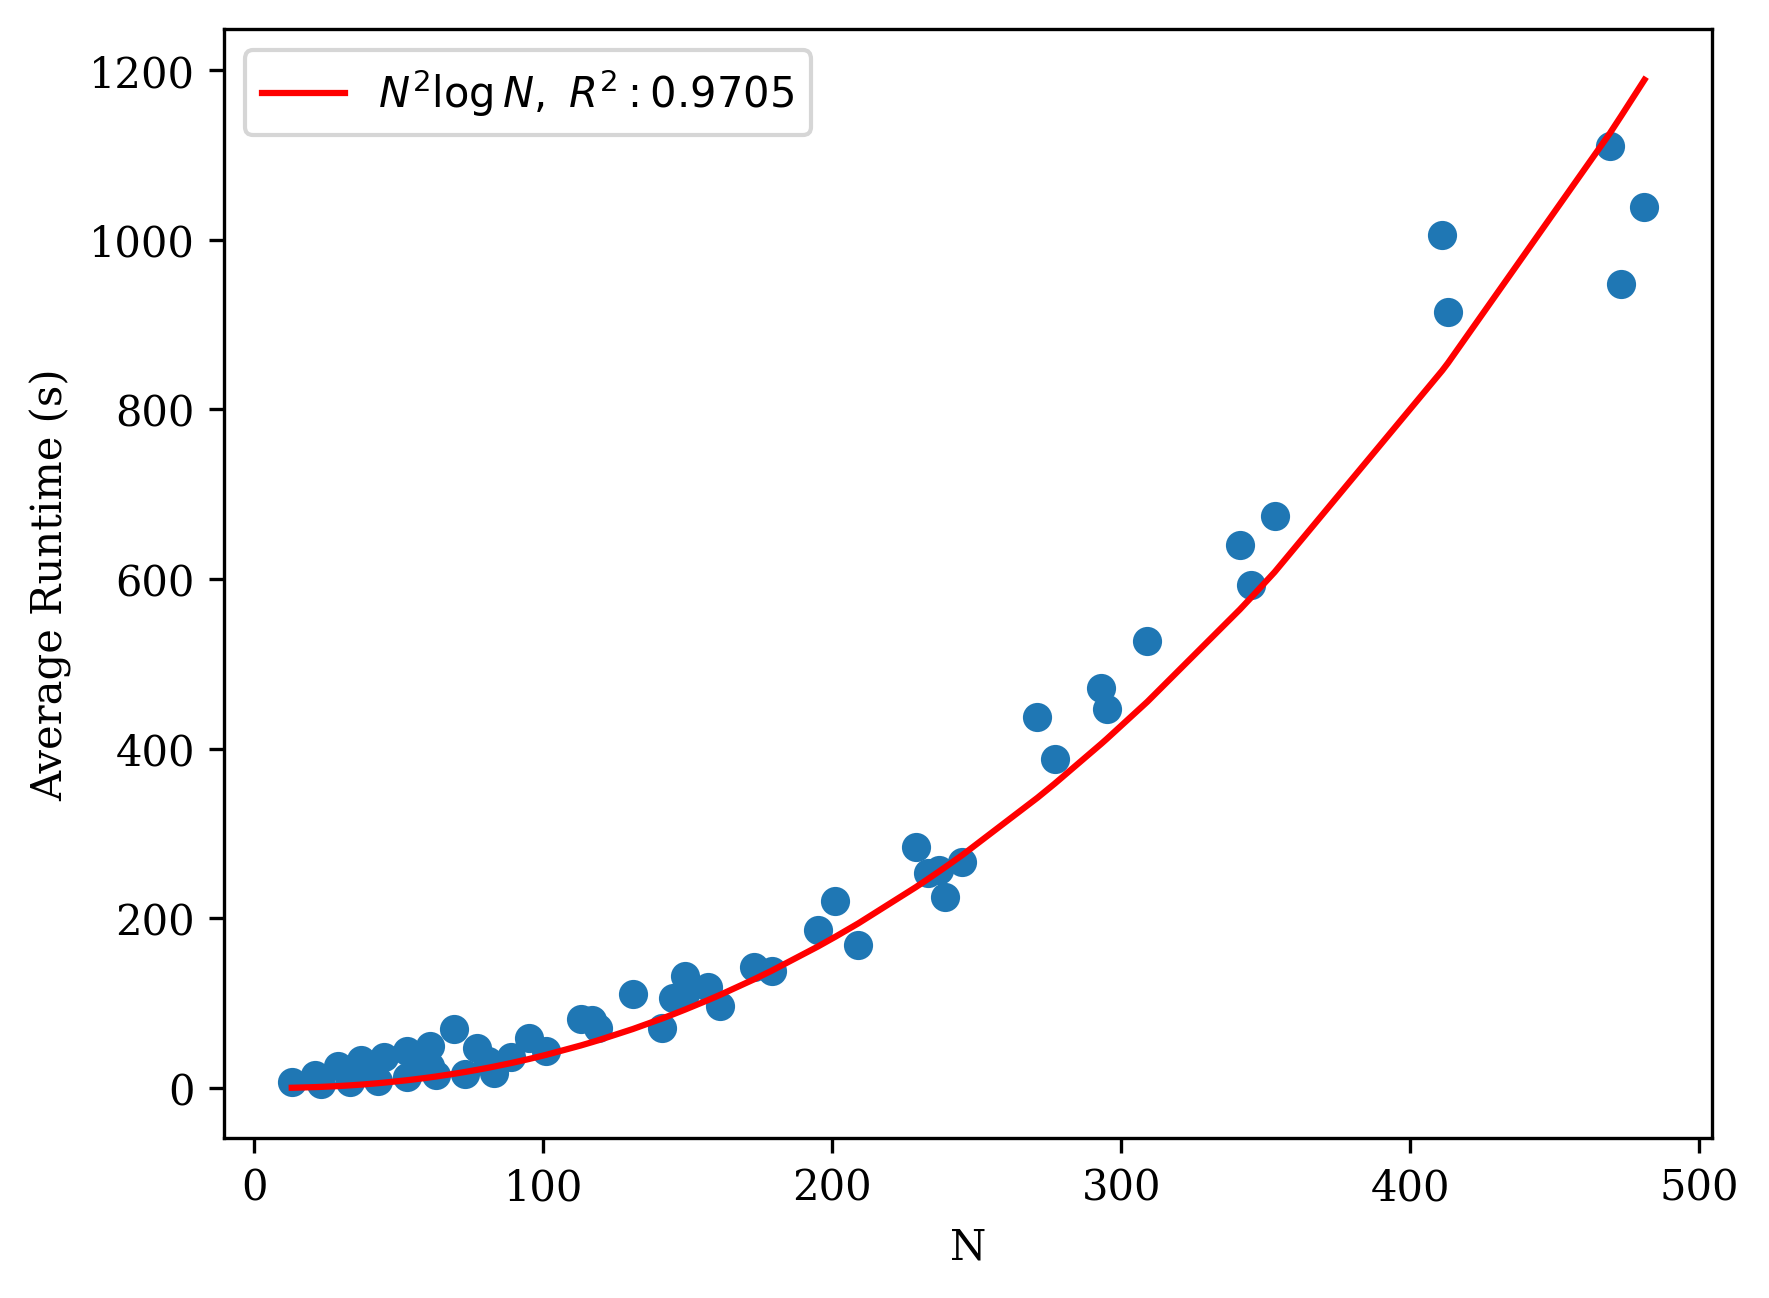
\includegraphics[width=0.8\textwidth]{images/tick-total-runtime.png}
\caption{\label{fig:runtime-tick-aggregate}Average runtime data for running Algorithm \ref{alg:dispatcher-inner}.}
\end{figure}
\section{Architecture}
\label{sec:orgb80524a}

We present a view of the Delay Kirk architecture that focuses attention to its scheduling and
dispatching capabilities. Kirk takes RMPL \citeprocitem{16}{[16]} as input and produces actions as output
(from here on, ``Kirk'' refers to Delay Kirk because the architectural design of Delay Kirk and other
Kirks is fundamentally the same). As shown in Figure \ref{fig:executive-kirk-architecture}, there are
three key components of Kirk.

\begin{figure}[htbp]
\centering
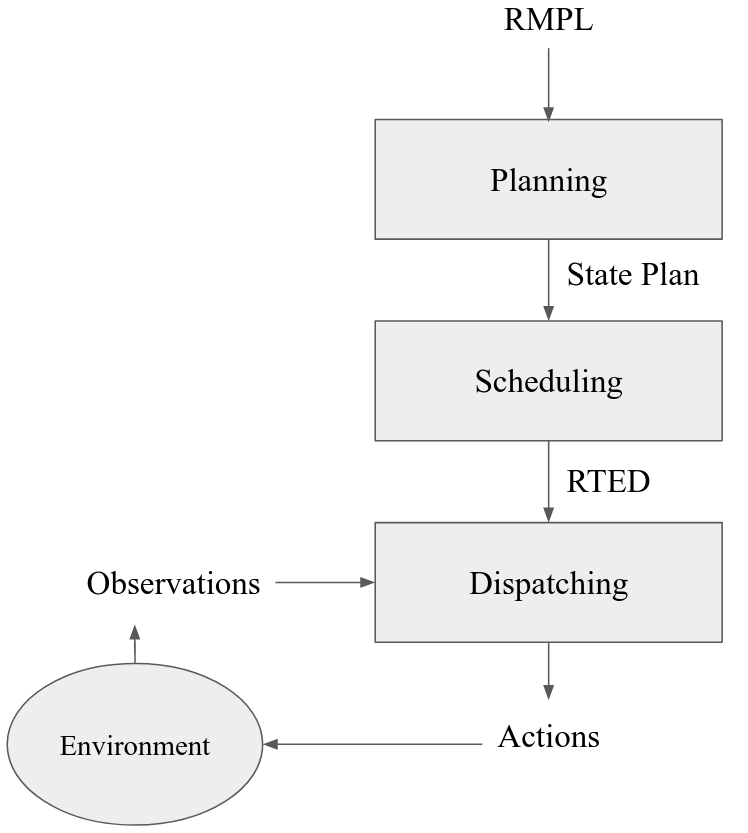
\includegraphics[width=0.6\textwidth]{images/executive-architecture.png}
\caption{\label{fig:executive-kirk-architecture}A simplified, high-level overview of the Delay Kirk task executive architecture with respect to dispatching actions.}
\end{figure}

Figure \ref{fig:executive-kirk-architecture} explicitly identifies the environment. We do so to highlight
that Kirk is designed to be able to interact with the outside world. For instance, if Kirk is
running on a robot, the environment might consist of the pose of the manipulator and any objects in
the scene. If Kirk is responsible for sending notifications to a digital assistant in a spacesuit,
then the environment might be the ``as executed'' version of an EVA timeline. In either case, actions
caused by Kirk will impact the environment. Likewise, Kirk learns from the environment. Here we show
event observations from the environment being sent to the scheduler. However, when Kirk is working
with sub-executives designed for specific problem domains, e.g. risk-bounded motion planning, it may
be monitoring other aspects of the environment as well.

Every Kirk has a planning component that takes RMPL as input, generates state plans, then checks
consistency using OpSAT. OpSAT is similar to a satisfiability (SAT) solver with the property that it
produces optimal assignment to real valued variables. Any temporal constraints in the state plan are
translated to a delay STNU then checked with the variable-delay controllability checker from Chapter
\ref{ch:modeling-tn}.

If the overall state plan is satisfiable, it is then sent to the delay scheduler. Note that earlier
we have said that the delay scheduler takes a temporal network as input. However, Figure
\ref{fig:executive-kirk-architecture} shows a state plan as input to the delay scheduler. Functionally,
there is no difference. There is a one-to-one relationship between state plans and delay STNUs. In
fact, as implemented for this thesis, the delay scheduler can take either a state plan or delay STNU
as input. If a state plan is received, then the first action taken is to convert the state plan to a
delay STNU.

RTEDs that the delay scheduler outputs are sent to a delay dispatcher. As a dispatcher, it has the
primary purpose of translating events to actions that can affect the environment. It is also
responsible for running the loop described in Algorithm \ref{alg:approach-delay-scheduler}. With the
additional requirement of dispatching actions in the presence of observation delay, the delay
dispatcher manages buffered events (see Lemma \ref{lemma:buffering-imagining}) to ensure they are sent to
the delay scheduler at the appropriate time.

\section{RMPL}
\label{sec:org385f457}
\subsection{Constraint Programs}
\label{sec:org566f097}
\label{sec:rmpl}

RMPL is a key component of Kirk. This section steps through example RMPL control programs to
describe their features and our modeling choices. The purpose of this section is three-fold:

\begin{enumerate}
\item A short walkthrough of the language is required in order to explain this thesis' contributions
because an updated RMPL description in any form (e.g. manual, publication, or tutorial) has not
been publicly released since 2003 \citeprocitem{38}{[38]}
\item We must describe the modeling choices of RMPL in sufficient detail to make concrete our approach
to modeling temporal constraints in human-readble form
\item The above is used to demonstrate that modeling uncertain communication delay can be naturally
modeled in RMPL
\end{enumerate}

This section is not meant to be a complete documentation of RMPL, rather our goal is to motivate the
strength of RMPL as a modeling language for human planners describing autonomous systems with
observation uncertainty.

RMPL has undergone a number of rewrites since its inception, and is currently being developed as a
superset of the Common Lisp language using the Metaobject Protocol \citeprocitem{41}{[41]}. The goal is
that a human should have a comfortable means for accurately modeling sufficient detail about the
problem domain such that an executive can perform model-based reasoning to decide how to act.

RMPL and Kirk can be used to achieve a number of different goals. These include but are not limited
to temporal scheduling, classical planning, hybrid planning. For this thesis, we focus on temporal
scheduling and the ability for a human to write \emph{control programs}, or composable constraints and
goals.

For this thesis, we take the assumption that each Kirk executive is responsible for a single agent.
We also ignore vehicle dynamics given this thesis' focus on contributions to temporal scheduling.
However, RMPL is more flexible and allows multi-agent planning and motion planning using vehicle
dynamics, which will be briefly described in Section \ref{sec:rmpl-agents}.

An example of an RMPL control program for a single-agent without agent dynamics follows in Listing
\ref{code:example-control-program}.

\begin{listing}[htbp]
\begin{minted}[]{lisp}
;; NOTE: we omitted Lisp package definitions here for simplicity's sake

(define-control-program eat-breakfast ()
  (declare (primitive)
           (duration (simple :lower-bound 15 :upper-bound 20))))

(define-control-program bike-to-lecture ()
  (declare (primitive)
           (duration (simple :lower-bound 15 :upper-bound 20))))

(define-control-program main ()
  (with-temporal-constraint (simple-temporal :upper-bound 40)
    (sequence (:slack nil)
              (eat-breakfast)
              (bike-to-lecture))))
\end{minted}
\caption{\label{code:example-control-program}A sample control program composed of three constraints. \texttt{eat-breakfast} and \texttt{bike-to-lecture} designate controllable constraints, while the \texttt{main} control program enforces that the constraints are satisfied in series.}
\end{listing}

Looking past the parentheses, we can see different options for defining temporal constraints. For
example, the \texttt{(duration (simple ...))} form is used to define a set-bounded temporal constraint
between a \texttt{:lower-bound} and an \texttt{:upper-bound}. The \texttt{main} control program uses a different form,
\texttt{(with-temporal-constraint ...)} to place an \texttt{:upper-bound} on the overall deadline for scheduling
all events in the control program.

The example control programs in Listing \ref{code:example-control-program} are defined without agents in
that there is an assumption that the Kirk instance that executes this control program must know what
the semantics of \texttt{eat-breakfast} and \texttt{bike-to-lecture} mean and how to execute them.

It could also be the case that Kirk is simply being used to produce a schedule of events offline
that will be handed to an agent that knows how to execute them. As an example, perhaps a student
wants some help planning their morning, so they write an RMPL control program with constraints
representing everything they need to do between waking up and going to lecture, as seen in the more
complex control program in Listing \ref{code:morning-lecture}. The student could ask Kirk to produce a
schedule of events that satisfies all the temporal constraints in this RMPL control program, which
they would then use to plan their morning routine. See the resulting schedule produced by Kirk in
Table \ref{tab:morning-lecture-schedule}. (Note that while normally times in RMPL are represented in
seconds, we use minutes in Listing \ref{code:morning-lecture} and Table \ref{tab:morning-lecture-schedule} for
simplicity's sake.)

\begin{listing}[htbp]
\begin{minted}[linenos,firstnumber=1]{lisp}
;; This file lives in the thesis code repo at:
;;      kirk-v2/examples/morning-lecture/script.rmpl
;;
;; To execute this RMPL control program as-is and generate a schedule, go to the root
;; of the thesis code repo and run the following command:
;;
;; kirk run kirk-v2/examples/morning-lecture/script.rmpl \
;;      -P morning-lecture \
;;      --simulate

(rmpl/lang:defpackage #:morning-lecture)

(in-package #:morning-lecture)

(define-control-program shower ()
  (declare (primitive)
           (duration (simple :lower-bound 5 :upper-bound 10))))

(define-control-program eat-breakfast ()
  (declare (primitive)
           (duration (simple :lower-bound 15 :upper-bound 20))))

(define-control-program review-scheduling-notes ()
  (declare (primitive)
           (duration (simple :lower-bound 10 :upper-bound 15))))

(define-control-program review-planning-notes ()
  (declare (primitive)
           (duration (simple :lower-bound 10 :upper-bound 15))))

(define-control-program pack-bag ()
  (declare (primitive)
           (duration (simple :lower-bound 5 :upper-bound 6))))

(define-control-program bike-to-lecture ()
  (declare (primitive)
           (duration (simple :lower-bound 15 :upper-bound 20))))

(define-control-program review-notes ()
  (sequence (:slack t)
    (review-scheduling-notes)
    (review-planning-notes)))

(define-control-program main ()
  (with-temporal-constraint (simple-temporal :upper-bound 60)
    (sequence (:slack t)
      (shower)
      (parallel (:slack t)
        (eat-breakfast)
        (review-notes))
      (pack-bag)
      (bike-to-lecture))))
\end{minted}
\caption{\label{code:morning-lecture}A student's morning routine preparing for lecture as modeled in RMPL. This is a complete RMPL program that includes the required Lisp package definitions to run in Kirk.}
\end{listing}

\begin{table}[htbp]
\caption{\label{tab:morning-lecture-schedule}The schedule produced by Kirk's scheduler for the student's routine before lecture as modeled in Listing \ref{code:morning-lecture}. Note: Kirk's output has been cleaned for readability purposes.}
\centering
\begin{tabular}{left}
\textbf{Event} & \textbf{Time (min)}\\\empty
\hline
\texttt{START} & 0\\\empty
Start \texttt{shower} & 1\\\empty
End \texttt{shower} & 6\\\empty
Start \texttt{review-scheduling-notes} & 6\\\empty
Start \texttt{eat-breakfast} & 6\\\empty
End \texttt{review-scheduling-notes} & 16\\\empty
Start \texttt{review-planning-notes} & 16\\\empty
End \texttt{eat-breakfast} & 21\\\empty
End \texttt{review-planning-notes} & 26\\\empty
Start \texttt{pack-bag} & 26\\\empty
End \texttt{pack-bag} & 31\\\empty
Start \texttt{bike-to-lecture} & 32\\\empty
End \texttt{bike-to-lecture} & 46\\\empty
\texttt{END} & 46\\\empty
\end{tabular}
\end{table}

Listing \ref{code:morning-lecture} introduces the notion of control programs that are allowed to be
executed simultaneously, as modeled with the \texttt{(parallel ...)} form found in the \texttt{main} control
program on line 48.

Kirk is able to simulate the RMPL script in Listing \ref{code:morning-lecture} and produce a schedule
because there were no uncontrollable constraints, that is, all control programs are under the
agent's control. Say we replaced \texttt{bike-to-lecture} with \texttt{drive-to-lecture}. Due to traffic
conditions, driving presents in an uncontrollable constraint. RMPL allows us to model uncontrollable
constraints as in Listing \ref{code:drive-to-lecture}.

\begin{listing}[htbp]
\begin{minted}[]{lisp}
(define-control-program drive-to-lecture ()
  (declare (primitive)
           (duration (simple :lower-bound 15 :upper-bound 20)
                     :contingent t)))
\end{minted}
\caption{\label{code:drive-to-lecture}An uncontrollable, or contingent, temporal constraint in a control program.}
\end{listing}

The addition of \texttt{:contingent t} to the \texttt{(duration ...)} form tells Kirk that it does not have
control over when the end of \texttt{drive-to-lecture} is scheduled, rather, Nature (i.e. traffic
conditions) chooses a time. Despite the lack of control over \texttt{drive-to-lecture}, we do know the
drive should take between 15 and 20 minutes, hence our model includes \texttt{:lower-bound 15} and
\texttt{:upper-bound 20}.

With uncontrollable constraints in a control program, we are no longer guaranteed to be able to
produce a schedule offline as we show in Table \ref{tab:morning-lecture-schedule}. Instead, as time
passes, we may only choose to schedule controllable events based on the \emph{partial history} of
contingent event assignments so far, or, in other words, perform \emph{dynamic scheduling}. Thus, we can
no longer simulate a schedule with Kirk. We must connect Kirk to a source for receiving contingent
event assignments in order to make valid controllable event assignments. Our approach to dynamic
scheduling is the focus of Chapter \ref{ch:delay-scheduling}.

As a contribution of this thesis, our existing approach to specifying durations in RMPL was expanded
to model observation delay. An example follows in Listing \ref{code:rmpl-obs-delay} modeling a sample
collection control program with observation delay.

\begin{listing}[htbp]
\begin{minted}[]{lisp}
(define-control-program collect-science-sample ()
  (declare (primitive)
           (duration (simple :lower-bound 15 :upper-bound 30
                             :min-observation-delay 5
                             :max-observation-delay 15)
                     :contingent t)))
\end{minted}
\caption{\label{code:rmpl-obs-delay}An RMPL control program describing a science data collection task with observation delay.}
\end{listing}

We can see in Listing \ref{code:rmpl-obs-delay} that representing set-bounded observation delay is a
simple as adding \texttt{:min-} and \texttt{:max-observation-delay} to the \texttt{(duration (simple ...) :contingent t)}
form. In full, this control program represents an uncontrollable constraint with a contingent event
that Nature will schedule \([15, 30]\) time units after sample collection begins. The executive will
then wait an additional \([5, 15]\) time units before learning that \texttt{collect-science-sample} has been
scheduled. As will be described in much greater detail in Section \ref{sec:vdc}, the executive will only
learn \emph{that} the contingent event occurred - is not guaranteed to learn where in \([15, 30]\) the
contingent event was assigned, nor will it know how much observation delay was incurred.


\subsection{Action Model}
\label{sec:org2b2ed16}
\label{sec:rmpl-agents}

This section is included to expand on the features of RMPL, though note that none of these features
are required for controlling distributed agents, and were not a part of the experiments for this
research.

If we wanted to specify agents in a multi-agent control program, or if we wanted to take vehicle
dynamics into account, RMPL gives us a means for using the Common Lisp Object System (CLOS) for
defining agents, agent dynamics, and the control programs agents may execute.

An example RMPL control program with an agent is provided in Listing \ref{code:glider-simple} for
completeness sake from the domain of underwater robotics.

\begin{listing}[htbp]
\begin{minted}[]{lisp}
;; This code is a snippet from a file in the thesis code repo found at:
;;      kirk-v2/examples/glider/script.rmpl

(defclass glider ()
  ((id
    :initarg :id
    :finalp t
    :type integer
    :reader id
    :documentation
    "The ID of this glider.")
   (deployed-p
    :initform nil
    :type boolean
    :accessor deployed-p
    :documentaiton
    "A boolean stating if the glider is deployed at any point in time.")
   (destination
    :initform nil
    :type (member nil "start" "end" "science-1" "science-2")
    :accessor destination
    :documentation
    "The location to which the glider is currently heading, or NIL if it is not
    in transit.")
   (location
    :initarg :location
    :initform "start"
    :type (member nil "start" "end" "science-1" "science-2")
    :accessor location
    :documentation
    "The location where the glider is currently located, or NIL if it is not at
    a location (in transit).")))

(define-control-program move (glider to)
  (declare (primitive)
           (requires (and
                      (over :all (= (destination glider) to))))
           (effect (and
                    (at :start (= (destination glider) to))
                    (at :start (= (location glider) nil))
                    (at :end (= (destination glider) nil))
                    (at :end (= (location glider) to))))
           (duration (simple :lower-bound 10 :upper-bound 20))))
\end{minted}
\caption{\label{code:glider-simple}A snippet of an RMPL script that defines an agent and classical planning predicates and effects of a control program.}
\end{listing}

In Listing \ref{code:glider-simple}, \texttt{glider} refers to a low-powered autonomous underwater vehicle that
prefers to traverse by following ocean currents using a buoyancy engine.\footnote{The Slocum Glider is
an example: \href{https://www.whoi.edu/what-we-do/explore/underwater-vehicles/auvs/slocum-glider/}{https://www.whoi.edu/what-we-do/explore/underwater-vehicles/auvs/slocum-glider/.}} We see
that we model a \texttt{glider} agent and its properties using standard CLOS. The \texttt{move} control program
then takes a \texttt{glider} and a \texttt{location} as arguments. The \texttt{(requires ...)} form is equivalent to the
preconditions of a durative action in a PDDL 2.1 \citeprocitem{42}{[42]} domain. Likewise, the \texttt{(effect
...)} form is equivalent to PDDL effects. Finally, as we saw before, the durative action also
includes a temporal constraint in its \texttt{(duration ...)} form.

Kirk is able to take RMPL as input to perform classical planning, though further discussion of it
falls outside the scope of this thesis.

\chapter{Coordinating Multiple Agents under Uncertain Communication}
\label{sec:org6748992}
\label{ch:technical-coordination}

In this chapter, we present a novel MA framework for dynamic event scheduling with inter-agent
temporal constraints. Our framework adheres to the variable observation delay modeling framework
presented in Chapter \ref{ch:modeling-tn}, making it robust to uncertain communication.

Online MA coordination of event dispatching allows executives to dynamically decide when to act
given the resolution of inter- and intra-agent temporal constraints. In our formulation, each
executive has its own STNU with contingent events it expects to observe and free events it is
responsible for monitoring. We do not distinguish between contingent events that are the free events
scheduled by peer agents and contingent events from any other source in Nature. There are no
restrictions on inter-agent constraints, though they must avoid chained contingencies the same way
that vanilla, single-agent STNUs do \citeprocitem{27}{[27]}.


Executives are \emph{not} required to have perfect knowledge of the complete state of the world with
respect to event assignments, nor are they required to even \emph{agree} on the state of the world.
Rather, their knowledge should be consistent with the temporal constraints and observation delay
modeled in their individual delay STNUs. This requirement stands in opposition to the communication
challenge that is commonly addressed in problems involving distributed agents, e.g. distributed
consensus approaches \citeprocitem{43}{[43]}, \citeprocitem{44}{[44]}, where it is crucial that all agents agree on
the state of the world. In our framework, each agent acts according to their given constraints. Due
to scheduling uncertainty from observation delay, it is impossible to expect agents to agree on
partial histories, nor is it necessary because each agent is capable of scheduling events with
observation uncertainty.

To our knowledge, no such online scheduler for MA coordination with this requirement has been
proposed. In this chapter, we first present a grounded Artemis-like scenario to motivate
coordination. Next, we describe a modeling framework for MA control programs that is necessary for
establishing coordination between agents. Then we define an event propagation algorithm used to
guarantee that event observations match individual agent STNUs. We finish by presenting experimental
analysis of our event propagation algorithms, and the results of hardware demonstrations of Delay
Kirk using a robotic arm and a simulated astronaut.

\section{Multi-Agent Control Programs}
\label{sec:orgdcb8900}
\label{sec:ma-control-programs}

This thesis introduces challenges in writing control programs for multiple agents who need to
coordinate. We do not claim to solve all aspects of coordination, rather we present a framework for
simple scenarios with the key feature being that agents need to agree on the \emph{order} of a subset of
events. We start by presenting an example of inter-agent temporal constraints, followed by defining
a modeling technique for guaranteeing that agents agree about the order of events in their
respective partial histories. To the best of our knowledge, we are unaware of any other MA framework
for coordinating the order of event histories.

Consider two agents, \texttt{agent1} and \texttt{agent2}, that are scheduling STNUs \(S_{1}\) and \(S_{2}\)
respectively. \(S_{1}\) and \(S_{2}\) share a subset of semantically similar episodes, \(e_{1}\) and
\(e_{2}\). \texttt{agent1} ``owns'' \(e_{1}\), meaning it is responsible for scheduling the free event
\(e_{1}\)​-start and observing the contingent event \(e_{1}\)​-end, while \texttt{agent2} owns \(e_{2}\). It is the
case that \(e_{1}\) must precede \(e_{2}\) in \(S_{1}\) and \(S_{2}\). A simplified MA view of the
constraints is as follows.

$$
\conedge{e_{1}\text{-start}}{e_{1}\text{-end}}{[15, 30]}
\edge{}{e_{2}\text{-start}}{[0, \infty]}
\conedge{}{e_{2}\text{-end}}{[22, 26]}
$$

From \texttt{agent1}'s perspective, \(S_{1}\) models the following constraints. We add a \texttt{noop} start event,
\(Z\), to simplify coordination. For now, we allow chained contingencies, though in a moment they will
need to be addressed.

$$
\edge{Z}{e_{1}\text{-start}}{[0, 0]}
\conedge{}{e_{1}\text{-end}}{[15, 30]}
\conedge{}{e_{2}\text{-start}}{[0, \infty]}
\conedge{}{e_{2}\text{-end}}{[22, 26]}
$$

We assume that \texttt{agent1} models \(e_{2}\) in \(S_{1}\) because other events under their control depend on
\(e_{2}\). \(S_{2}\) is then modeled as follows. Note the change to the controllability of
\(\conedge{Z}{e_{1}\text{-start}}{[0, 0]}\).

$$
\conedge{Z}{e_{1}\text{-start}}{[0, 0]}
\conedge{}{e_{1}\text{-end}}{[15, 30]}
\edge{}{e_{2}\text{-start}}{[0, \infty]}
\conedge{}{e_{2}\text{-end}}{[22, 26]}
$$

For the sake of controllability of \(S_{1}\) and \(S_{2}\), we would simply add \([0, 0]\) free
constraints between consecutive contingent constraints. Also note that from a scheduling standpoint,
there is no difference between \(\edge{a}{b}{[0, 0]}\) and \(\conedge{a}{b}{[0, 0]}\) - both indicate
\(a\) and \(b\) should be scheduled simultaneously.

We will walk through scheduling this scenario from the perspective of both agents. First, we
describe their actions in the case that there is no communication delay, then we introduce
communication, and finally we add delay to communications. This scenario will motivate our analysis
of the challenges that arise in MA control programs.

If both agents have perfect knowledge of the world (instantaneous knowledge of events), scheduling
is trivial. \texttt{agent1} and \texttt{agent2} execute \(Z\) simultaneously. \texttt{agent1} schedules \(e_{1}\)​-start and
\texttt{agent2} instantaneously receives an observation of \(e_{1}\)​-start. \(e_{1}\)​-end arrives in \([15, 30]\)
later, which again, both agents observe simultaneously. Now \texttt{agent2} is free to act. It schedules
\(e_{2}\)​-start, which \texttt{agent1} observes instantaneously. \(e_{2}\)​-end arrives \([22, 26]\) later and is
observed simultaneously by both agents.

Now, we enforce that \texttt{agent1} ``owns'' \(e_{1}\) and is the only agent that can observe it directly.
Likewise, \texttt{agent2} owns \(e_{2}\). In order for an agent to learn about an episode they do not own,
they must receive a communication from the agent who does. After \texttt{agent1} schedules \(e_{1}\)​-start,
it must send a message to \texttt{agent2}. \texttt{agent2} receives said message, which it interprets as an
observation of \(e_{1}\)​-start. If communications are instantaneous, the partial histories of both
agents agree on the assignment of \(e_{1}\)​-start. Later \(e_{1}\)​-end is observed by \texttt{agent1}, who is
then responsible for relaying a communication to \texttt{agent2} indicating that it is safe to assign
\(e_{1}\)​-end. \texttt{agent2} is now free to schedule \(e_{2}\)​-start, which it does instantaneously. The same
pattern of sending messages that events have been scheduled repeats and \texttt{agent1} learns that
\(e_{2}\)​-start was schedule simultaneously with \(e_{1}\)​-end. After all events have been scheduled,
the histories of \texttt{agent1} and \texttt{agent2} still agree on the times assigned to each event.

We now show that adding delay to the communications between agents forces us to add
\emph{synchronization} episodes to \(S_{1}\) and \(S_{2}\) to maintain event ownership. First, we must
address the chained contingencies. Note that we have freedom in how we model the constraints of this
scenario. The following example will motivate the need for a synchronization episode while remaining
as close to the semantics of the original STNU as possible.

From the perspective of \texttt{agent1}, \(S_{1}\), we cannot escape the fact that there are two
uncontrollable events in sequence - the end of \(e_{1}\) and the start of \(e_{2}\), if we try to
separate the events with a synthetic requirement episode, \(\sigma\), with a \([0, \infty]\) constraint,
the semantics no longer respect the original scenario.

$$
\edge{Z}{e_{1}\text{-start}}{[0, 0]}
\conedge{}{e_{1}\text{-end}}{[15, 30]}
\edge{}{\sigma\text{-start}}{[0, 0]}
\edge{}{\sigma\text{-end}}{[0, \infty]}
\conedge{}{e_{2}\text{-start}}{[0, 0]}
\conedge{}{e_{2}\text{-end}}{[22, 26]}
$$

The delay scheduler will choose to schedule \(\sigma\)​-end simultaneously with \(\sigma\)​-start, also
leading to \(e_{2}\)​-start being immediately scheduled. However, \(e_{2}\) is not under \texttt{agent1}'s
control, and thus it has no authority to schedule \(e_{2}\)​-start. Instead, our synthetic constraint
also needs to be contingent.

$$
\edge{Z}{e_{1}\text{-start}}{[0, 0]}
\conedge{}{e_{1}\text{-end}}{[15, 30]}
\edge{}{\sigma\text{-start}}{[0, 0]}
\conedge{}{\sigma\text{-end}}{[0, \infty]}
\edge{}{e_{2}\text{-start}}{[0, 0]}
\conedge{}{e_{2}\text{-end}}{[22, 26]}
$$

Now, the issue is that \(S_{1}\) is uncontrollable due to
\(\conedge{\sigma\texttt{-start}}{\sigma\texttt{-end}}{[0, \infty]}\). We know the \texttt{agent2} will
receive \(e_{1}\)​-end somewhere in \(\gammabar'(e_{1}\texttt{-end})\), where the \(\gammabar'\) function
represents observation delay in \(S_{2}\). \texttt{agent2} will then immediately schedule \(e_{2}\)​-start.
Finally, \(S_{1}\) becomes

$$
\edge{Z}{e_{1}\text{-start}}{[0, 0]}
\conedge{}{e_{1}\text{-end}}{[15, 30]}
\edge{}{\sigma\text{-start}}{[0, 0]}
\conedge{}{\sigma\text{-end}}{[\gammabar'^-(e_{1}\texttt{-start}), \gammabar'^-(e_{1}\texttt{-end})]}
\edge{}{e_{2}\text{-start}}{[0, 0]}
\conedge{}{e_{2}\text{-end}}{[22, 26]}
$$

In practice, an agent may choose to schedule other events while waiting for \(\sigma\)​-end to arrive.

In \(S_{2}\), we may choose to give \texttt{agent2} the same synchronization episode without changing the
execution semantics. We know that \(e_{1}\)​-end will be observed somewhere in
\(\gammabar'(e_{1}\texttt{-end})\). When \(e_{1}\)​-end arrives, we are guaranteed to have waited
somewhere in the lower and upper bounds \(\sigma\). Assuming \texttt{agent2} knows that \(e_{1}\)​-end and
\(\sigma\)​-end semantically represent the same point in time, \(\sigma\)​-end can be safely scheduled as
soon as \(e_{1}\)​-end arrives.

Synchronization episodes allow inter-agent constraints with observation delay to be modeled without
impacting the ordering of events. They are used to separate control programs in the hardware
demonstration in Section \ref{sec:hw-demo}.

\section{Event Propagation}
\label{sec:org9e41c60}
\label{sec:event-propagation}

At a high level, scheduled events propagate through a simple directed graph of connected executives.
We put checks in place to ensure that cycles do not cause infinitely recursed event observations.

\begin{defn}
\label{def:communication-graph}
\textbf{Communication Graph}

A \emph{communication graph} \(C\) is a tuple \(\langle V, E \rangle\), where:
\begin{itemize}
\item \(V\) is a set of vertices representing peer executives,
\item \(E\) is a set of directed edges between \(v \in V\) representing the path of event observation
propagation,
\item Each edge \(e_{i} \in E\) is a pair \((o, t)\), where \(o, t \in V\) represent the origin and
termination of the edge respectively.
\end{itemize}

Self-loops, or self-edges, are not allowed, i.e. for any vertex \(v_{i} \in V\), no single edge \(e_{i}
\in E\) may both originate and terminate at \(v_{i}\).
\end{defn}

For some executive \(v_{i} \in V\) with outgoing edges in \(E\), \((v_{i}, v_{j})\), \(\cdots\), \((v_{i},
v_{k})\), any scheduled events that \(v_{i}\) assigns, whether free or contingent, are propagated to
all peer executives \(v_{j}\), \(\cdots\), \(v_{k}\). Likewise, all contingent events received from Nature
are propagated to peers. Finally, any events \(v_{i}\) receives from other agents are also relayed to
peers.

\begin{defn}
\label{def:event-propagations}
\textbf{Event Propagation Messages}

An \emph{event propagation message} \(m\) is a tuple \(\langle x, P \rangle\), where:
\begin{itemize}
\item \(x\) is a set of one or more events scheduled simultaneously,
\item \(P \subseteq V\) is a set of executives who have already received the message.
\end{itemize}
\end{defn}

Recognize that Definition \ref{def:event-propagations} is vague in defining \(x\). Event propagation
messages are passed between agents, and each agent has its own STNU. In some cases, \(x\) will be free
events, in others \(x\) will be contingent events. The type of event makes no difference to the
algorithm so we do not distinguish between them here.

Events that are received in \(m\), \(m[x]\), are handled the same as observations of contingent events
during scheduling. Lemmas \ref{lemma:information-fixes-bounds}, \ref{lemma:ignore-inf-delay}, and
\ref{lemma:subtract-gamma} are applied as appropriate when the observation of \(m[x]\) arrives.

For an edge \((v_{i}, v_{j}) \in E\), it is possible that \(v_{j}\) receives events that are not present
in its STNU.

Because we have not defined a temporal decoupling-like algorithm wherein an STNU for multiple-agents
is programmatically separated into individual STNUs (see the discussion of multi-agent STNUs
\citeprocitem{11}{[11]} in Section \ref{sec:mastnus}), we are reliant on human planners to write STNUs for
each agent by hand. As a result, there is no guarantee that \(x\) is meaningful to a given agent.

To be more specific, there is no guarantee that any event \(x_{i} \in x\) in the event propagation
message has an equivalent event in \(X_{c}\) of the STNU being executed by any receiving agent \(v_{j}
\in V\). If agent \(v_{j}\) cannot find \(x_{i}\) in their \(X_{c}\), then \(x_{i}\) can be ignored. As will
be discussed in Algorithm \ref{alg:event-propagation}, we represent \(x\) using a type that can be compared
for equivalence with the events in an agent's STNUs, e.g. a list of strings.

We use \(P\) to avoid cycles in event propagation. As will be shown in Algorithm
\ref{alg:event-propagation}, agent \(v_{i}\) will avoid propagating \(x\) to any agents in \(P\). Agent \(v_{i}\)
will also grow \(P\) when it relays \(m\) to other agents by appending to \(P\) itself and all outgoing
agents \(v_{j}, \cdots, v_{k}\).

Timing information, e.g. timestamps, is explicitly excluded from \(m\). Dynamic scheduling and the
variable-delay STNU and event observation, \(\obs\), formalisms do not account for timestamps.
Instead, we expect that passing messages for event propagation between executives takes an amount of
time in the domain \(\mathbb{R^{+}}\). Thus, when \(v_{j}\) expects to receives an event, \(x_{i} \in x\),
from \(v_{i}\), the time delay can be naturally modeled in the variable-delay function,
\(\gammabar({x_{i}})\), in the STNU that \(v_{j}\) will execute.

If event propagation messages were to include accurate timestamps, we would need to modify the way
events are recorded during scheduling, impacting scheduling Lemmas \ref{lemma:information-fixes-bounds},
\ref{lemma:ignore-inf-delay}, and \ref{lemma:subtract-gamma}. Scheduling events in the past could also impact
controllability. For these reasons, we avoid the inclusion of timestamps in event propagation
messages.

By Definition \ref{def:event-propagations}, events received from other agents are no different than events
received from Nature, and no special considerations are required for scheduling.

We now walk through the process of passing messages between agents as shown in Algorithm
\ref{alg:event-propagation}. We use the same \emph{Event Propagation} algorithm in three cases:

\begin{enumerate}
\item When an agent \(v_{i}\) schedules free events \(x\),
\item When \(v_{i}\) receives an observation from Nature of contingent events \(x\),
\item When \(v_{i}\) receives an incoming message \(m_{i}\) with contingent events \(m_{i}[x]\) from another
agent in \(V\).
\end{enumerate}

Let \texttt{peers} be a mutable set initialized to the terminal vertices for all \(e \in E\) originating at
\(v_{i}\).

In the first case, agent \(v_{i}\) fulfills its responsibilities as defined in \(C\) by broadcasting \(x\)
to its \texttt{peers}, who will receive \(x\) as exogenous contingent events. The outgoing message \(m_{o}\)
that will be passed to \texttt{peers} will include enough information such that no agent should receive a
given \(x\) more than once. To do so, we let \(P\) be a set of all agents that will have observed \(x\)
when \(m_{o}\) is received by \texttt{peers}, \(P = \{ v_{i}, p~ \forall~ p \in \texttt{peers} \}\). We
finalize \(m_{o} = \langle x, P \rangle\), which we simultaneously transmit to each \(p\) in \texttt{peers}.
Transmission is a ``fire and forget'' operation, where \(v_{i}\) does not wait for acknowledgment from
any \(p\) that \(m_{o}\) was received.

The second case plays out the same as the first, the only difference being that \(x\) is itself
observed from Nature. Once again, we let \(P\) be a list of \(v_{i}\) and all \texttt{peers}, and then transmit
\(m_{o}\) simultaneously to all \texttt{peers}.

The third case is a relay operation. Agent \(v_{i}\) is responsible for propagating events \(m_{i}[x]\)
that it has just observed, but we want to avoid sending the events to \texttt{peers} who have already
observed them. We remove those agents from \texttt{peers} accordingly with a set difference operation:
\texttt{peers} \(= \texttt{peers} - m_{i}[P]\). Likewise, we grow the list of agents who have received \(x\),
which is now \(P = P \cup \texttt{peers}\). Agent \(v_{i}\) composes a new \(m_{o} = \langle m_{i}[x], P
\rangle\) and transmits it to \texttt{peers}.

Ideally, the Event Propagation algorithm should run on a separate thread from the main scheduling
loop, else we run the risk of incurring unnecessary delays in observing and dispatching events.

\begin{algorithm}
\SetAlgoLined
\SetKwComment{Comment}{/*}{*/}
\SetKwFunction{Return}{return}
\SetKwInput{Input}{Input}
\SetKwInput{Algorithm}{\textsc{Event Propagation}}
\SetKwInput{Initialize}{Initialization}
\SetKwIF{If}{ElseIf}{Else}{if}{then}{else if}{else}{endif}

\Indm
\Input{Incoming message $m_{i}$; Scheduled events $x$; Self $v_{i} \in V$; Set of outgoing $\texttt{peers} \subset V$}

\Indp
\Algorithm{}
\Indp

$\texttt{peers} \gets \texttt{peers} - m_{i}[P]$\;

$P \gets m_{i}[P] \cup \{ v_{i} \} \cup \texttt{peers}$\;

$x \gets x$ or $m_{i}[x]$\;

$m_{o} \gets \langle x, P \rangle$\;

\For{each $p$ in $\texttt{peers}$} {
    Perform a non-blocking transmission of $m_{o}$ to $p$\;
}

\caption{An event propagation algorithm that avoids recursive message passing.}
\label{alg:event-propagation}
\end{algorithm}

The complexity of Algorithm \ref{alg:event-propagation} is trivially \(O(N)\), where \(N\) is the number of
executives in \(V - 1\). The limiting factor to the performance of Event Propagation will be the time
it takes to transmit messages between agents, which, to reiterate, should be modeled in the delay
functions for any inter-agent temporal constraints.

\section{Experimental Analysis}
\label{sec:org2a79a4f}
\label{sec:ma-experimental}

We performed two demonstrations of the Event Propagation algorithm. The first was a hardware
demonstration performed on a Barrett WAM manipulator in the MERS lab. The second is a multi-agent
simulation showcasing inter-agent constraints. Both will be described below.

\subsection{Distributed Kirk Simulation}
\label{sec:org66dcae9}
\label{sec:dkirk-simulation}

To demonstrate multi-agent communication, we built a simulation of an end-to-end mission with three
independent Kirks, \texttt{agent0}, \texttt{agent1}, and \texttt{agent2}. We will show that distributed Kirks can
successfully dispatch events within temporal bounds in the face of multiple sources of communication
uncertainty. The Kirks are responsible for executing an installation procedure with the same
randomly generated constraints as used in the validation of the delay scheduler in Section
\ref{sec:scheduling-experimental}. In this scenario, each agent is responsible for installing two
satellite dishes with staggered confirmations so as to limit uplink bandwidth usage. As Kirks
receive confirmation that installation has been completed, they then share the confirmations with
their peers.

To simplify comparing schedules, we used a standardized format for event names. Repeated event names
are given as \texttt{Event:[agent]:[iteration]}, where \texttt{[agent]} and \texttt{[iteration]} are zero-indexed. For
instance, \texttt{Install:4:3} would be the start of an installation episode for a hypothetical \texttt{agent4}
(of at least five agents) in its fourth iteration.

There is one modification from the original constraints from Section \ref{sec:scheduling-experimental} in
that we separate the communication delay inherent to the confirmation task with the observation
delay inherent to sharing observations with peers. There may be a delay waiting for confirmation
from ground, and the \emph{in situ} communication infrastructure may add an additional delay to
communications between agents. We assume the sources of delay compound. For instance, \texttt{agent1} will
need to know when \texttt{agent0} has confirmed its installation task, \texttt{Confirm:0:0} before beginning their
own installation, \texttt{Install:1:0}. if \texttt{agent0} expects to receive \texttt{Confirm:0:0} with an observation
delay of \(\gammabar(\texttt{Confirm:0:0}) = [0, 10]\), we increase
\(\gammabar^+(\texttt{Confirm:0:0})\) by one for any peers that receive the observation broadcasted
from \texttt{agent0}. In other words, from the perspective of \texttt{agent1} or \texttt{agent2},
\(\gammabar(\texttt{Confirm:0:0}) = [0, 11]\) instead.

\begin{figure}[htbp]
\centering
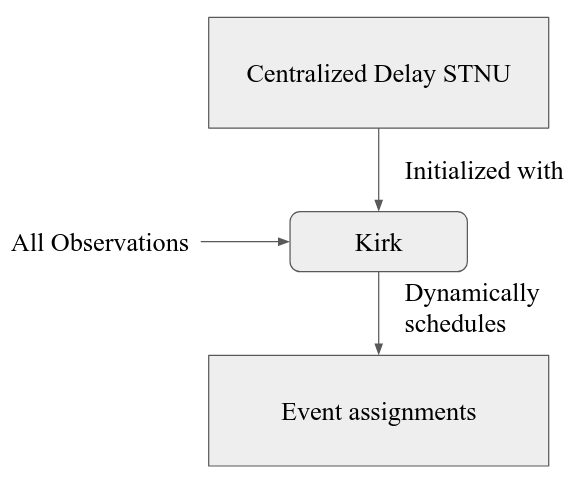
\includegraphics[width=3in]{images/demo-centralized.png}
\caption{\label{fig:demo-centralized}The Kirk architecture used to generate event assignments for the centralized delay STNU. A single Kirk receives the VDC STNU that includes constraints for all agents, as well as contingent event observations. Kirk then performs delay scheduling, resulting in an assignment to all events.}
\end{figure}

At a high-level, our procedure for creating this demonstration is as follows. We randomly generated
a variable-delay STNU for three agents and two installation procedures (using the same generator
code that was used in Section \ref{sec:scheduling-experimental}) and confirmed it to be VDC. We call this
STNU the \emph{centralized delay STNU} in that it includes all constraints for all three agents in a
multi-agent mission with observation delay. We then acted like a mission planner in that we manually
decoupled the centralized delay STNU into three single-agent RMPL control programs. Each control
program contained the subset of the constraints from the centralized delay STNU required for a
single agent to maintain the semantics of the original constraints. We call the variable-delay STNUs
represented by the collection of the three RMPL control programs the \emph{distributed variable-delay
STNUs}. We finally pre-determined when observations would arrive for each agent to simplify running
the demonstration. Both the centralized and distributed scenarios received observations of the same
events at the same times.

The architecture for the centralized scenario is shown in Figure \ref{fig:demo-centralized}, while the
distributed scenario is represented in Figure \ref{fig:demo-distributed}. Figure \ref{fig:demo-distributed}
presents a simplified view in order to keep the diagram readable. In reality, each Kirk broadcasts
all events to all peers.

\begin{figure}[htbp]
\centering
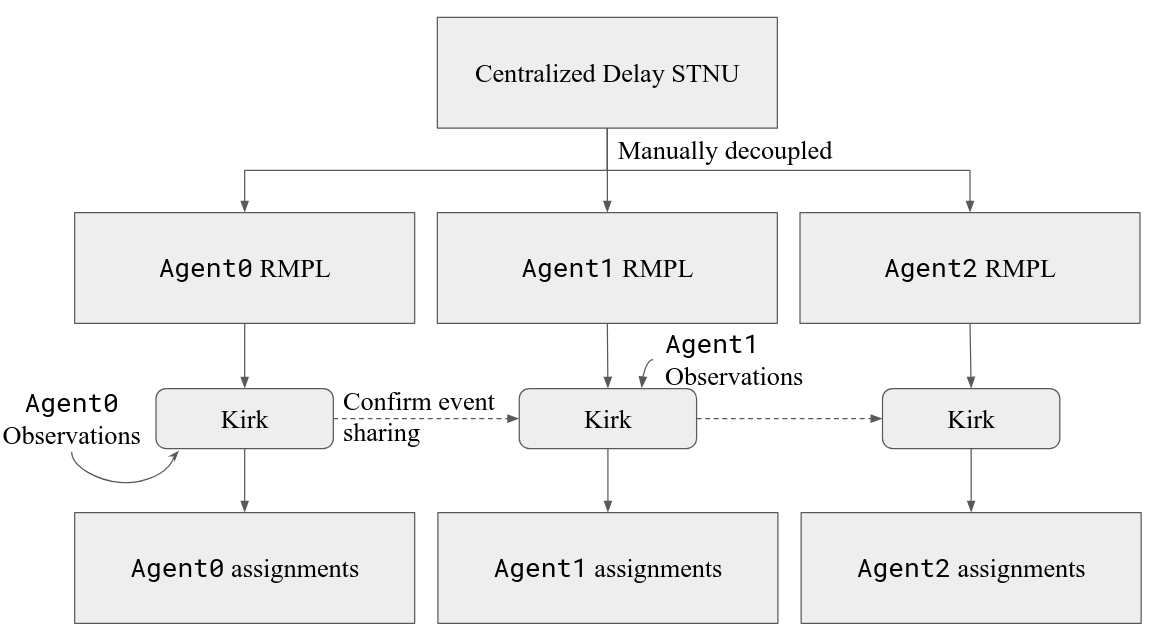
\includegraphics[width=\textwidth]{images/demo-distributed.png}
\caption{\label{fig:demo-distributed}The distributed architecture for the demonstration. The original centralized delay STNU is manually decoupled to three separate RMPL control programs, which are then used to initialize three Kirks. The Kirks receive appropriate event observations, which they then share to their peers. After delay scheduling, each Kirk produces an assignment to events that were under their control.}
\end{figure}

Event observations were arranged as follows. In the centralized case, the single Kirk received all
contingent event observations. Any observations that were not explicitly provided as an observation
was assumed to be assigned at its upper bound. In the distributed case, Kirks were only given event
observations for events that belong to them. For instance, only \texttt{agent0} received an observation of
\texttt{Confirm:0:0}, the event signifying that they have completed installation of the first satellite. It
was then the responsibility of \texttt{agent0} to broadcast the event observation to its peers.

To evaluate the ability of a distributed Kirk architecture to perform scheduling with communication
uncertainty, we focus on the schedules produced. To do so, we compare the schedule created by a Kirk
running against centralized delay STNU (Table \ref{table:centralized-schedule}) against the combined schedules
of the three single agents (Tables \ref{table:agent0-schedule}-\ref{table:agent2-schedule}). If observations
arrive at the same time, both scenarios should yield the same schedules. Importantly, the
inter-agent constraint between overlapping installation tasks should hold in the distributed
scenario. The confirmation events are highlighted in gray in each table for ease of identification.

Running the demonstration was then a matter of running three networked instances of Kirk
simultaneously against three different control programs. We did so using a \texttt{Makefile} with three
targets, running \texttt{make} with the \texttt{-j3} flag, and setting up communications to take place over HTTP.

From the root of the thesis repository, execute \texttt{make kirk \&\& make -j3 demo} to run the
demonstration. The resulting schedules will be written to \texttt{agent\{0,1,2\}.txt}. Note that the STNU was
generated directly for the centralized delay STNU, but the STNUs were compiled from RMPL control
programs for the distributed delay STNUs. There are naming differences between the events of the
different schedules due to way control programs receive names in RMPL and the way RMPL control
programs are compiled to STNUs. The event names in schedules in Tables
\ref{table:centralized-schedule}-\ref{table:agent2-schedule} have been manually altered such that they match here.
See Appendix \ref{appendix:rmpl} for a description of the resulting STNUs from RMPL control programs.

\begin{table}[htbp]
\caption{\label{table:centralized-schedule}The schedule produced by a single Kirk against against the ``multi-agent'' variable-delay STNU.}
\centering
\begin{tabular}{lr}
\textbf{Event} & \textbf{Time (s)}\\\empty
\hline
ALL:START & 0\\\empty
Start:0:0 & 0\\\empty
Start:1:0 & 0\\\empty
Normalized Lower for Traverse:0:0 & 1\\\empty
Normalized Lower for Traverse:1:0 & 1\\\empty
Traverse:0:0 & 10\\\empty
Install:0:0 & 11\\\empty
Normalized Lower for Confirm:0:0 & 15\\\empty
Traverse:1:0 & 15\\\empty
\rowcolor{lightgray} Confirm:0:0 & 17\\\empty
Install:1:0 & 17\\\empty
Start:2:0 & 17\\\empty
Normalized Lower for Traverse:2:0 & 18\\\empty
Start:0:1 & 19\\\empty
Normalized Lower for Traverse:0:1 & 20\\\empty
Normalized Lower for Confirm:1:0 & 22\\\empty
\rowcolor{lightgray} Confirm:1:0 & 30\\\empty
Start:1:1 & 31\\\empty
Normalized Lower for Traverse:1:1 & 32\\\empty
Traverse:2:0 & 32\\\empty
Install:2:0 & 33\\\empty
Traverse:0:1 & 38\\\empty
Install:0:1 & 39\\\empty
Normalized Lower for Confirm:2:0 & 40\\\empty
\rowcolor{lightgray} Confirm:2:0 & 41\\\empty
Normalized Lower for Confirm:0:1 & 42\\\empty
Start:2:1 & 43\\\empty
Normalized Lower for Traverse:2:1 & 44\\\empty
Traverse:1:1 & 44\\\empty
Install:1:1 & 45\\\empty
\rowcolor{lightgray} Confirm:0:1 & 48\\\empty
Normalized Lower for Confirm:1:1 & 52\\\empty
\rowcolor{lightgray} Confirm:1:1 & 55\\\empty
Traverse:2:1 & 60\\\empty
Install:2:1 & 61\\\empty
Normalized Lower for Confirm:2:1 & 62\\\empty
\rowcolor{lightgray} Confirm:2:1 & 63\\\empty
ALL:END & 63\\\empty
\end{tabular}
\end{table}

\begin{table}[htbp]
\caption{\label{table:agent0-schedule}The single agent schedule produced by \texttt{agent0} in the demonstration.}
\centering
\begin{tabular}{lr}
\textbf{Event} & \textbf{Time (s)}\\\empty
\hline
Start:0:0 & 0\\\empty
Normalized Lower for Traverse:0:0 & 1\\\empty
Traverse:0:0 & 10\\\empty
Install:0:0 & 11\\\empty
Normalized Lower for Confirm:0:0 & 15\\\empty
\rowcolor{lightgray} Confirm:0:0 & 17\\\empty
Start:0:1 & 19\\\empty
Normalized Lower for Traverse:0:1 & 20\\\empty
Traverse:0:1 & 38\\\empty
Install:0:1 & 39\\\empty
Normalized Lower for Confirm:0:1 & 42\\\empty
\rowcolor{lightgray} Confirm:0:1 & 48\\\empty
\end{tabular}
\end{table}

Here, we show \texttt{Confirm:0:1} as the last event, but In the RMPL control program, we used a
\texttt{close-out} episode with bounds \([0, \infty]\) to end the mission. Given that it follows a \texttt{Confirm}
episode, It is semantically the same as the confirmation (again, see Appendix \ref{appendix:rmpl} for an
explanation of how control programs translate to STNUs).

\begin{table}[htbp]
\caption{\label{table:agent1-schedule}The single agent schedule produced by \texttt{agent1} in the d  emonstration.}
\centering
\begin{tabular}{lr}
\textbf{Event} & *Time (s)\\\empty
\hline
Start:1:0 & 0\\\empty
Start:0:0 & 0\\\empty
Normalized Lower for Confirm:0:0 & 6\\\empty
\rowcolor{lightgray} Confirm:0:0 & 17\\\empty
Traverse:1:0 & 17\\\empty
Install:1:0 & 18\\\empty
Normalized Lower for Confirm:1:0 & 23\\\empty
\rowcolor{lightgray} Confirm:1:0 & 30\\\empty
Start:1:1 & 31\\\empty
Normalized Lower for Traverse:1:1 & 32\\\empty
Traverse:1:1 & 44\\\empty
Install:1:1 & 45\\\empty
Normalized Lower for Confirm:1:1 & 52\\\empty
\rowcolor{lightgray} Confirm:1:1 & 55\\\empty
\end{tabular}
\end{table}

\begin{table}[htbp]
\caption{\label{table:agent2-schedule}The single agent schedule produced by \texttt{agent0} in the demonstration. We added a \texttt{CLOSE-OUT} episode to end with a requirement event.}
\centering
\begin{tabular}{lr}
\textbf{Event} & \textbf{Time (s)}\\\empty
\hline
Start:2:0 & 17\\\empty
Normalized Lower for Confirm:1:1 & 22\\\empty
\rowcolor{lightgray} Confirm:1:1 & 30\\\empty
Traverse:2:0 & 32\\\empty
Install:2:0 & 33\\\empty
Normalized Lower for Confirm:2:1 & 40\\\empty
\rowcolor{lightgray} Confirm:2:1 & 41\\\empty
Start:2:1 & 43\\\empty
Normalized Lower for Traverse:2:1 & 44\\\empty
Traverse:2:1 & 60\\\empty
Install:2:1 & 61\\\empty
Normalized Lower for Confirm:2:1 & 62\\\empty
\rowcolor{lightgray} Confirm:2:1 & 63\\\empty
\end{tabular}
\end{table}

We can see in Tables \ref{table:centralized-schedule}-\ref{table:agent2-schedule} that the three Kirks are able
to avoid overlapping installation tasks using a communication architecture that assume uncertain
communication.

\subsection{Hardware Demonstration}
\label{sec:orgc8b327d}
\label{sec:hw-demo}

We envision a scenario with an astronaut and a robot coordinating on the lunar surface. The
astronaut is performing scientific exploration while the robot performs remote construction tasks.
The concept of operations allows for the astronaut to use a rover to traverse away from the robot in
search of promising scientific samples. Due to the position of surface relays and general
uncertainty in lunar topology, there is an uncertain time delay between agents.

Bandwidth between Mission Control on Earth and the Moon is limited. There are low and high bandwidth
communications available to both agents. Low bandwidth is responsible for transmitting critical data
(e.g. suit telemetry), while high bandwidth communications are reserved for purposes such as video
calls and large dumps of scientific data. It is not possible for both the astronaut and the robot to
use high bandwidth communications simultaneously. Thus, there is a need for the agents to coordinate
such that they make effective use of high bandwidth communications without stepping on each others
toes, so to speak.

We hone in on a point in an EVA where there is substantial time delay between the astronaut and
robot. The astronaut has set out far from the robot in search of scientifically interesting rock
samples. Meanwhile, the robot is preparing to perform a drilling operation. The astronaut's sample
collection work involves spectroscopy and video imagery, which is being sent to Mission Control
using the high bandwidth connection. It will take between 15 and 30 minutes to downlink all the
data. As soon as sample collection is over, the robot can use the high bandwidth connection to
stream video back to scientists and engineers on earth while performing a drilling operation.

We say that the astronaut ``owns,'' or is responsible for sharing observations of, the start and end
of the experiment, while the robot similarly owns the drilling operation.

We built a physical demonstration of this scenario of this thesis in our laboratory using a Barrett
WAM manipulator and a simulated astronaut. In this scenario, the astronaut and robot are
collaborating on the lunar surface with uncertain communication delay between them. Throughout this
mission, agents must coordinate with respect to their usage of uplink bandwidth. We choose to focus
on a moment in time where the robot is waiting for the human to finish their use of the uplink
before beginning a bandwidth-heavy task of their own. We assume the agents are moving on the lunar
surface during execution, and as such the observation delay between them changes as well. See Figure
\ref{fig:hw-demo-overview} for the laboratory setup.

\begin{figure}[htbp]
\centering
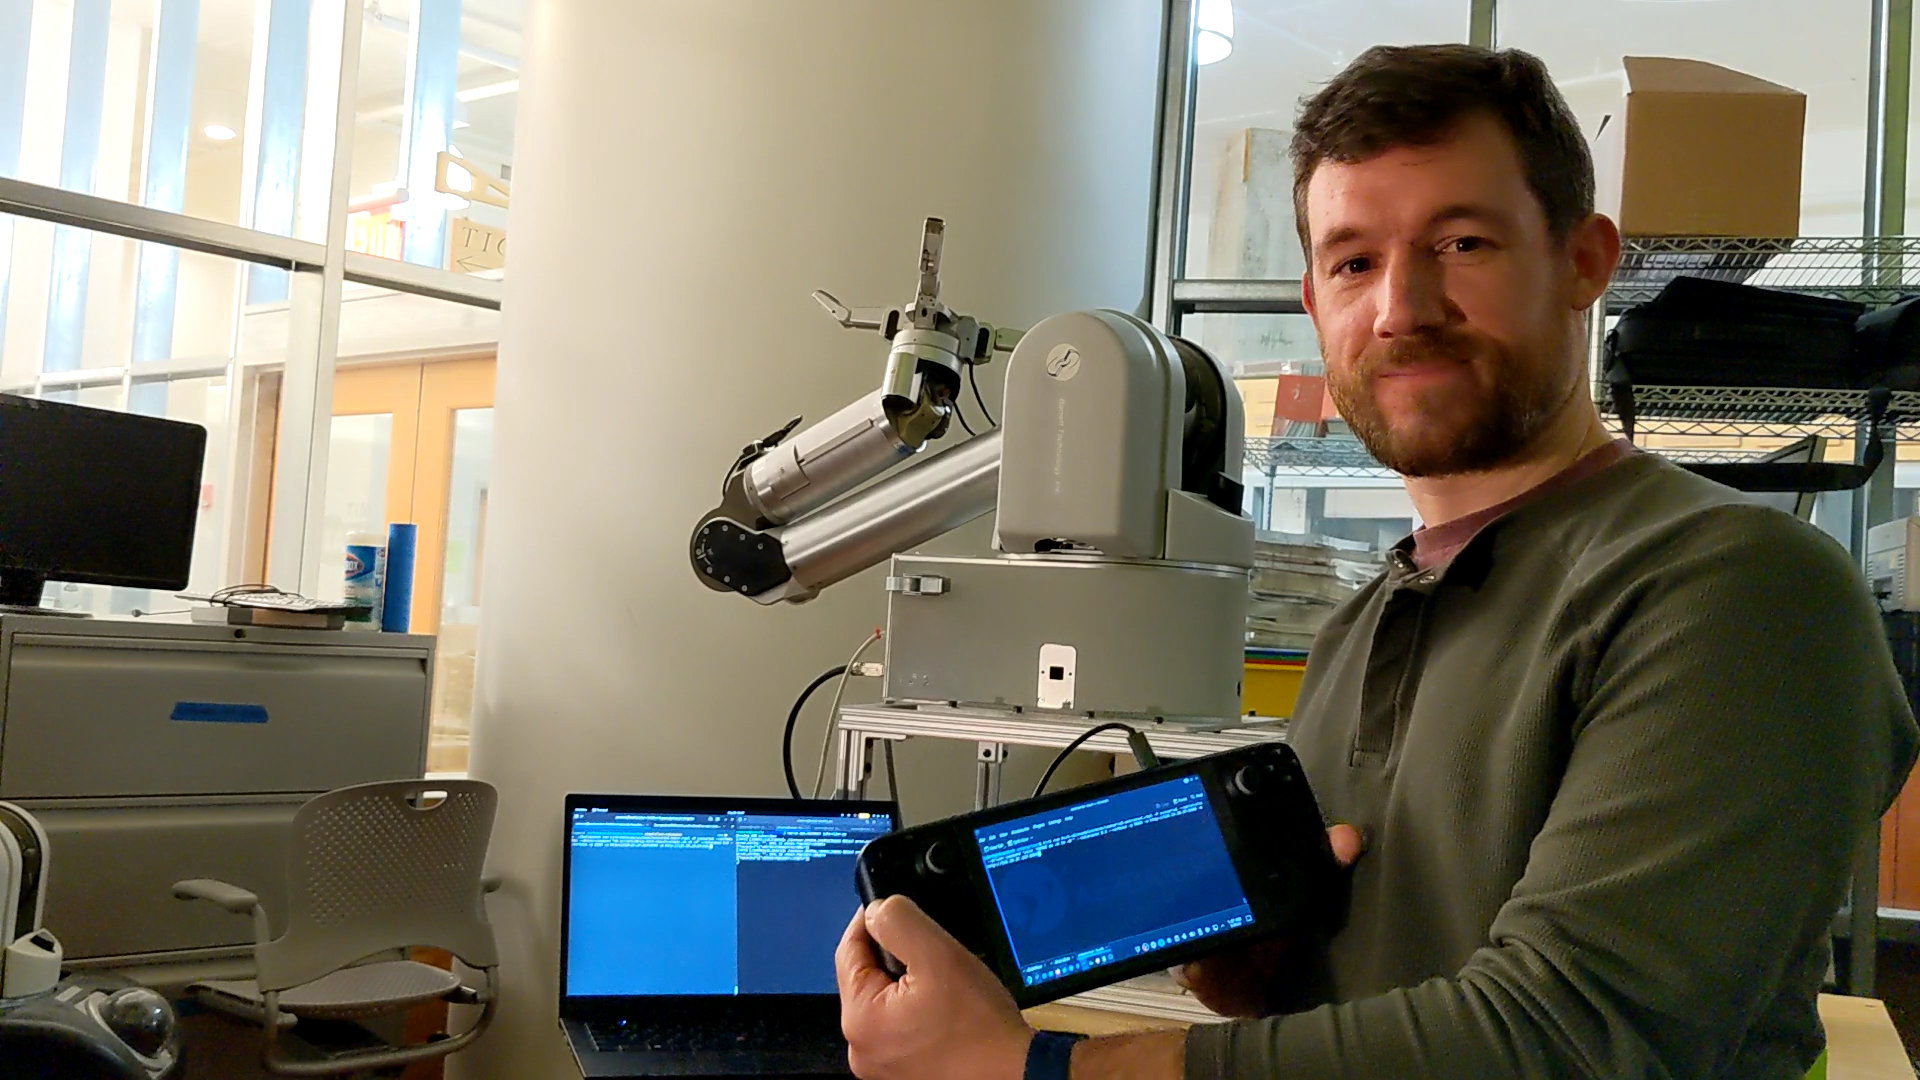
\includegraphics[width=\textwidth]{images/hw-demo-overview.png}
\caption{\label{fig:hw-demo-overview}The two Kirks and two agents of the hardware demonstration. The Kirk executive running on the laptop is controlling the Barrett WAM arm in the background. Cameron Pittman is the second agent (acting as the astronaut) and interacting with a Kirk executive running on the Steam Deck handheld PC. This image was taken in the MERS lab on 20 May 2023.}
\end{figure}

The architecture of the hardware demonstration is as shown in Figure \ref{fig:hw-demo-flowchart}. We ran
two Kirks on the same network. One Kirk was responsible for driving the Barrett WAM, while the other
acted as the decision making logic behind an interface on the astronaut's person (say a tablet,
heads-up-display, or portable computer of some kind).

\begin{figure}[htbp]
\centering
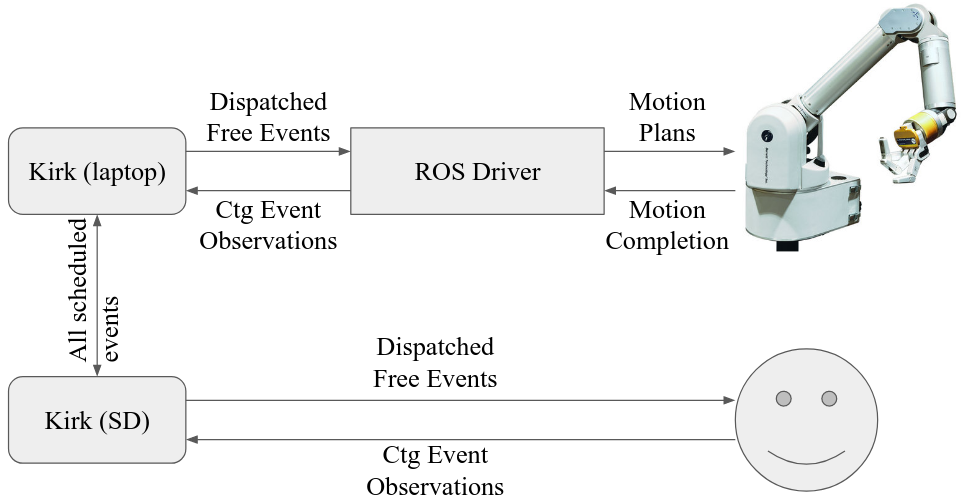
\includegraphics[width=0.8\textwidth]{images/hw-demo-flowchart.png}
\caption{\label{fig:hw-demo-flowchart}The information flow between the two agents and two Kirks in the hardware demonstration. ``SD'' is short for Steam Deck.}
\end{figure}

The laptop ran the Kirk that controls the WAM. It did so by dispatching requirement events to a
separate driver that could translate event names to pre-built trajectories for the WAM. The
trajectories were then published to the WAM's controller as ROS messages. As trajectories were
completed, ROS messages were received by the ROS driver layer, which then sent contingent event
observations back to Kirk.

\begin{figure}[htbp]
\centering
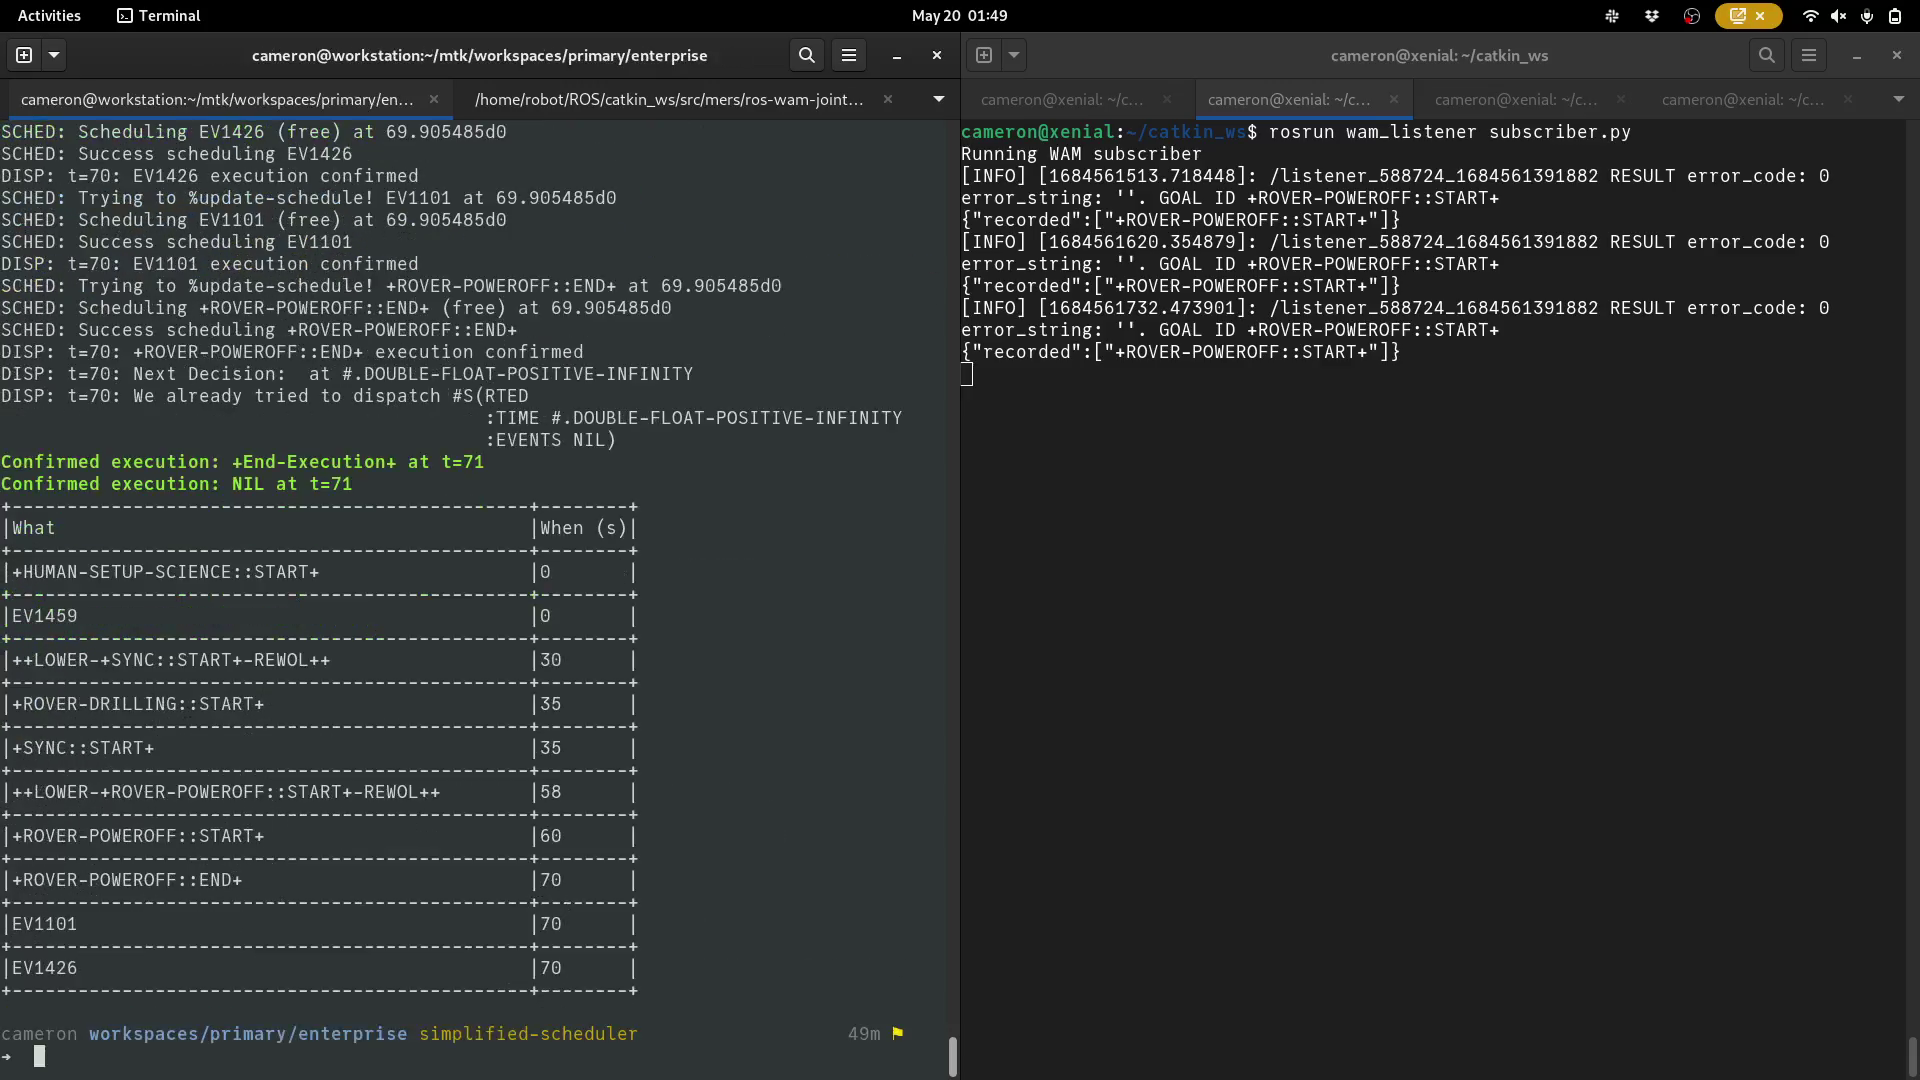
\includegraphics[width=\textwidth]{images/hw-demo-laptop-screen.png}
\caption{\label{fig:hw-demo-laptop-screen}The laptop screen at the end of the second hardware demo scenario. On the left is Kirk's output, on the right is the ROS translation layer. Kirk is showing the schedule that it executed, while we can see logs from messages sent between Kirk and the ROS layer on the right.}
\end{figure}

The Valve Steam Deck (SD), a handheld PC, ran the astronaut's Kirk. The Kirk command line tool
allows users to press a number to trigger the observation of a contingent event. We modified the
output of the video game controller buttons of the Steam Deck such that they would automatically
input the number corresponding to the observation of a contingent event. As the astronaut, Cameron
only needed to press one button (mapped to left on the d-pad) during the run to trigger the
observation.

\begin{figure}[htbp]
\centering
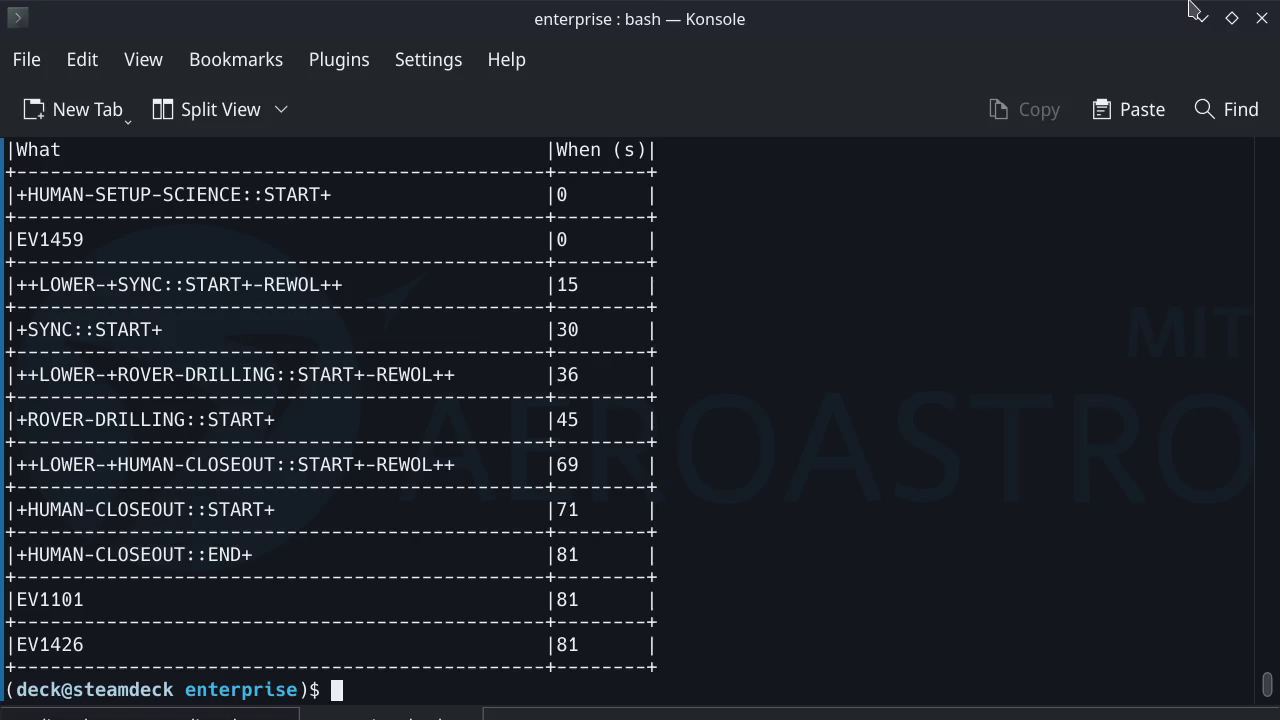
\includegraphics[width=\textwidth]{images/hw-demo-sd-screen.png}
\caption{\label{fig:hw-demo-sd-screen}The Steam Deck screen at the end of the second hardware demo scenario. On the left is Kirk's output, on the right is the ROS translation layer. Kirk is showing the schedule that it executed, while we can see logs from messages sent between Kirk and the ROS layer on the right.}
\end{figure}

The laptop and the Steam Deck were on the same local network. Note the cable dangling from the Steam
Deck in Figure \ref{fig:hw-demo-overview}, which is a USB-C to Ethernet adapter. The Steam Deck was
hardwired to the network for demonstration purposes. Communications occurred over HTTP. To simulate
uncertain communication, a sleep call with a time in the range of \(\gammabar(x_{c})\) was injected
into Kirk's function responsible for broadcasting event observations to peers, where
\(\gammabar(x_{c})\) was drawn from any contingent event \(x_{c} \in X_{c}\) of the receiving agent.

To start a run of the demonstration, we would start both Kirks simultaneously. Each Kirk had their
own RMPL control program, which we include in Listings \ref{code:astronaut-rmpl} and \ref{code:robot-rmpl}. Note
that the control programs are nearly identical. The control programs related to the high bandwidth
handoff, \texttt{human-downlink-science}, \texttt{sync}, and \texttt{robot-drilling}, differ only in observation delay
and whether the \texttt{sync} event is controllable. Adding observation delay reflects uncertain
communication between the agents.

The \texttt{sync} control programs were included as synchronization episodes between
\texttt{human-downlink-science} and \texttt{robot-drilling}. Note that the robot also has a \texttt{sync} episode, which
ensures that both agents agree on the naming of events.

\begin{listing}[htbp]
\begin{minted}[]{lisp}
(defpackage #:scenario1)

(in-package #:scenario1)

(define-control-program human-downlink-science ()
  (declare (primitive)
           (duration (simple :lower-bound 15 :upper-bound 30)
                     :contingent t)))

(define-control-program sync ()
  (declare (primitive)
           (duration (simple :lower-bound 5 :upper-bound 15
                             :min-observation-delay 0
                             :max-observation-delay 1)
                     :contingent t)))

(define-control-program robot-drilling ()
  (declare (primitive)
           (duration (simple :lower-bound 22 :upper-bound 26
                             :min-observation-delay 0
                             :max-observation-delay 2)
                     :contingent t)))

(define-control-program human-closeout ()
  (declare (primitive)
           (duration (simple :lower-bound 10 :upper-bound 30))))

(define-control-program main ()
  (with-temporal-constraint (simple-temporal :upper-bound 480)
    (sequence (:slack nil)
      (human-downlink-science)
      (sync)
      (robot-drilling)
      (human-closeout))))
\end{minted}
\caption{\label{code:astronaut-rmpl}The control program the astronaut uses while collecting and downlinking scientific data.}
\end{listing}

\begin{listing}[htbp]
\begin{minted}[]{lisp}
(defpackage #:scenario1)

(in-package #:scenario1)

(define-control-program human-downlink-science ()
  (declare (primitive)
           (duration (simple :lower-bound 15 :upper-bound 30
                             :min-observation-delay 5
                             :max-observation-delay 15)
                     :contingent t)))

(define-control-program sync ()
  (declare (primitive)
           (duration (simple :lower-bound 5 :upper-bound 15))))

(define-control-program robot-drilling ()
  (declare (primitive)
           (duration (simple :lower-bound 22 :upper-bound 26
                             :min-observation-delay 0
                             :max-observation-delay 1)
                     :contingent t)))

(define-control-program robot-poweroff ()
  (declare (primitive)
           (duration (simple :lower-bound 10 :upper-bound 30))))

(define-control-program main ()
  (with-temporal-constraint (simple-temporal :upper-bound 480)
    (sequence (:slack nil)
      (human-downlink-science)
      (sync)
      (robot-drilling)
      (robot-poweroff))))
\end{minted}
\caption{\label{code:robot-rmpl}The control program the robot uses to decide when to act with respect to learning the astronaut has finished collecting scientific data.}
\end{listing}

We can see the modeling power of variable observation delay in Listings \ref{code:astronaut-rmpl} and
\ref{code:robot-rmpl}. It is natural that the observation delay between agents may change due to the
evolution of resources during a mission. The variable-delay modeling framework allows us to model
uncertain delay for each temporal constraint independently. For instance, if we know that, say,
agents will be distant during a given constraint, then we may add uncertain delay accordingly. If
agents are collocated during other constraints, then we can safely decrease the observation delay
(absent other sources of delay).

According to the constraints and variable delay of the \texttt{human-downlink-science} control program from
the perspective of the robot, the transformed fixed-delay STNU the robot is executing will reflect
constraints of
\(\conedge{\texttt{human-downlink-science:start}}{\texttt{human-downlink-science:end}}{[30, 35]}\)
with \(\gamma(\texttt{human-downlink-science:end}) = 0\) after applying Lemma \ref{lemma:main-tightening}.

We performed two demonstrations. In the first, the astronaut would observe the end of the science
downlink, the end event of \texttt{human-downlink-science:end}, which would trigger a delayed observation
being passed to the robot. Once the robot received the command, it would begin its \texttt{robot-drilling}
activity. It passed observations of its scheduled events back to the astronaut.

\begin{figure}[htbp]
\centering
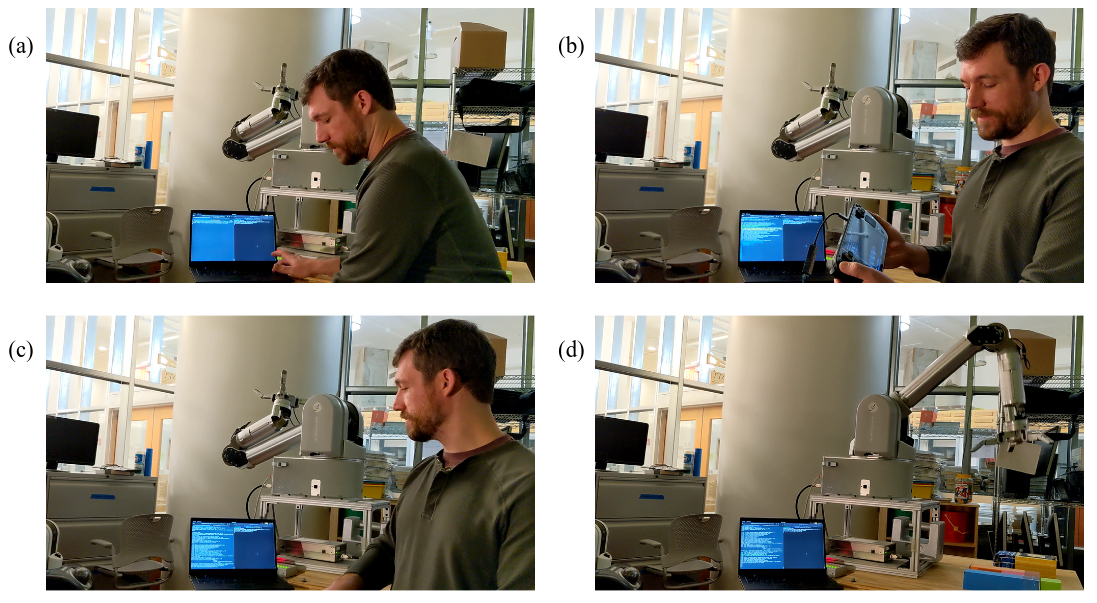
\includegraphics[width=\textwidth]{images/hw-demo-1-quad.png}
\caption{\label{fig:hw-demo-1-quad}The first demonstration in four parts. (a) \(t = 0\), when the two Kirks are started at the same time (unfortunately, the SD is below the image frame). (b) \(t = 16\), when the astronaut observed that the science experiment was setup. (c) \(t = 23\), when the robot received a delayed observation from the astronaut indicating they had completed science setup. (d) \(t > 23\), as the robot performed the drilling task.}
\end{figure}

The second demonstration focused on the behavior of the delay scheduler when communications are not
received in time. After starting both Kirks at the same time, we unplugged the astronaut's Kirk from
the network. While, in reality, a disconnection should be modeled as \(\gammabar^+(x_{c}) = \infty\),
we did it to emphasize the fact that the robot's Kirk would not receive an observation within the
fixed bounds it was expecting. The delay scheduler would then imagine \texttt{human-downlink-science:end}
and dispatch its drilling activity accordingly.

\begin{figure}[htbp]
\centering
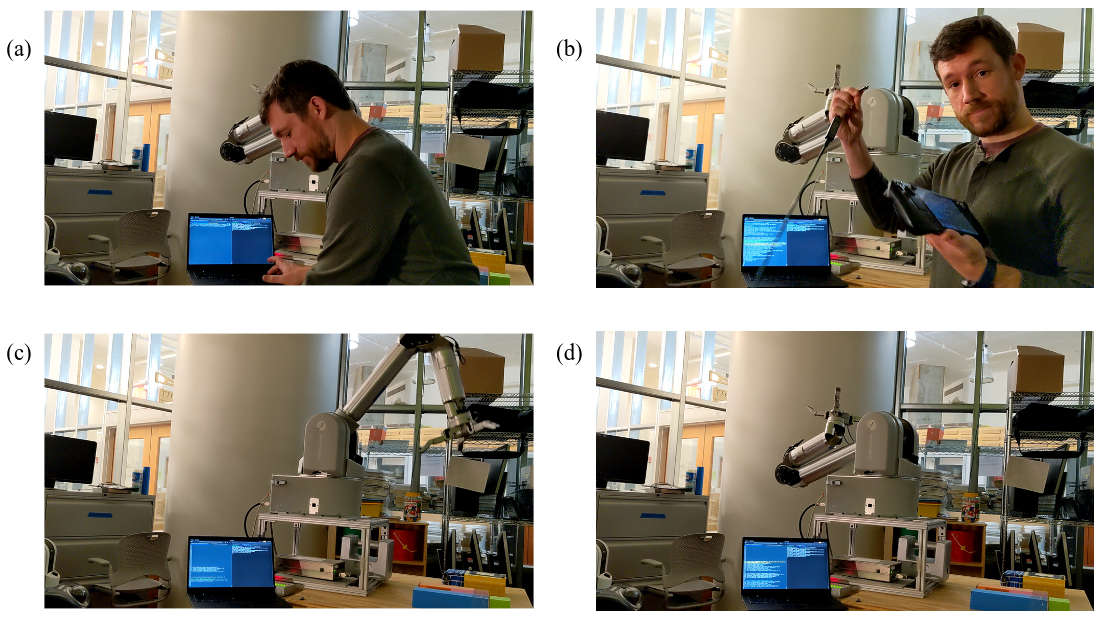
\includegraphics[width=\textwidth]{images/hw-demo-2-quad.png}
\caption{\label{fig:hw-demo-2-quad}The second demonstration in four parts. (a) \(t = 0\), when the two Kirks are started at the same time (unfortunately, the SD is below the image frame again). (b) \(t = 3\), when the SD is removed from the network. (c) \(t = 38\), after the robot imagined an observation from the astronaut and began the drilling task. (d) \(t = 60\), when Kirk has observed the end of the drilling task.}
\end{figure}

We present the schedules of the agents for both scenarios in Tables
\ref{table:hw-demo-1-astronaut}-\ref{table:hw-demo-2-robot}. The schedule has been cleaned and the event names
have been modified to better reflect the intent of the RMPL control programs. See Appendix
\ref{appendix:rmpl} for an explanation of how RMPL and the STNUs compiled from it are related. We also
removed anonymous (non-named) events that were added in the process of translating RMPL to
variable-delay STNU.

\begin{table}[htbp]
\caption{\label{table:hw-demo-1-astronaut}The complete history of the delay scheduler for the astronaut in the first hardware demo scenario.}
\centering
\begin{tabular}{lr}
\textbf{Event} & \textbf{Time (s)}\\\empty
\hline
Start Human Setup Science & 0\\\empty
Normalized Lower for End Human Setup Science & 15\\\empty
End Human Setup Science & 16\\\empty
Start Sync & 16\\\empty
Normalized Lower for Sync & 22\\\empty
End Sync & 23\\\empty
Start Robot Drilling & 23\\\empty
Normalized Lower for Robot Drilling & 47\\\empty
End Robot Drilling & 49\\\empty
Start Close Out & 49\\\empty
End Close Out & 59\\\empty
\end{tabular}
\end{table}

\begin{table}[htbp]
\caption{\label{table:hw-demo-1-robot}The complete history of the delay scheduler for the robot in the first hardware demo scenario.}
\centering
\begin{tabular}{lr}
\textbf{Event} & \textbf{Time (s)}\\\empty
\hline
Start Human Setup Science & 0\\\empty
Normalized Lower for Human Setup Science & 15\\\empty
End Human Setup Science & 22\\\empty
Start Sync & 22\\\empty
End Sync & 22\\\empty
Start Robot Drilling & 22\\\empty
Normalized Lower for Robot Drilling & 45\\\empty
End Robot Drilling & 46\\\empty
Start Robot Poweroff & 46\\\empty
End Robot Poweroff & 56\\\empty
\end{tabular}
\end{table}

We can see variable observation delay at work by comparing the assigned end times for
\texttt{human-setup-science} between the astronaut and robot in Tables \ref{table:hw-demo-1-astronaut} and
\ref{table:hw-demo-1-robot}. The human knows that science setup was completed at \(t = 16\), but the robot
received an observation of the same event after an apparently delay of six seconds.

Note that the robot was running an experimental \emph{optimistic} version of the delay scheduler in the
demonstration. The difference between the delay scheduler as described in Chapter
\ref{ch:delay-scheduling} and the optimistic version is that the optimistic version will attempt to avoid
buffering early contingent events by rewriting the delay STNU based on the early observation and
checking VDC. It will be discussed in more depth in Section \ref{sec:optimistic-rescheduling}.

\begin{table}[htbp]
\caption{\label{table:hw-demo-2-astronaut}The complete history of the delay scheduler for the astronaut in the second hardware demo scenario.}
\centering
\begin{tabular}{lr}
\textbf{Event} & \textbf{Time (s)}\\\empty
\hline
Start Human Setup Science & 0\\\empty
Normalized Lower for End Human Setup Science & 15\\\empty
End Human Setup Science & 30\\\empty
Start Sync & 30\\\empty
Normalized Lower for Sync & 36\\\empty
End Sync & 45\\\empty
Start Robot Drilling (imagined) & 45\\\empty
Normalized Lower for Robot Drilling & 69\\\empty
End Robot Drilling (imagined) & 71\\\empty
Start Close Out & 71\\\empty
End Close Out & 81\\\empty
\end{tabular}
\end{table}

\begin{table}[htbp]
\caption{\label{table:hw-demo-2-robot}The complete history of the delay scheduler for the robot in the second hardware demo scenario.}
\centering
\begin{tabular}{lr}
\textbf{Event} & \textbf{Time (s)}\\\empty
\hline
Start Human Setup Science & 0\\\empty
Normalized Lower for Human Setup Science & 30\\\empty
End Human Setup Science (imagined) & 35\\\empty
Start Sync & 35\\\empty
End Sync & 35\\\empty
Start Robot Drilling & 35\\\empty
Normalized Lower for Robot Drilling & 58\\\empty
End Robot Drilling & 60\\\empty
Start Robot Poweroff & 60\\\empty
End Robot Poweroff & 70\\\empty
\end{tabular}
\end{table}

Finally, we see in the second experiment that the robot was forced to imagine contingent events due
to communication delay. The robot was able to satisfy all constraints with its drilling episode
despite not receiving communication from the astronaut about the end of the astronaut setting up the
science experiment.

\chapter{Conclusion and Future Work}
\label{sec:orgaaa05e4}
\label{ch:discussion}

\section{Optimistic Rescheduling}
\label{sec:orgc5939ba}
\label{sec:optimistic-rescheduling}

We return to problem of potentially unnecessary wait time created by the buffering execution
strategy described in Lemma \ref{lemma:buffering-imagining}. First, we use an example to demonstrate how
buffering early contingent events results in a reduction of the execution space. Then we contribute
a technique for managing event observations that circumvents the loss of execution space.

Consider the following variable-delay controllable STNU, which we will refer to as
\(\mathit{Bufferable}\).

$$
\vdelayedge{A}{B}{[1, 7]}{[1, 3]}
\edge{}{C}{[5, 9]}
$$

Following the semantics of the delay scheduler, we would first transform \(\mathit{Bufferable}\) to
its fixed-delay equivalent, \(\mathit{Bufferable}'\) by applying Lemma \ref{lemma:main-tightening}.

$$
\fdelayedge{A'}{B'}{[4, 8]}{0}
\edge{}{C'}{[4, 6]}
$$

If we assume \(A\) is executed at \(t = 0\), the only question is when to schedule \(C\) (or its
fixed-delay equivalent, \(C'\)). According to the semantics of \(\mathit{Buffering}\), if \(B\) is
observed at \(t = 2\), we know that \(B\) was assigned at \(t = 1\). Thus, we only need to wait until \(t =
6\) to schedule \(C\). However, the delay scheduler would schedule according the constraints found in
\(\mathit{Buffering}'\), wherein \(\assign(B') = 2\) falls earlier than the lower bound of
\(\conedge{A'}{B'}{[4, 8]}\), triggering Lemma \ref{lemma:buffering-imagining}. As a result, we act as if
\(\assign(B') = 4\) and then wait for the lower bound of \(\edge{B'}{C'}{[4, 6]}\). The end result is
that \(C'\) is assigned to a later time of \(t = 8\).

From a human mission manager perspective, this wait appears to be a waste. Time is money. And in the
case of planetary exploration, time is safety. If a NASA flight controller were to ask why your
software is telling astronauts on Moon to just stand there doing nothing, responding that your
algorithm \emph{does not know} if it is safe to act, would be unacceptable. Therefore, we contribute a
generate-and-test approach that looks for opportunities to avoid buffering when contingent events
arrive before their expected windows in the fixed-delay STNU. The goal of this method is to dispatch
future events earlier if possible.

At its core, optimistic rescheduling consists of copying the original variable-delay STNU then
rewriting it to reflect the resolution of uncertainty so far. Key to rewriting the variable-delay
STNU is narrowing the constraint and observation delay to match what was observed. We then
re-perform controllability checks. If controllable, we have a new schedule that removes the need to
buffer this contingent event. If not controllable, we do nothing, buffer the contingent event as
planned, and continue dispatching against the original schedule.

We now step through the Event Observations with optimistic rescheduling algorithm (Algorithm
\ref{alg:optimistic-rescheduling}) in detail.

\begin{algorithm}
\SetAlgoLined
\SetKwComment{Comment}{//}{}
\SetKwFunction{Return}{return}
\SetKwInput{Input}{Input}
\SetKwInput{Output}{Output}
\SetKwInput{Algorithm}{\textsc{Event Observations with Optimistic Rescheduling}}
\SetKwInput{Initialize}{Initialization}
\SetKwIF{If}{ElseIf}{Else}{if}{then}{else if}{else}{endif}

\Indm
\Input{Original VDC STNU $S$; Equivalent fixed-delay function $\gamma$\; Partial history $\xi$; Executed events map $\mathit{Ex}(S, x)$; Observed contingent event $x$; Normalized lower bound $\hat x$; Current time $t$;}
\Output{Boolean whether $x$ was successfully scheduled, VDC STNU}

\Indp
\Algorithm{}
\Indp

$\mathit{successp}, \mathit{bufferedp} \gets \mathtt{updateSchedule(S, x, t)}$\;

\If{$\neg \mathit{bufferedp}$} {
    \Return $\mathit{successp}, S$\;
}

$S^{\ast} \gets \mathtt{rewriteSTNU(S, x, t)}$\;

\If{$S^{\ast}$ is not variable-delay controllable} {
    \Return $\mathit{successp}, S$\;
}

\For{$\mathit{a}$ in $\xi$ \Comment{$\mathit{a}$ is an assignment}} {
    \If{$\gamma(\mathit{a[event]}) \neq \infty$} {
        $\mathtt{updateSchedule(\mathit{S^{\ast}}, \mathit{a[event]}, \mathit{a[time]} + \gamma(\mathit{a[event]}))}$;
    }
}

\For{$\mathit{event}$ in $\mathit{Ex(S)}$} {
     $\mathit{Ex}(S^{\ast}, x) \gets \mathit{Ex}(S, x)$
}

$\mathtt{updateSchedule(\mathit{S^{\ast}}, \hat x, t)}$\;
$\mathtt{updateSchedule(\mathit{S^{\ast}, x, t)}$\;

\Return $\mathtt{true}, S^{\ast}$\;

\caption{An Algorithm for observing contingent events with optimistic rescheduling.}
\label{alg:optimistic-rescheduling}
\end{algorithm}

We cannot know if an event is buffered if we do not attempt to schedule it. Our first step is to
schedule an event like normal. If scheduling is possible without buffering, we simply return whether
scheduling was successful.

If the event was buffered, then we begin to optimistically reschedule. We do so by tightening the
bounds of the original VDC STNU, \(S_{\mathit{original}}\), based on the observation we received,
which is the responsibility of Algorithm \ref{alg:rewrite-stnu}, implementing Lemma \ref{lemma:narrow-bounds}.

If the rewritten STNU, \(S^{\ast}\), is found to be VDC, we prepare to schedule it. First we iterate
through all the assignments in the partial schedule and make the same assignments against the new
STNU. When assignments are made, we subtract out the fixed observation delay. In this loop, we add
the observation delay back, lest it be subtracted from the original observation twice.

If any contingent events with infinite delay were observed, they would have been marked executed but
not assigned. We iterate through the executed events of \(S\) and mark the same events executed in
\(S^{\ast}\).

The distance graph, partial schedule, and executed events of \(S^{\ast}\) now match that of \(S\) before
\(x_{c}\) was received. We are almost safe to record a new observation. Lastly, we must address the
executable event representing the normalized lower bound of \(x_{c}\), \(\hat x_{c}\). During
scheduling, we would have received an RTED consisting of \(\langle l + \gammabar^+(x_{c}), \hat x_{c}
\rangle\). Given that \(x_{c}\) arrived before \(l + \gammabar^+(x_{c})\), we never would have assigned
\(\hat x_{c}\), so we assign \(\assign(\hat x_{c}) = t\) now. We finally update the schedule with the
contingent event that arrived.

\begin{lemma}
\label{lemma:narrow-bounds}
If a contingent event, \(x_{c} \in X_{c}\), where \(u - l > \gammabar^+(x_{c}) - \gammabar^{-}(x_{c})\),
is observed at time \(t\) and when \(t < l + \gammabar^+(x_{c})\), we may replace \(x_{c}\) and
\(\gammabar(x_{c})\) with a constraint, \(x_{c}^{\ast}\), and variable-delay function,
\(\gammabar(x_{c}^{\ast})\), with narrower bounds as follows.

\begin{align*}
x_{c}^{\ast} &= [l^{\ast}, u^{\ast}] \\
x_{c}^{\ast} &= [\max(l, t - \gammabar^+(x_{c})), \min(u, t - \gammabar^{-}(x_{c}))] \\
\gammabar(x_{c}^{\ast}) &= [\max(\gammabar^{-}(x_{c}), t - u), \min(\gammabar^+(x_{c}), t - l)]
\end{align*}
\end{lemma}

\begin{proof}
Buffering is only possible if the conditions of Lemmas \ref{lemma:main-tightening} and
\ref{lemma:buffering-imagining} are triggered. By Lemma \ref{lemma:main-tightening}, we are guaranteed to be
able to narrow where in the range \([l, u]\) \(x_{c}\) was scheduled. By Lemma
\ref{lemma:buffering-imagining}, we know that rewritten bounds will lead to an assignment of \(x_{c}\) that
is no later than \(l + \gammabar^{+}(x_{c})\). Our tool for narrowing the bounds is Equation
\ref{eqn:fixed-recording}, which allows us to use the observation to reason over the assignment and
observation delay. Our strategy is to look at the extreme cases leading to an observation.

We start by reasoning over the earliest and latest assignments respectively. In order for \(x_{c}\) to
be assigned as early as possible, \(l^{\ast}\), we assume the delay has taken on its maximum value,
\(\gammabar^+(x_{c})\).

\begin{align}
\assign(x_{c}) &= \obs(x_{c}) - \gamma(x_{c}) \\
l^\ast &= t - \gammabar^+(x_c) \label{eqn:l-ast}
\end{align}

Likewise, to find the last possible assignment leading to an observation, we subtract the smallest
observation delay, \(\gammabar^{-}(x_{c})\).

\begin{align}
u^\ast = t - \gammabar^-(x_c) \label{eqn:u-ast}
\end{align}

Given that Nature will adhere to the constraints originally put forth in \(S\), the bounds of
\(x_{c}^{\ast}\) must remain within the bounds of \(x_{c}\). Hence, we guarantee the lower bound is at
least \(l\) while the upper bound is at most \(u\).

\begin{align*}
l^\ast &= \max(l, t - \gammabar^+(x_c)) \\
u^\ast &= \min(u, t - \gammabar^-(x_c))
\end{align*}

We use the same logic for narrowing the observation delay. If \(x_{c}\) was assigned as late as
possible, \(u\), then the observation delay would be minimized, \(\gammabar^-(x_{c}^{\ast})\). Likewise,
if \(x_{c}\) was assigned as early as possible, \(l\), the observation delay would be maximized,
\(\gammabar^+(x_{c}^{\ast})\). The narrowed lower and upper bounds of \(\gammabar(x_{c})^{\ast}\) are as
follows.

\begin{align*}
\gamma &= \obs(x_{c}) - \assign(x_{c}) \\
\gammabar^-(x_{c}^{\ast}) &= t - u \\
\gammabar^+(x_{c}^{\ast}) &= t - l \\
\end{align*}

As before, the bounds of \(\gammabar(x_{c}^{\ast})\) must stay within the original bounds of
\(\gammabar(x_{c})\), leaving us with the following narrowed observation delay.

\begin{align}
\gammabar^-(x_{c}^{\ast}) &= \max(\gammabar^{-}(x_{c}), t - u) \\
\gammabar^+(x_{c}^{\ast}) &= \min(\gammabar^+(x_{c}), t - l)
\end{align}
\end{proof}

We revisit the example from the beginning of this section to see Lemma \ref{lemma:narrow-bounds} in
action. As we saw before, any \(\obs(B)\) before \(t = 4\) will result in buffered assignments.

$$
\vdelayedge{A}{B}{[1, 7]}{[1, 3]}
\edge{}{C}{[5, 9]}
$$

Let \(t = 3\). We will step through the reasoning for narrowing the bounds of \(x_{c}\) accordingly.

\begin{align*}
x_{c}^{\ast} &\in [\max(l, t - \gammabar^+(x_{c})), \min(u, t - \gammabar^{-}(x_{c}))] \\
x_{c}^{\ast} &\in [\max(1, 3 - 3), \min(7, 3 - 1)] \\
x_{c}^{\ast} &\in [1, 2] \\
\\
\gammabar(x_{c}^{\ast}) &\in [\max(\gammabar^{-}(x_{c}), t - u), \min(\gammabar^+(x_{c}), t - l)] \\
\gammabar(x_{c}^{\ast}) &\in [\max(1, 3 - 7), \min(3, 3 - 1)] \\
\gammabar(x_{c}^{\ast}) &\in [1, 2]
\end{align*}

We find that \(\assign(x_{c})\) must have fallen somewhere in the range of \([1, 2]\), while
\(\gammabar(x_{c})\) was resolved somewhere in \([1, 2]\). Looking at the extremes, it is clear that
there are multiple combinations of the assignment and observation delay that could lead to an
observation at \(t = 3\). While the narrowed range allows for observations other than \(t = 3\), for
instance, if \(\assign(x_{c}) = 2\) and \(\obs(x_{c}) = 2\) yielding an observation at \(t = 4\), there
are no other ranges of assignments or observation delay outside of \(\assign(x_{c}) \in [1, 2]\) and
\(\gammabar(x_{c}) \in [1, 2]\) that would allow an observation at \(t = 3\).

\begin{algorithm}
\SetAlgoLined
\SetKwComment{Comment}{//}{}
\SetKwFunction{Return}{return}
\SetKwInput{Input}{Input}
\SetKwInput{Output}{Output}
\SetKwInput{Algorithm}{\textsc{Rewrite STNU}}
\SetKwInput{Initialize}{Initialization}
\SetKwIF{If}{ElseIf}{Else}{if}{then}{else if}{else}{endif}

\Indm
\Input{VDC STNU $S_{\mathit{original}}$; Variable-delay function $\gammabar$\; Observed contingent event $x$; Observation time $t$;}
\Output{VDC STNU}

\Initialize{$S_{\mathit{new}} \gets \mathtt{copy}(S_{\mathit{original}})$}

\Indp
\Algorithm{}
\Indp

\For{$\mathit{constraint}$ in $S_{\mathit{new}}$} {
    \If{$\mathit{constraint}$ ends in $x$} {
        $\mathit{constraint}[lower] \gets \max(\mathit{constraint}[lower], t - \gammabar^{+}(x))$\;
        $\mathit{constraint}[upper] \gets \min(\mathit{constraint}[upper], t - \gammabar^{-}(x))$\;
        $\gammabar^{-}(x) \gets \max(\gammabar^{-}(x), t - \mathit{constraint}[upper])$\;
        $\gammabar^{+}(x) \gets \max(\gammabar^{+}(x), t - \mathit{constraint}[lower])$\;
    }
}

\Return $S_{\mathit{new}}$\;

\caption{An Algorithm for rewriting an STNU given the resolution of uncertainty of a contingent link.}
\label{alg:rewrite-stnu}
\end{algorithm}

The complexity of Algorithm \ref{alg:optimistic-rescheduling} is dominated by the loop over
\texttt{updateSchedule}. Each call to \texttt{updateSchedule} is \(O(N^{3})\) in the number of events. In the worst
case scenario, every event up to the last contingent event has been scheduled, giving us a
complexity of \(O(N^{4})\). We discuss potential means for improving optimistic rescheduling in
Section \ref{sec:discussion-optimistic-rescheduling}.


\subsection{Possible Improvements}
\label{sec:org63f46d0}
\label{sec:discussion-optimistic-rescheduling}

What if we looked for conflicts? Could we possibly search for a time to dispatch early in the
buffered execution space?

Smarter rewriting STNU. Could we update the existing d-graph directly and check it for SRNCs? maybe?

\section{Coordination}
\label{sec:org2e81f59}
\label{sec:mastnus}

We were focused on addressing the multi-agent (MA) online scheduling problem. Before scheduling, we
must contend with planning, e.g. building variable-delay STNUs for each agent. We considered
extending the two existing planning approaches described below to model variable observation delay
between agents. We ultimately decided neither were fit for the motivating scenarios of this thesis.
Instead, we used a manual planning approach more akin to the ISS EVA planning process.

The first planning approach we considered was to model the system as a Multi-Agent STNU (MASTNU)
\citeprocitem{11}{[11]}. MASTNUs allow modelers to describe temporal constraints between multiple
agents, then check the overall dynamic controllability of the system. To check the controllability
of a MASTNU, the first step is to perform temporal decoupling with the goal of producing individual
dynamically controllable STNUs for each agent that can be dynamically scheduled per usual. While
superficially promising, there is a considerable drawback to this approach, namely that temporal
decoupling is sound but not complete, i.e. temporal decoupling may report failure even when the
MASTNU is dynamically controllable. This limits the utility of MASTNUs as a planning tool.

The other approach to this problem we are aware of is Stedl's Hierarchical Reformulation (HR)
algorithm \citeprocitem{45}{[45]}. HR begins with a MA temporal plan network (TPN), which is similar to a
MASTNU (though HR pre-dates MASTNUs). Stedl's key insight is to avoid inter-agent communication
altogether by reformulating constraints between groups of agents such that they are strongly
controllable. As such, no communication between agents is required. A centralized dispatcher is then
responsible for then handing events to agents. We also assume that there is no central authority,
making HR a poor fit for our problem domain.

Both MASTNUs and HR assume communications between agents are either instantaneous or impossible,
i.e. with an infinite delay. As we will see in Section \ref{sec:vdc}, our formalism for variable
observation delay allows a \emph{spectrum} of communication delay. While we felt it was possible to
shoehorn uncertain observation delay into MASTNUs or HR, we felt both were a poor choice because of
their pre-existing expectations with respect to communication. In combination with our focus on
online scheduling, we decided to forgo extending either formalism to account for observation delay.
Instead our planning process simply consists of manually writing variable-delay STNUs with
intra-agent and inter-agent temporal constraints by hand.

We believe it may be possible for MASTNUs or HR to be expanded to include variable observation
delay, though we leave that problem for future research.

We considered framing our approach to inter-agent communication as a distributed consensus problem
because we believed we needed a means for disparate agents to agree on the state of the world.
Existing distributed consensus algorithms like Paxos \citeprocitem{44}{[44]} or Raft \citeprocitem{43}{[43]}
would then be integrated into the communication layer of Kirk and take responsibility for ensuring
that agents agree on which events have been scheduled.

Ultimately the drawbacks of a distributed consensus approach outweighed the benefits. Chiefly, both
Paxos and Raft assume that communications are either instantaneous and freely available or that
agents have gone dark (i.e. can no longer communicate). This communication model is incongruous with
the explicitly modeled communications of the VDC formalism. Furthermore, the VDC formalism allows us
to model that agents never receive communications, negating the requirement for distributed
consensus.

\appendix

\chapter{Comparison of Variable-Delay STNUs to Partially Observable STNUs}
\label{sec:org3db369d}
\label{appendix:postnus}

The delay scheduler is flexible in that so long as it receives a variable-delay STNU, it is capable
of scheduling. Human modelers have flexibility in how they represent temporal constraints in that
there are many flavors of STNUs, each with their own advantages and disadvantages. Earlier, we
presented RMPL as a modeling language that is compiled to variable-delay STNUs. There are other
choices for modeling frameworks. Here, we present a comparison of variable-delay STNUs to POSTNUs
\citeprocitem{12}{[12]}, a flavor that is similar in many respects. This section presents a comparison
of variable-delay STNUs and POSTNUs, including transformations that allow some classes of POSTNUs to
be represented as variable-delay STNUs.

One of the strengths of the variable-delay controllability model is its ability to generalize the
concepts of strong and dynamic controllability. This technique was first seen in greater depth in
the context of POSTNUs. In an STNU, all contingent events are either
instantaneously observable under a dynamic controllability model or entirely unobservable under a
strong controllability model. In POSTNUs, contingent events can be marked observable and
unobservable. To say that a POSTNU is dynamically controllable equates to asserting that it is
possible to construct a schedule during execution that respects all constraints if the scheduler
only receives information about observable contingent events.

While, superficially, POSTNUs and delay STNUs appear to model distinct problems in temporal
reasoning, all delay STNUs can be accurately represented as POSTNUs. While the converse is not true,
there is a subset of POSTNUs that delay STNUs are able to model. It is advantageous to translate
POSTNUs to delay STNUs when possible because we are guaranteed to finish controllability checks for
delay STNUs in polynomial time, while evaluating the controllability of POSTNUs in general is harder
\citeprocitem{12}{[12]}. Furthermore, the sub-class of POSTNUs that can be checked efficiently and
accurately, those without chained contingent links \citeprocitem{46}{[46]}, are members of the
subset of POSTNUs that can be expressed directly as STNUs with fixed-delay, and likewise
variable-delay, functions , \citeprocitem{29}{[29, p. 59]}. The converse is also true - we may emulate
STNUs with variable-delay functions as POSTNUs without chained contingent links. Below, we elaborate
on translations from delay STNUs to POSTNUs, before describing how we can express POSTNUs without
chained contingent links as STNUs with fixed-delay functions. Note that this is not a comprehensive
list of transformations between delay STNUs and POSTNUs - our aim is to describe the minimum set of
transformations required to model POSTNUs without chained contingent links as delay STNUs. For the
following discussion, let \(S\) be a delay STNU and \(P\) be an equivalent POSTNU.

We present these transformations to demonstrate that the delay scheduler is capable of scheduling
POSTNUs without chained contingencies. So long as it receives a variable-delay STNU, the fact that
POSTNUs can be scheduled allows modelers additional flexibility in their means of representing the
problem domain.

We start with an \(S\) that consists of the links \(\conedge{A}{B}{}\) and \(\edge{B}{D}{}\) with delay
function \(\gammabar(B)\). See Figure \ref{fig:postnu} for an example translation between a fixed-delay STNU
and a POSTNU.

\begin{lemma}
\label{lemma:delay-stnu-to-postnu}
For contingent link \(\conedge{A}{B}{}\) in \(S\) with observation delay \(\gammabar(B) = [l, u]\), where
\(0 \leq l \leq u < \infty\), and outgoing requirement link \(\edge{B}{D}{}\), we may emulate
observation delay in \(P\) by copying \(\conedge{A}{B}{}\) and \(\edge{B}{D}{}\) to \(P\), enforcing that
\(B\) is unobservable, and adding a new observable contingent event, \(B'\) with \(\conedge{B}{B'}{[l,
u]}\).
\end{lemma}

\begin{proof}
In both \(S\) and \(P\), we do not observe \(B\) directly, yet we define an outgoing requirement link,
\(\edge{B}{D}{}\), that depends entirely on the resolution of \(B\). The only information available to
reason about the assignment of \(B\) comes in the form of an indirect observation, \(B'\) or
\(\gammabar(B)\), received after a delay in \(\mathbb{R}^{\geq 0}\). If \(P\) was not equivalent to \(S\),
we would be able to learn the assignment of \(B\) without waiting \(\gammabar(B)\) time units after its
true assignment. Thus, because we must wait \(B' - B \in [l, u]\) time units to learn the assignment
of \(B\), and \(\edge{B}{D}{}\) has equivalent constraints between \(S\) and \(P\), \(P\) must model the same
semantics as \(S\).
\end{proof}

\begin{lemma}
\label{lemma:postnu-observable}
For a contingent event \(B\) with variable-delay function \(\gammabar(B) = [0, 0]\) in \(S\), we may
emulate the same constraints with an observable contingent event, \(B\) in \(P\).
\end{lemma}

\begin{proof}
The variable-delay function enforces instantaneous observation. By the definition of observable
contingent events in the POSTNU model, we will observe \(B\) instantaneously.
\end{proof}

A POSTNU with a chained contingency is defined as follows. Consider a chain of contingent events,
\(\conedge{A}{B}{}\) and \(\conedge{B}{C}{}\). If \(B\) has one or more outgoing links to free or
contingent events other than \(C\), it is a chained contingency. Lemma \ref{lemma:delay-stnu-to-postnu}
results in a POSTNU without chained contingencies, hence variable-delay STNUs fall into the subclass
of POSTNUs that can be checked efficiently \citeprocitem{46}{[46]}.

In the other direction, to transform a POSTNU without chained contingencies into an STNU with
variable-delay functions, we need to address three cases of contingent constraints: (1) unobservable
contingent events not immediately followed by other contingent constraints, (2) unobservable
contingent events immediately followed by other contingent constraints, and (3) observable
contingent constraints.

\begin{lemma}
\label{lemma:postnu-unobservable}
For an unobservable event \(B\) in \(P\), with no outgoing contingent links, we can emulate it in \(S\)
with a contingent event \(B\) and upper bound of its variable-delay function set to \(\gammabar^+(B) =
\infty\).
\end{lemma}

\begin{proof}
We will not observe \(B\) nor will outgoing contingent links provide information about \(B\). As such we
define \(\gammabar^+(B) = \infty\) in \(S\).\footnote{Note: ,p. \citeprocitem{29}{[29, p. 60]} erroneously claims
that we should define \(\gamma(B) = 0\) for unobservable events.} From a controllability standpoint
for both \(S\) and \(P\), we know the \emph{a priori} bounds of \(B\) but will not learn its true assignment.
\end{proof}

\begin{lemma}
\label{lemma:combine-postnu-ctg}
For an unobservable contingent link \(\conedge{A}{B}{[m, n]}\) in \(P\), with a single outgoing link,
\(\conedge{B}{C}{[w, z]}\), we replace the two constraints from \(P\) in \(S\) with a concatenated
constraint, \(\conedge{A}{C}{[m+w, n+z]}\).
\end{lemma}

\begin{proof}
The only information we may receive is the observation of \(C\). Given there are no other outgoing
links from \(B\), folding \(B\) into the successive contingent constraint can not affect the semantics
of the network. The bounds of the new link, \(\conedge{A}{C}{[m + w, n + z]}\) is the result of
summing the intervals of \(\conedge{A}{B}{[m, n]}\) and \(\conedge{B}{C}{[w, z]}\): \([m, n] + [w, z] =
[m + w, n + z]\).
\end{proof}

Note that we did not specify whether \(C\) is observable in \(P\). After applying Lemma
\ref{lemma:combine-postnu-ctg}, we then apply either Lemma \ref{lemma:postnu-observable} or
\ref{lemma:postnu-unobservable} to \(C\).

\begin{lemma}
For an observable contingent event \(\conedge{A}{B}{[m, n]}\) in \(P\), with a single outgoing link to
an observable contingent event, \(C\), \(\conedge{B}{C}{[w, z]}\), we create three constraints in \(S\):
\(\conedge{A}{B}{[m, n]}\), \(\edge{B}{B'}{[0, 0]}\), and \(\conedge{B'}{C}{[w, z]}\) where \(\gammabar(B)
= [0, 0]\).
\end{lemma}

\begin{proof}
Given \(C\) is observable in \(P\), a simulated free event, \(B'\) in \(S\), can be scheduled simultaneously
with \(B\). Any contingent constraints following \(B\) now start at an executable event and are thus
valid constraints in \(S\). \(B\) is observable, so we need no observation delay according to Lemma
\ref{lemma:postnu-observable}.
\end{proof}

Thus, delay STNUs are sufficiently capable of expressing all POSTNUs that can efficiently be checked
for controllability using today's tractable POSTNU algorithms.

\begin{figure}[!htb]
\label{fig:postnu}
\caption{(a) An STNU with a contingent constraint that has a certain delay. (b) One possible way of rewriting the STNU as an equivalent POSTNU. This particular POSTNU exhibits a chained contingency, as $B$ is a contingent event that starts a contingent constraint and is connected to $B'$ via a contingent constraint.}
\centering
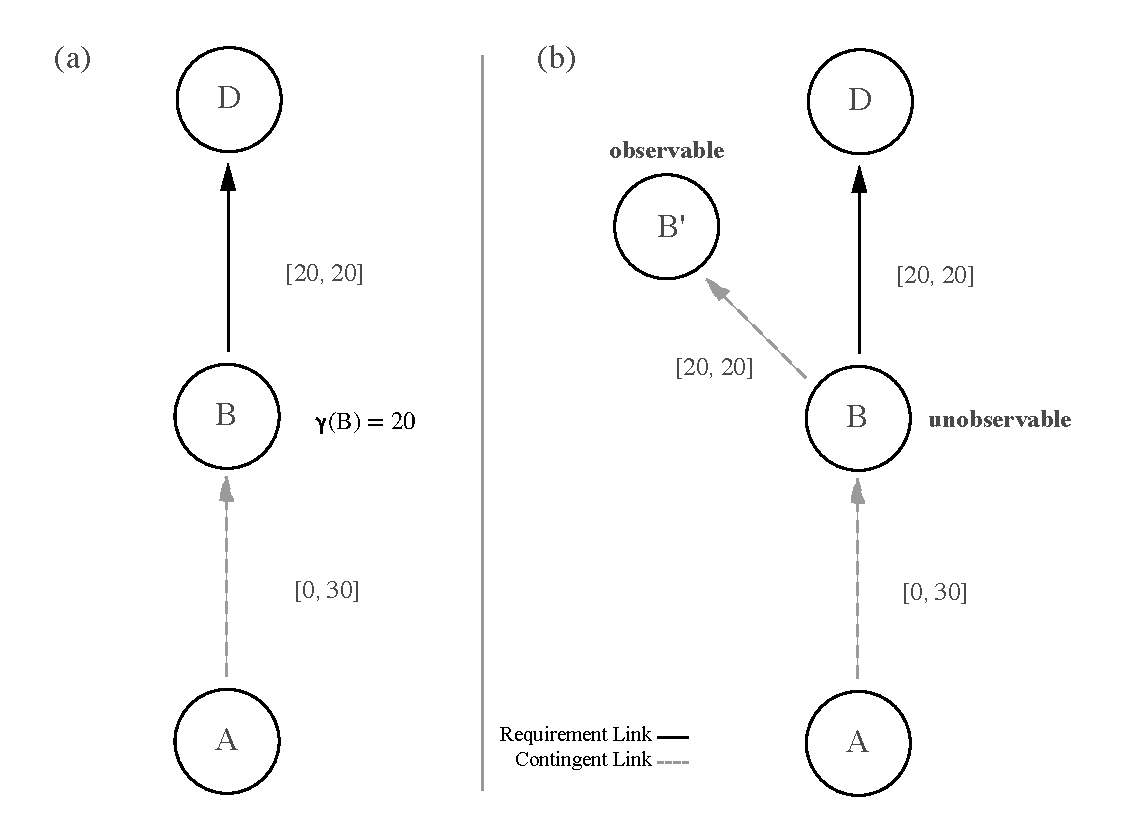
\includegraphics[width=0.75\textwidth]{POSTNU.pdf}
\end{figure}

It is not clear if controllability can be checked more efficiently across a greater subset of
POSTNUs beyond those without chained contingencies. However, it is worth highlighting that
variable-delay controllability can be leveraged to construct improved algorithms with respect to
scheduling and controllability of POSTNUs. The model for observation delay proposed by
variable-delay controllability can be expressed exactly as a POSTNU with a ``single-headed'' chained
contingency\footnote{To borrow the term ``single-headed'' from \citeprocitem{47}{[47]}.} as shown
in Figure \ref{fig:postnu}b; the main difference is that we represent the contingent link between \(B\) and
\(B'\) with our variable-delay function \(\gammabar(B)\). Hence, the algorithm we present for
variable-delay controllability can be used to both solve POSTNUs without chained contingencies, as
described above, as well as those POSTNUs with single-headed chained contingencies. Approaches
inspired by variable-delay controllability have been used to further expand POSTNU dynamic
controllability checking in more expressive chained instances \citeprocitem{47}{[47]}. We
hope that insights from variable-delay controllability will continue to expand the subset of POSTNUs
that can be controllability checked, and as such we advocate for continued development of the theory
of variable-delay controllability as a relevant framework for modelers.

\chapter{RMPL Control Programs and STNUs}
\label{sec:orgfe42e87}
\label{appendix:rmpl}

Key to the challenge of being a mission planner is to understand the constraints between events.
RMPL is an abstraction layer, meaning that it will interpret RMPL and produce a delay STNU
reflecting its own interpretation, which may not align with the mission planner's intention. We have
seen students in the lab be surprised by the temporal constraints generated by RMPL, and, through
the experiments involved in this thesis, have also found RMPL to be less-than-intuitive on occasion.
The chief cause of confusion is a disjoint between the fundamental unit of temporal reasoning, the
temporal event, and the fundamental unit of RMPL control programs, the episode, which consists of a
start and an end event. This is not a limitation of the semantics of RMPL, rather, it is a naming
issue.

To elaborate, temporal reasoning literature emphasizes events as meaningful timepoints. For
instance, we used numbered \texttt{Confirm:0:0} events to represent the end of an installation task in
Sections \ref{sec:scheduling-experimental} and \ref{sec:dkirk-simulation}, while the start of the task was an
\texttt{Install:0:0} event, e.g. \(\conedge{\texttt{Install:0:0}}{\texttt{Confirm:0:0}}{[l, u]}\). Depending
on the size of the generated STNU, the \texttt{Confirm:0:} event then had outgoing edges to events such as
\texttt{Start:0:1}, \texttt{Install:1:0}, or \texttt{ALL:END}. In RMPL, however, a representation of this constraint
between events with these names is impossible.

Consider the following control program.

\begin{minted}[]{lisp}
(define-control-program take-pictures ()
  (declare (primitive)
           (duration (simple :lower-bound 1 :upper-bound 5))))
\end{minted}

We have defined an episode named \texttt{take-pictures}. It represents a requirement constraint in the form
of \(\edge{\texttt{take-pictures:start}}{\texttt{take-pictures:end}}{[1, 5]}\). Note that the one
episode led to the creation of two events. We now add a second episode and show the two options RMPL
gives us for joining them in series.

\begin{minted}[]{lisp}
(define-control-program eat-snack ()
  (declare (primitive)
           (duration (simple :lower-bound 3 :upper-bound 7))))

;; Sequence option 1
(define-control-program with-slack ()
  (with-temporal-constraint (simple-temporal :lower-bound 6 :upper-bound 10)
    (sequence (:slack t)
              (take-pictures)
              (eat-snack))))

;; Sequence option 2
(define-control-program no-slack ()
  (with-temporal-constraint (simple-temporal :lower-bound 6 :upper-bound 10)
    (sequence (:slack nil)
              (take-pictures)
              (eat-snack))))
\end{minted}

We have two commonly used options for \texttt{:slack} in the sequence, \texttt{(:slack nil)} and \texttt{(:slack t)}. If
slack is applied, episodes are connected with \([0, \infty]\) constraints, effectively guaranteeing
episode ordering without enforcing that the latter episode must start immediately after the first.
Ignoring the overall constraint, the two control programs are connected like so.

$$
\edge{\texttt{take-pictures:start}}{\texttt{take-pictures:end}}{[3, 7]} \edge{}{\texttt{eat-snack:start}}{[0, \infty]} \edge{}{\texttt{eat-snack:end}}{[3, 7]}
$$

Without slack, the constraints are arranged as follows.

$$
\edge{\texttt{take-pictures:start}}{\texttt{take-pictures:end}}{[3, 7]} \edge{}{\texttt{eat-snack:start}}{[0, 0]} \edge{}{\texttt{eat-snack:end}}{[3, 7]}
$$

The RMPL compiler takes it a step further. A constraint of the form \(\edge{A}{B}{[0, 0]}\) enforces
simultaneous execution of \(A\) and \(B\), making one of the events redundant from a scheduling
perspective. In this example, RMPL removes \texttt{take-pictures:end}, leaving us with three events for the
two constraints.

$$
\edge{\texttt{take-pictures:start}}{\texttt{eat-snack:start}}{[3, 7]} \edge{}{\texttt{eat-snack:end}}{[3, 7]}
$$

From an execution perspective, \texttt{eat-snack:start} both signifies the end of taking pictures and the
beginning of snacking.

Going back to the installation example, we want the execution semantics of deciding when to start,
traversing to an installation location, performing the installation, waiting for the response, and
then moving to the next installation. As described in Section \ref{sec:scheduling-experimental}, the delay
STNU takes the form as follows, with \(\gammabar(\texttt{confirm:0:0}) = [0, 3]\).

$$
\conedge{\texttt{start:0:0}}{\texttt{traverse:0:0}}{[1, 15]} \edge{}{\texttt{install:0:0}}{[1, 14]} \conedge{}{\texttt{confirm:0:0}}{[1, 6]} \edge{}{\texttt{start:0:1}}{[2, 12]}
$$

In RMPL, we model each iteration of the procedure like so. (We use the \texttt{/0-0} numbering instead of
the \texttt{:0:0} scheme in RMPL because \texttt{:} causes errors related to lisp package exports.)

\begin{minted}[]{lisp}
(define-control-program traverse/0-0 ()
  (declare (primitive)
           (duration (simple :lower-bound 1 :upper-bound 15)
                     :contingent t)))

(define-control-program install/0-0 ()
  (declare (primitive)
           (duration (simple :lower-bound 1 :upper-bound 14))))

(define-control-program confirm/0-0 ()
  (declare (primitive)
           (duration (simple :lower-bound 1 :upper-bound 6
                             :min-observation-delay 0 :max-observation-delay 3)
                     :contingent t)))

(define-control-program start/0-1 ()
  (declare (primitive)
           (duration (simple :lower-bound 2 :upper-bound 12))))

(define-control-program main ()
  (with-temporal-constraint (simple-temporal :upper-bound 108)
    (sequence (:slack nil)
      (traverse/0-0)
      (install/0-0)
      (confirm/0-0)
      (start/0-1))))
\end{minted}

This results in a delay STNU of the form below (ignoring the overall upper-bound for simplicity's sake).

\begin{align*}
\conedge{\texttt{traverse/0-0:start}}{&\texttt{install/0-0:start}}{[1, 15]} \edge{}{\texttt{confirm/0-0:start}}{[1, 14]} \conedge{}{}{[1, 6]} \\
&\edge{\texttt{start/0-1:start}}{\texttt{start/0-1:end}}{[2, 12]}
\end{align*}

If we need to translate events between the two forms, we simply note that event names are shifted by
one place earlier in the delay STNU generated by RMPL.

%% This defines the bibliography file (main.bib) and the bibliography style.
%% If you want to create a bibliography file by hand, change the contents of
%% this file to a `thebibliography' environment.  For more information
%% see section 4.3 of the LaTeX manual.
\bibliography{extra-citations}
\begin{singlespace}
\begin{thebibliography}

\begin{hangparas}{1.5em}{1}
\hypertarget{citeproc_bib_item_1}{[1] D. A. Coan, “Exploration EVA System Concept of Operations,” National Aeronautics and Space Administration, Houston, TX, EVA-EXP-0042 Revision B, 2020.\\}

\hypertarget{citeproc_bib_item_2}{[2] J. W. McBarron, “Past, present, and future: The U.S. EVA Program,” \textit{Acta astronautica}, vol. 32, no. 1, pp. 5–14, 1994, doi: \href{https://doi.org/10.1016/0094-5765(94)90143-0}{10.1016/0094-5765(94)90143-0}.\\}

\hypertarget{citeproc_bib_item_3}{[3] C. P. Sonnett, “REPORT of the AD HOC WORKING GROUP ON APOLLO EXPERIMENTS AND TRAINING on the SCIENTIFIC ASPECTS OF THE APOLLO PROGRAM,” NASA, 1963.\\}

\hypertarget{citeproc_bib_item_4}{[4] J. M. Hurtado, K. Young, J. E. Bleacher, W. B. Garry, and J. W. Rice, “Field geologic observation and sample collection strategies for planetary surface exploration: Insights from the 2010 Desert RATS geologist crewmembers,” \textit{Acta astronautica}, vol. 90, no. 2, pp. 344–355, 2013, doi: \href{https://doi.org/10.1016/j.actaastro.2011.10.015}{10.1016/j.actaastro.2011.10.015}.\\}

\hypertarget{citeproc_bib_item_5}{[5] K. Young and T. Graff, “Planetary Science Context for EVA,” in \textit{NASA EVA Exploration Workshop}, 2020, p. 40.\\}

\hypertarget{citeproc_bib_item_6}{[6] A. Kanelakos, “Artemis EVA Flight Operations - Preparing for Lunar EVA Training \& Execution,” in \textit{NASA EVA Exploration Workshop}, 2020, p. 47.\\}

\hypertarget{citeproc_bib_item_7}{[7] M. J. Miller, “Decision Support System Development For Human Extravehicular Activity,” Georgia Institute of Technology, 2017.\\}

\hypertarget{citeproc_bib_item_8}{[8] M. Hiltz, C. Rice, K. Boyle, R. Allison, and M. D. Space, “CANADARM: 20 YEARS OF MISSION SUCCESS THROUGH ADAPTATION.”\\}

\hypertarget{citeproc_bib_item_9}{[9] R. Dechter, I. Meiri, and J. Pearl, “Temporal constraint networks,” \textit{Artificial intelligence}, vol. 49, no. 1-3, pp. 61–95, 1991, doi: \href{https://doi.org/10.1016/0004-3702(91)90006-6}{10.1016/0004-3702(91)90006-6}.\\}

\hypertarget{citeproc_bib_item_10}{[10] T. Vidal and H. Fargier, “Handling Contingency in Temporal Constraint Networks: From Consistency to Controllabilities,” \textit{Journal of experimental and theoretical artificial intelligence}, vol. 11, no. 1, pp. 23–45, 1999, doi: \href{https://doi.org/10.1080/095281399146607}{10.1080/095281399146607}.\\}

\hypertarget{citeproc_bib_item_11}{[11] G. Casanova, C. Pralet, C. Lesire, and T. Vidal, “Solving dynamic controllability problem of multi-agent plans with uncertainty using mixed integer linear programming,” \textit{Frontiers in artificial intelligence and applications}, vol. 285, pp. 930–938, 2016, doi: \href{https://doi.org/10.3233/978-1-61499-672-9-930}{10.3233/978-1-61499-672-9-930}.\\}

\hypertarget{citeproc_bib_item_12}{[12] M. D. Moffitt, “On the partial observability of temporal uncertainty,” \textit{Proceedings of the national conference on artificial intelligence}, vol. 2, pp. 1031–1037, 2007.\\}

\hypertarget{citeproc_bib_item_13}{[13] N. Bhargava, C. Muise, and B. C. Williams, “Variable-delay controllability,” in \textit{IJCAI International Joint Conference on Artificial Intelligence}, 2018, vol. 2018-July, pp. 4660–4666. doi: \href{https://doi.org/10.24963/ijcai.2018/648}{10.24963/ijcai.2018/648}.\\}

\hypertarget{citeproc_bib_item_14}{[14] L. Hunsberger, “A faster execution algorithm for dynamically controllable STNUs,” \textit{Proceedings of the 20th international symposium on temporal representation and reasoning}, pp. 26–33, 2013, doi: \href{https://doi.org/10.1109/TIME.2013.13}{10.1109/TIME.2013.13}.\\}

\hypertarget{citeproc_bib_item_15}{[15] L. Hunsberger, “Efficient execution of dynamically controllable simple temporal networks with uncertainty,” \textit{Acta informatica}, vol. 53, no. 2, pp. 89–147, 2016, doi: \href{https://doi.org/10.1007/s00236-015-0227-0}{10.1007/s00236-015-0227-0}.\\}

\hypertarget{citeproc_bib_item_16}{[16] M. Ingham, R. Ragno, A. Wehowsky, and B. Williams, “The Reactive Model-based Programming Language,” MIT Space Systems and Artificial Intelligence Laboratories, 2002.\\}

\hypertarget{citeproc_bib_item_17}{[17] Stanford Artificial Intelligence Laboratory et al., “Robotic operating system.” May 2018.\\}

\hypertarget{citeproc_bib_item_18}{[18] G. Daines, “Commercial lunar payload services.” NASA, Mar. 2019.\\}

\hypertarget{citeproc_bib_item_19}{[19] Consultative Committee for Space Data Systems, “CCSDS File Delivery Protocol (CFDP),” no. July, p. 151, 2020.\\}

\hypertarget{citeproc_bib_item_20}{[20] C. Campbell, “Advanced EMU Portable Life Support System (PLSS) and Shuttle/ISS EMU Schematics, a Comparison,” \textit{42nd international conference on environmental systems}, pp. 1–18, 2012, doi: \href{https://doi.org/10.2514/6.2012-3411}{10.2514/6.2012-3411}.\\}

\hypertarget{citeproc_bib_item_21}{[21] D. A. Coan, “Exploration EVA System Concept of Operations Summary for Artemis Phase 1 Lunar Surface Mission,” NASA, Houston, TX, 2020.\\}

\hypertarget{citeproc_bib_item_22}{[22] M. A. Seibert, D. S. Lim, M. J. Miller, D. Santiago-Materese, and M. T. Downs, “Developing Future Deep-Space Telecommunication Architectures: A Historical Look at the Benefits of Analog Research on the Development of Solar System Internetworking for Future Human Spaceflight,” \textit{Astrobiology}, vol. 19, no. 3, pp. 462–477, Mar. 2019, doi: \href{https://doi.org/10.1089/ast.2018.1915}{10.1089/ast.2018.1915}.\\}

\hypertarget{citeproc_bib_item_23}{[23] M. J. Miller and K. M. Feigh, \textit{Addressing the envisioned world problem: A case study in human spaceflight operations}, vol. 5. Cambridge University Press, 2019. doi: \href{https://doi.org/10.1017/dsj.2019.2}{10.1017/dsj.2019.2}.\\}

\hypertarget{citeproc_bib_item_24}{[24] M. J. Miller, K. M. McGuire, and K. M. Feigh, “Information flow model of human extravehicular activity operations,” \textit{Ieee aerospace conference proceedings}, vol. 2015-June, 2015, doi: \href{https://doi.org/10.1109/AERO.2015.7118942}{10.1109/AERO.2015.7118942}.\\}

\hypertarget{citeproc_bib_item_25}{[25] M. J. Miller, K. M. McGuire, and K. M. Feigh, “Decision Support System Requirements Definition for Human Extravehicular Activity Based on Cognitive Work Analysis,” \textit{Journal of cognitive engineering and decision making}, vol. 11, no. 2, pp. 136–165, 2017, doi: \href{https://doi.org/10.1177/1555343416672112}{10.1177/1555343416672112}.\\}

\hypertarget{citeproc_bib_item_26}{[26] A. Sehlke \textit{et al.}, “Requirements for Portable Instrument Suites during Human Scientific Exploration of Mars,” vol. 19, no. 3, pp. 401–425, 2019, doi: \href{https://doi.org/10.1089/ast.2018.1841}{10.1089/ast.2018.1841}.\\}

\hypertarget{citeproc_bib_item_27}{[27] P. H. Morris, N. Muscettola, and T. Vidal, “Dynamic Control Of Plans With Temporal Uncertainty,” 2001.\\}

\hypertarget{citeproc_bib_item_28}{[28] N. Bhargava, C. Muise, T. Vaquero, and B. Williams, “Delay Controllability : Multi-Agent Coordination under Communication Delay,” Massachusetts Institute of Technology, Cambridge, MA, 2018.\\}

\hypertarget{citeproc_bib_item_29}{[29] N. Bhargava, “Multi-Agent Coordination under Limited Communication,” Massachusetts Institute of Technology, 2020.\\}

\hypertarget{citeproc_bib_item_30}{[30] R. Bellman, “ON A ROUTING PROBLEM,” no. 1.\\}

\hypertarget{citeproc_bib_item_31}{[31] P. Morris, “A structural characterization of temporal dynamic controllability,” \textit{Lecture notes in computer science (including subseries lecture notes in artificial intelligence and lecture notes in bioinformatics)}, vol. 4204 LNCS, pp. 375–389, 2006, doi: \href{https://doi.org/10.1007/11889205_28}{10.1007/11889205\_28}.\\}

\hypertarget{citeproc_bib_item_32}{[32] P. Morris and N. Muscettola, “Temporal dynamic controllability revisited,” \textit{Proceedings of the national conference on artificial intelligence}, vol. 3, pp. 1193–1198, 2005.\\}

\hypertarget{citeproc_bib_item_33}{[33] N. Bhargava, C. Muise, T. Vaquero, and B. Williams, “Managing communication costs under temporal uncertainty,” in \textit{IJCAI International Joint Conference on Artificial Intelligence}, 2018, vol. 2018-July, pp. 84–90. doi: \href{https://doi.org/10.24963/ijcai.2018/12}{10.24963/ijcai.2018/12}.\\}

\hypertarget{citeproc_bib_item_34}{[34] L. Hunsberger, “Fixing the semantics for dynamic controllability and providing a more practical characterization of dynamic execution strategies,” \textit{Time 2009 - 16th international symposium on temporal representation and reasoning}, pp. 155–162, 2009, doi: \href{https://doi.org/10.1109/TIME.2009.25}{10.1109/TIME.2009.25}.\\}

\hypertarget{citeproc_bib_item_35}{[35] P. Virtanen \textit{et al.}, “SciPy 1.0: Fundamental algorithms for scientific computing in python,” \textit{Nature methods}, vol. 17, pp. 261–272, 2020, doi: \href{https://doi.org/10.1038/s41592-019-0686-2}{10.1038/s41592-019-0686-2}.\\}

\hypertarget{citeproc_bib_item_36}{[36] F. Pedregosa \textit{et al.}, “Scikit-learn: Machine learning in Python,” \textit{Journal of machine learning research}, vol. 12, pp. 2825–2830, 2011.\\}

\hypertarget{citeproc_bib_item_37}{[37] J. D. Hunter, “Matplotlib: A 2D graphics environment,” \textit{Computing in science \& engineering}, vol. 9, no. 3, pp. 90–95, 2007, doi: \href{https://doi.org/10.1109/MCSE.2007.55}{10.1109/MCSE.2007.55}.\\}

\hypertarget{citeproc_bib_item_38}{[38] B. C. Williams, M. D. Ingham, S. H. Chung, and P. H. Elliott, “Model-based programming of intelligent embedded systems and robotic space explorers,” \textit{Proceedings of the ieee}, vol. 91, no. 1, pp. 212–236, 2003, doi: \href{https://doi.org/10.1109/JPROC.2002.805828}{10.1109/JPROC.2002.805828}.\\}

\hypertarget{citeproc_bib_item_39}{[39] B. C. Williams and R. J. Ragno, “Conflict-directed A* and its role in model-based embedded systems,” \textit{Discrete applied mathematics}, vol. 155, no. 12, pp. 1562–1595, 2007, doi: \href{https://doi.org/10.1016/j.dam.2005.10.022}{10.1016/j.dam.2005.10.022}.\\}

\hypertarget{citeproc_bib_item_40}{[40] P. Kim, B. C. Williams, and M. Abramson, “Executing reactive, model-based programs through graph-based temporal planning,” \textit{Ijcai international joint conference on artificial intelligence}, pp. 487–493, 2001.\\}

\hypertarget{citeproc_bib_item_41}{[41] G. Kiczales, J. Des Rivières, and D. G. Bobrow, \textit{The art of the metaobject protocol}. Cambridge, Mass: MIT Press, 1991.\\}

\hypertarget{citeproc_bib_item_42}{[42] M. Fox and D. Long, “PDDL2.1: An extension to PDDL for expressing temporal planning domains,” \textit{Journal of artificial intelligence research}, vol. 20, pp. 61–124, 2003, doi: \href{https://doi.org/10.1613/jair.1129}{10.1613/jair.1129}.\\}

\hypertarget{citeproc_bib_item_43}{[43] D. Ongaro and J. Ousterhout, “In search of an understandable consensus algorithm,” \textit{Proceedings of the 2014 usenix annual technical conference, usenix atc 2014}, pp. 305–319, 2014.\\}

\hypertarget{citeproc_bib_item_44}{[44] L. Lamport \textit{et al.}, “The Part-Time Parliment,” \textit{Acm transactions on computer systems}, vol. 16, no. 2, pp. 373–386, 1998, doi: \href{https://doi.org/10.1145/568425.568433}{10.1145/568425.568433}.\\}

\hypertarget{citeproc_bib_item_45}{[45] J. L. Stedl, “Managing Temporal Uncertainty Under Limited Communication: A Formal Model of Tight and Loose Team Coordination,” Massachusetts Institute of Technology, 2004.\\}

\hypertarget{citeproc_bib_item_46}{[46] A. Bit-Monnot, M. Ghallab, and F. Ingrand, “Which contingent events to observe for the dynamic controllability of a plan,” \textit{Ijcai international joint conference on artificial intelligence}, vol. IJCAI-16, no. July, pp. 3038–3044, 2016.\\}

\hypertarget{citeproc_bib_item_47}{[47] P. H. Morris and A. Bit-monnot, “Dynamic Controllability with Single and Multiple Indirect Observations,” in \textit{ICAPS 2019 - Proceedings of the 29th International Conference on Automated Planning and Scheduling}, 2019, p. 9.\\}\bigskip
\end{hangparas}

\end{thebibliography}
\end{singlespace}
\end{document}
\end{document}